\documentclass[fleqn,10pt]{wlscirep}
\usepackage[utf8]{inputenc}
\usepackage[T1]{fontenc}
\usepackage{graphicx} % Required for inserting images
\usepackage{multirow}
\usepackage{helvet} % for the Helvetica font
\usepackage{xcolor}
\usepackage{algorithm}
\usepackage{algpseudocode}
\usepackage{amsmath}
\usepackage{amssymb}

%=================================================================
%  Revision Markup Commands (must remain defined in the preamble)
%=================================================================
\newcommand{\revtag}[2]{[\textbf{R#1-C#2}]}
\newcommand{\Rone}[1]{\textcolor{red}{#1}}
\newcommand{\Rtwo}[1]{\textcolor{blue}{#1}}
\newcommand{\Rthree}[1]{\textcolor{purple}{#1}}


\title{A Hierarchical Deep Learning Approach to Clinically Interpretable Cardiac MRI Diagnosis}

\author[1]{Vitalii Slobodzian}
\author[1,*]{Oleksandr Barmak}
\author[1]{Pavlo Radiuk}
\author[2]{Liliana Klymenko}
\author[3,4]{Iurii Krak}
\affil[1]{Khmelnytskyi National University, Department of Computer Science, Khmelnytskyi, 29016, Ukraine}
\affil[2]{Shupyk National Healthcare University of Ukraine, Department of Family Medicine and Outpatient Care, Kyiv, 04112, Ukraine}
\affil[3]{Taras Shevchenko National University of Kyiv, Department of Theoretical Cybernetics, Kyiv, 03680, Ukraine}
\affil[4]{V.M. Glushkov Institute of Cybernetics, Laboratory of Communicative Information Technologies, Kyiv, 03187, Ukraine}

\affil[*]{barmako@khmnu.edu.ua}

%\keywords{cardiac MRI, heart pathology, explainable deep learning, segmentation, classification, interpretation}

\begin{abstract}
\Rone{\revtag{1}{1} % Action 1: Abstract replacement
We present a hierarchical pipeline for cine cardiac MRI that (i) localizes and segments LV, RV, and myocardium with structure-specialized U-Nets, (ii) classifies five diagnostic categories (NOR, ARV, HCM, MINF, DCM) using a cascade calibrated on clinically meaningful thresholds, and (iii) returns study-level, clinician-facing indices (ventricular volumes, ejection fractions, wall-thickness maps on the AHA 17-segment model). On ACDC, segmentation attains mean Dice of 0.974 (LV, ED), 0.947 (RV, ED), and 0.920 (MYO, ES). The cascade reaches 97\% overall accuracy, outperforming strong multiclass baselines. We quantify uncertainty via bootstrap confidence intervals and assess calibration with reliability curves. A slice-position-aware refinement and explicit papillary-muscle policy improve robustness at apical/basal slices. Cross-dataset tests on M\&Ms corroborate external validity.
}
\end{abstract}

\begin{document}

\flushbottom
\maketitle
\thispagestyle{empty}

\section*{Introduction}

Over recent years, artificial intelligence (AI) methods in medical diagnostics have enabled the processing of complex medical images, detecting abnormalities, and suggesting preliminary diagnoses, thereby assisting physicians in making informed decisions \cite{Morales:2024,Srinivasan:2025}. Such technologies can significantly increase the efficiency of diagnostic processes by reducing dependence on the human factor and providing more standardized approaches to data analysis \cite{Ball:2016}.

Cardiovascular diseases (CVDs) are the leading cause of death worldwide, claiming approximately 17.9 million lives each year \cite{WHO:2022}. Given the considerable impact of CVDs on public health, reliable methods for detecting cardiac pathologies are crucial for reducing morbidity rates. Cardiac magnetic resonance imaging (MRI) is critical in diagnosing and treating heart and surrounding tissue diseases. MRI of the heart allows for accurate assessment of anatomy, ventricular function, myocardial viability, the presence of myocardial inflammation, or occlusions in blood vessels. It is a primary noninvasive examination method that offers high resolution and specificity compared to other imaging techniques, such as computed tomography (CT) and ultrasound \cite{Counseller:2023}. MRI is often called the gold standard due to its accuracy, reliability, and specificity \cite{Rose:1996}.

Nowadays, cardiac MRIs employ standardized protocols to generate images for assessing left ventricular and right ventricular structures and functions, as well as comprehensive tissue characterization \cite{Kramer:2020}. Despite these standardizations, the intricate cardiac anatomy, organ shape and size variability, and various image artifacts present significant challenges. Artifacts can result from patient movement, metal implants, or specific technical equipment settings. For example, motion artifacts, commonly caused by inconsistent heartbeats and breathing during scanning, necessitate specialized techniques to minimize their impact and enhance image quality \cite{Haskell:2023}. These complexities render MRI scan analysis highly labor-intensive and resource-demanding.

Beyond technical challenges, the accuracy and objectivity of MRI interpretation are significantly influenced by human factors and cognitive biases. Physicians may experience confirmation or recency biases, leading to potential misdiagnoses or inappropriate treatments. Unconscious biases, including those related to race or gender, can also affect the quality of medical care, resulting in unequal access to healthcare services and disparate treatment outcomes among different patient groups \cite{DeBenedectis:2022,Meidert:2023}. Additionally, variability in physicians’ interpretations of the same clinical data complicates standardization and impairs diagnostic accuracy.

The “black box” problem inherent in AI systems, particularly those based on deep learning (DL) models, exacerbates these challenges. While AI can effectively process input data and generate outputs, the decision-making processes remain nontransparent due to the complexity of thousands of interacting parameters \cite{Radiuk:2024a}. This omission undermines trust in AI systems, limits their applicability in critical fields like medicine, and heightens the risks associated with incorrect or unjustified conclusions.

To address the black box issue, existing approaches focus on enhancing AI transparency through interpretation and visualization methods \cite{Shick:2024}. Techniques such as heatmaps to highlight significant image regions and visualization of feature importance enable a deeper understanding of how AI systems make decisions. These tools facilitate the validation of AI results and bolster user trust, which is crucial in high-stakes environments.

Automating diagnosis and treatment prescription using AI is theoretically feasible by accounting for all physiological indicators and individual patient features (e.g., body structure, allergies, drug responses). However, the practical implementation faces substantial challenges, including the immense scale, time, and financial costs required to organize and label such extensive datasets \cite{Radiuk:2021}. Moreover, specific subjective indicators, such as patient-reported well-being or pain thresholds, necessitate physician evaluation during consultations, as AI cannot easily quantify them. Consequently, patients with identical diagnoses and physiological indicators may receive different treatments based on individual physician assessments, which are sometimes justified.

Modern medical and computer science strives to minimize subjectivity in treatment. Integrating objective data and AI algorithms reduces the likelihood of biases, promoting a more standardized approach. Conversely, physicians’ subjective assessments allow for the consideration of unique aspects of patients that are difficult to formalize. Balancing objective AI-driven indicators with subjective clinical judgments can optimize diagnostic and treatment processes, ensuring both accuracy and individualized patient care.

Hence, it is necessary to balance objective indicators and subjective factors when making medical decisions. Objective data and AI algorithms can reduce the likelihood of biases by providing a more standardized approach. In contrast, a physician’s subjective assessment allows for considering unique aspects of patient well-being that are difficult to formalize. This balance may help optimize the diagnostic and treatment process, making it both accurate and individualized.

The main contributions of this paper are as follows:
\Rone{\revtag{1}{1} % Action 2: Contribution statement replacement
\begin{itemize}
    \item \textbf{Hierarchical segmentation with structure specialization.} We decompose localization and contouring into six models (three ROI localizers; three structure-specific contourers) and show consistent gains—particularly for RV and ES-phase myocardium—over single-stage baselines\cite{Ronneberger:2015,Hu:2023,daSilva:2024}.
    \item \textbf{Clinically calibrated cascade classification.} A four-step cascade reduces DCM/MINF confusion observed in prior work\cite{Isensee:2018,Khened:2019,Zheng:2019}, reports calibrated probabilities, and selects operating points aligned with clinical thresholds.
    \item \textbf{Interpretation aligned with practice.} We derive LV/RV volumes, EF, volume–mass ratios, and 17-segment wall-thickness maps consistent with imaging guidelines\cite{Szabo:2022,Watanabe:2022}, providing study-level summaries amenable to clinician review.
\end{itemize}
}

The paper is structured as follows: Section 2 reviews contemporary approaches to segmenting, classifying, and interpreting cardiac MRI data using DL. Section 3 describes the three proposed methods: A multi-stage segmentation technique integrating U-Net and ResNet architectures, a cascade classification procedure tailored for DCM, HCM, MINF, ARV, and NOR, and an interpretation method that highlights clinical features such as myocardial thickness and ejection fraction. Section 4 presents the results of the proposed methods, comparing them to state-of-the-art techniques. Section 5 draws final conclusions, addresses limitations, and outlines possible future research directions.

\section*{State of the Arts}

Below is an analysis of related works concerning (i) methods for segmenting cardiac MRIs, (ii) methods for classifying pathologies in MRI scans, and (iii) methods for interpreting the decisions produced by DL models.

\subsection*{Segmentation of Cardiac MRIs}

Traditional segmentation techniques, including edge detection-based segmentation \cite{Zhao:2005}, threshold-based segmentation \cite{Xu:2010}, and region-based image segmentation \cite{Cigla:2008}, are valued for their low computational complexity and high processing speed. However, these methods fall short in accuracy and quality compared to contemporary DL-based approaches \cite{Liu:2021}.

DL methods, particularly convolutional neural networks (CNNs), have advanced medical image segmentation by identifying complex patterns within data \cite{Berezsky:2024}. Architectures like U-Net \cite{Ronneberger:2015} and SegNet \cite{Badrinarayanan:2017} have demonstrated superior accuracy even with limited datasets. These models excel because they can learn hierarchical features and adapt through retraining with new data, improving over time. Nonetheless, their advantages come with significant drawbacks, including high computational resource requirements and the necessity for extensive labeled training data \cite{Ankenbrand:2021}. Additionally, the “black box” nature of DL models raises trust issues, prompting interest in “human-in-the-loop” \cite{Radiuk:2022} and “human-centric” \cite{Singh:2025} approaches to enhance transparency and reliability.

Hybrid segmentation techniques that integrate classical and DL approaches are gaining traction. For instance, combining CNN-based preprocessing with active contour models leverages the strengths of both methods, achieving precise boundary detection. Similarly, ensemble learning methods incorporating multiple DL models can enhance segmentation accuracy by addressing different aspects of the image-processing task. \Rone{\revtag{1}{8}These hierarchical or two-stage pipelines, some incorporating attention mechanisms, have shown promise in refining coarse initial segmentations \cite{Wang:2023b,Patil:2023}.} These hybrid strategies, while effective, demand more significant computational resources and complex model tuning. Specialized models tailored to specific cardiac regions have shown improved accuracy by focusing on unique anatomical features \cite{Wehbe:2023}.

Multimodal approaches that utilize multiple imaging modalities, such as combining CT and MRI data, aim to improve segmentation accuracy by integrating complementary information. However, these methods face significant challenges in dataset creation and integration, as aligning and harmonizing data from different sources is complex \cite{Pandey:2023,Azam:2022}. For example, Hu et al. \cite{Hu:2023} developed a deeply supervised network combined with a 3D Active Shape Model to reduce manual initialization efforts, achieving high accuracy but limited by substantial computational demands and lack of validation across varied imaging protocols. Similarly, da Silva et al. \cite{daSilva:2024} designed a cardiac segmentation technique for short-axis MRI that employs six fully CNNs. Their framework comprises one CNN dedicated to the region of interest (ROI) extraction, three CNNs for the initial segmentation phase, and two additional CNNs for the reconstruction stage. Despite this comprehensive approach, their methodology exhibited reduced performance on end-systolic (ES) slices compared to end-diastolic (ED) slices in most cases.

Other advanced models have also demonstrated strong performance on the ACDC dataset. For instance, Hasan and Linte \cite{Hasan:2020} introduced CondenseUNet, a memory-efficient architecture that achieved a Dice score of 0.901 for the myocardium. Zhang et al. \cite{Zhang:2022} proposed a nested capsule dense network (NCDNet), which reported a Dice coefficient of 0.903 for the myocardium in the end-diastolic phase and 0.918 in the end-systolic phase. These studies highlight the competitive landscape and underscore the need for methods that not only achieve high accuracy but also offer improvements in specific challenging areas, such as right ventricle delineation or end-systolic phase segmentation, which our work aims to address.

Self-supervised and semi-supervised learning methods have emerged as promising solutions to the scarcity of labeled medical data. Contrastive learning techniques \cite{Tian:2020,Chen:2020} have shown success by learning representations by distinguishing similar and dissimilar data samples. Recent studies \cite{Liu:2024,Felfeliyan:2023} have developed efficient self-supervised learning frameworks specifically for medical image segmentation, enabling models to learn robust features without extensive labeled datasets. These approaches significantly reduce the reliance on manual annotations, making them highly valuable for medical imaging applications where labeled data is limited.

Recent research has explored the integration of segmentation and classification tasks to streamline the diagnostic workflow. For instance, Zheng et al. \cite{Zheng:2019} employed semi-supervised learning for explainable DL to classify MRI scans yet encountered challenges with motion artifacts, highlighting the need for robust models to handle real-world imaging variances. Ammar et al. \cite{Ammar:2021} developed a combined segmentation-classification pipeline for diagnosing heart diseases, achieving enhanced accuracy but at the cost of increased training complexity. Bourfiss et al. \cite{Bourfiss:2023} introduced a corrective framework to address segmentation errors, which required manual intervention and increased workflow complexity.

Overall, while self-supervised methods offer significant advancements in medical image segmentation, they are computationally expensive and require numerous training iterations. Training such models typically necessitates robust computing infrastructure, making them less accessible for widespread clinical use.

\subsection*{Classification of Cardiac MRIs}

Traditional machine learning techniques, including support vector machines (SVM), decision trees, and ensemble methods like random forests, have been employed for medical image classification using handcrafted features such as textures and shapes. While these methods are suitable for more straightforward tasks, they are generally outperformed by DL models, especially when handling large and complex datasets \cite{Mofrad:2022}.

CNN architectures, notably ResNet \cite{He:2016} and DenseNet \cite{Huang:2017}, play a crucial role in medical image classification by automatically extracting intricate features from input data. DenseNet, in particular, has proven highly effective in tumor image classification by processing small patches from extensive digital pathological images \cite{Mofrad:2022}. These architectures facilitate the creation of highly accurate models capable of distinguishing subtle pathological differences.

Methodologies have been developed to enhance classification accuracy by integrating segmentation outputs with classification algorithms. For example, one approach \cite{Mofrad:2022} uses segmentation masks to extract time-series data on myocardial segment radius and thickness, constructing motion maps that inform a logistic regression model to classify five cardiac pathologies: DCM, HCM, MINF, ARV, and patients without cardiac disease (NOR). This method achieves high accuracy (95\% training, 94\% testing) while maintaining explainability and simplicity, crucial for clinical adoption.

Another study \cite{Isensee:2018} focuses on disease classification using cine-MRI data through a combined segmentation and classification model. Utilizing a U-Net for segmentation, the model extracts both static and dynamic features from segmented regions, including ventricular volume and myocardial thickness. These handcrafted features are then used to train an ensemble of multilayer perceptrons (MLPs) and a random forest classifier, achieving segmentation Dice coefficients of 0.945 (LV), 0.911 (myocardium), and 0.923 (RV), along with classification accuracies of 94\% (training) and 92\% (testing). However, this model struggles to differentiate between similar pathologies like DCM and MINF.

The classification approach in \cite{Khened:2019} integrates DL and ensemble classifiers for automated heart disease diagnosis from cine-MRI. Using DenseNet-based CNNs for segmentation, the method extracts clinically relevant features such as ventricular volumes and myocardial mass. An ensemble of classifiers (SVMs, MLPs, etc.) then classifies five categories (ARV, HCM, MINF, DCM, NOR), achieving high Dice coefficients (0.96 LV, 0.95 RV, 0.89 myocardium) and a classification accuracy of 100\%. However, the ensemble’s complexity and potential overfitting, particularly with smaller datasets, limit its practicality and ability to distinguish between similar pathologies without expert intervention.

\subsection*{Interpretation of DL Models}

A significant challenge in adopting AI in clinical settings is the interpretability of DL models. Overcoming the “black box” nature of these models is essential for building trust among clinicians. Current studies emphasize the use of heatmaps and saliency maps to visualize important image regions, thereby enhancing physician confidence and improving diagnostic accuracy for MRI and other medical scans \cite{Watanabe:2022}.

Research \cite{Ali:2024} highlights the expanding role of AI in cardiovascular diagnostics, noting improvements in accuracy and speed of image analysis, reduction of human errors, and minimized radiation exposure. These advancements underscore the potential of AI to rival expert clinicians while emphasizing the need for broader exploration across diverse cardiology applications. Guidelines outlined in \cite{Szabo:2022,Salih:2023} focus on evaluating trust in AI systems for medical imaging, emphasizing strategies to mitigate ethical and clinical risks. Ensuring alignment with clinical practices is vital for AI’s safe and effective deployment in diagnosing cardiac diseases.

The deep Taylor-CAV (D-TCAV) method discussed in \cite{Janik:2021} offers concept-based explanations for AI model decisions in cardiac image segmentation. By identifying key image regions that influence outcomes, such as uneven walls or chamber size differences, D-TCAV provides objective data that supports diagnostic analysis. This approach enhances transparency and reliability, reducing the risk of biased or arbitrary model decisions and fostering trust in AI-driven cardiology tools. It can be clearly observed that contemporary research underscores the importance of developing interpretable AI models to facilitate their integration into cardiology. Visualization and explanation tools are crucial for making AI outputs understandable to clinicians, thereby increasing the reliability and clinical accessibility of AI technologies for patient diagnosis and treatment.

In summary, related works demonstrate significant advancements in cardiac MRI segmentation and classification through DL models, while also addressing the need for interpretability and trust in AI systems. These developments highlight the potential of AI to enhance diagnostic accuracy and efficiency in cardiology, provided that challenges related to model transparency and ethical considerations are effectively managed.

\subsection*{Aim of the Study and Research Objectives}

From the above analysis of related works, the main goal of this research is to improve the quality of cardiac MRI scan segmentation and classification and to enable the interpretation of DL-based decisions. This goal is pursued through the following steps:

\begin{enumerate}
    \item Develop a multi-stage segmentation method for dividing the heart region in MRI scans into the RV, LV and myocardium. This method combines U-Net and ResNet models for localizing and segmenting cardiac structures, followed by Gaussian smoothing for contour refinement and artifact reduction.
    \item Develop a cascade classification method for pathologies—DCM, HCM, MINF, and ARV—in MRIs, to more accurately categorize heart pathologies using segmented MRI data.
    \item Develop a method for interpreting DL decisions based on clinical features commonly used in medical practice.
\end{enumerate}

\section*{Methods}

\Rthree{\revtag{3}{3}\subsection*{Datasets, Splits, and Preprocessing}}
\Rthree{\revtag{3}{9} % Action 3 & 9
We used the ACDC dataset\cite{Bernard:2018} with the official train/test partition (100/50 patients). For external validation, we used the M\&Ms dataset\cite{Campello:2021}. \emph{All} data splits for training, validation, and testing were performed at the patient level to prevent data leakage. For the classification task, per-patient image stacks (ED/ES) were augmented to create a uniform number of slices per patient; this augmentation was applied only within the training folds. No slice from a patient in the test or validation set ever appeared in the training set. 
}
\Rone{\revtag{1}{4} % Action 4
Region of interest (ROI) crops at test time are generated exclusively by the learned localizer models ($M_1$–$M_3$), ensuring no ground-truth information is used during inference. The Gaussian blur parameter, $\sigma$, used for post-processing, is not tuned per image. Instead, it is selected via a grid search on the validation set of the training data and then fixed for all test set inferences to prevent information leakage and ensure reproducibility. We additionally report an ablation study using ground-truth versus predicted ROIs to quantify the robustness of the localization stage.
}

It should be noted that this study focuses on detecting the following cardiac pathologies via MRI scans: DCM, HCM, MINF, and ARV. These particular pathologies were chosen due to their high prevalence and clinical significance. They are among the most common heart diseases \cite{Wang:2023,McKenna:2017}, characterized by a range of morphological and functional changes that MRI can detect. Publicly available, high-quality dataset titled Automated Cardiac Diagnosis Challenge (ACDC) \cite{Bernard:2018} includes annotated MRI scans for each condition. While the four pathologies cover major categories of cardiac disease—cardiomyopathies, inflammatory conditions, and arrhythmogenic states—they do not represent the full spectrum detectable by MRI. Ischemic diseases, restrictive cardiomyopathy, sarcoidosis, and congenital disabilities, for instance, are excluded due to their lower prevalence and a lack of sufficiently high-quality datasets for research.

In this study, the proposed approach to explainable AI-based detection of the aforementioned cardiac pathologies in MRI scans is decomposed into separate tasks, each solved by corresponding methods (Figure \ref{fig:task_decomposition}):

\begin{enumerate}
    \item A multi-stage method for MRI scan segmentation.
    \item A cascade classification method for pathologies.
    \item A method for interpreting DL decisions.
\end{enumerate}

\begin{figure}[ht]
\centering
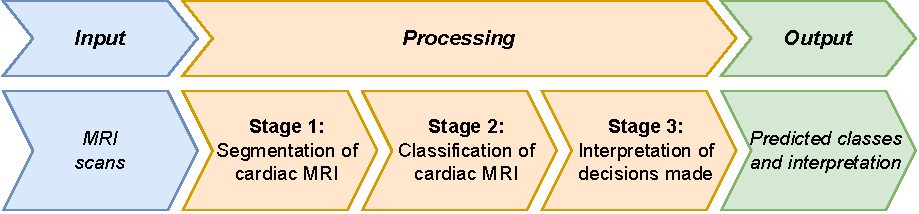
\includegraphics[width=0.8\linewidth]{img/56_fig_1_methods_chart.pdf}
\caption{The proposed task decomposition for cardiac MRI processing, illustrating the process flow from input MRI scans through three sequential processing stages—segmentation, classification, and interpretation of decisions—resulting in the output of predicted classes and interpretations.}
\label{fig:task_decomposition}
\end{figure}

This decomposition is motivated by the following considerations.

\begin{enumerate}
    \item Instead of analyzing the entire cardiac MRI scan, focus on the localized and segmented areas that are relevant for analysis (RV, LV, and myocardium). This enables the DL model to concentrate on essential regions rather than extraneous information. Isolating this function as a separate task allows for selecting specialized DL models best suited for such preprocessing.
    \item Medical datasets for classifier training often have limited sample sizes, making it challenging to achieve sufficient model generalization for multiple classes. Class confusion is common. Many approaches have been proposed to address this issue, including data augmentation. Using a cascade of separate binary classifiers for aggregated classes allows the model to increase the number of samples per aggregated class and focus on specific features of two aggregated classes simultaneously, leading to higher classification accuracy.
    \item In the medical domain, the problem of interpretability of AI models is particularly critical. Addressing this issue is essential to overcome the “black box” effect, which undermines trust in clinical AI outcomes. This study proposes presenting DL-based results in a physician-friendly format through clinically familiar features.
\end{enumerate}

The following sections provide a more detailed description of each method proposed to solve these decomposed tasks.

\subsection*{Method of Multi-Stage Cardiac MRI Segmentation}

At first, the idea of the method was initially approbated at the Informatics \& Data-Driven Medicine (IDDM-2023) conference \cite{Slobodzian:2024}.

In this study, an original dataset, extracted from the ACDC dataset and denoted \({D_1},\) contains pairs of MRI scans and physician-created masks covering three cardiac regions of interest—(i) LV, (ii) RV, and (iii) Mo:
\begin{equation}
    {D_1} = \{ {\mkern 1mu} {d_1},{\mkern 1mu} {d_2}, \ldots ,{d_N}\} ,\quad {d_i} = ({\rm{Im}}{{\rm{g}}_i},{\mkern 1mu} {\rm{Ms}}{{\rm{k}}_i}),\quad {\kern 1pt} i = 1,2, \ldots ,N,
\end{equation}

where \({\rm{Im}}{{\rm{g}}_i}\) is the cardiac MRI scan, \({\rm{Ms}}{{\rm{k}}_i}\) is its corresponding mask, and N is the total number of pairs.

Existing solutions train a single DL model on \({D_1}\) per equation (1) to detect all three regions at once. However, studies \cite{Wehbe:2023,Pandey:2023} suggest specialized DL models can yield more precise results. Accordingly, this research proposes:

\begin{itemize}
    \item Prelocalizing (detecting) LV, RV, and myocardium areas on the MRI scan.
    \item Using three separate masks instead of a single multistructure one.
\end{itemize}

We hypothesize that these changes improve segmentation accuracy. Therefore, we introduce six DL models:

\begin{itemize}
    \item \({M_1}\), \({M_2}\), \({M_3}\): localize LV, RV, and myocardium, respectively.
    \item \({M_4}\), \({M_5}\), \({M_6}\): refine the contours (masks) for each of those regions.
\end{itemize}

For \({M_1}\), \({M_2}\), \({M_3}\), we utilize U-Net with a ResNet-50 encoder; for \({M_4}\), \({M_5}\), \({M_6},\) the same approach but with ResNet-34. In both cases, training requires adapted datasets derived from \({D_1}\).
The models were implemented using the \texttt{segmentation\_models.pytorch} library v0.3.3 with a FastAI v2.7.13 wrapper, employing standard, well-established architectures to ensure reproducibility. For the localization models (\({M_1}\)–\({M_3}\)), a U-Net with a ResNet-50 encoder pre-trained on ImageNet was used, while the segmentation models (\({M_4}\)–\({M_6}\)) used a ResNet-34 encoder. No novel modifications were made to the U-Net framework itself; the primary architectural changes were adapting the first convolutional layer to accept single-channel grayscale inputs and modifying the final output layer for binary segmentation (one class). The models were trained end-to-end, with the total number of trainable parameters being approximately 31.1 million for the U-Net with a ResNet-50 encoder (input size 256×256) and 24.5 million for the U-Net with a ResNet-34 encoder (input size 64×64). Our contribution lies not in a novel network architecture but in the strategic decomposition of the segmentation task and the optimized application of existing architectures for cardiac analysis.

A second dataset \({D_2}\) is defined to train \({M_1}\), \({M_2}\), \({M_3}\):
\begin{equation}
    {D_2} = \{ {\mkern 1mu} {d_1},{\mkern 1mu} {d_2}, \ldots ,{d_N}\} ,\quad {d_i} = ({\rm{ctIm}}{{\rm{g}}_i},{\mkern 1mu} {\rm{ctMsk}}_i^1,{\mkern 1mu} {\rm{ctMsk}}_i^2,{\mkern 1mu} {\rm{ctMsk}}_i^3),
\end{equation}

where \({\rm{ctIm}}{{\rm{g}}_i}\) is the cropped cardiac MRI, while \({\rm{ctMsk}}_i^1,\) \({\rm{ctMsk}}_i^2,\) \({\rm{ctMsk}}_i^3\) are its three cropped masks.
All images in dataset \({D_2}\) per equation (2) are resized to a uniform resolution. Original masks \({\rm{Ms}}{{\rm{k}}_i}\) from \({D_1}\) are decomposed into separate LV, RV, and myocardium masks.

For \({M_4}\), \({M_5}\), \({M_6}\), three further datasets \({D_3}\), \({D_4}\), \({D_5}\) are formed:
\begin{equation}
    {D_3} = \{ {\mkern 1mu} {d_1},{\mkern 1mu} \ldots ,{d_N}\} ,\quad {d_i} = ({\rm{lvIm}}{{\rm{g}}_i},{\mkern 1mu} {\rm{lvMs}}{{\rm{k}}_i}),
\end{equation}

\begin{equation}
    {D_4} = \{ {\mkern 1mu} {d_1},{\mkern 1mu} \ldots ,{d_N}\} ,\quad {d_i} = ({\rm{rvIm}}{{\rm{g}}_i},{\mkern 1mu} {\rm{rvMs}}{{\rm{k}}_i}),
\end{equation}

\begin{equation}
    {D_5} = \{ {\mkern 1mu} {d_1},{\mkern 1mu} \ldots ,{d_N}\} ,\quad {d_i} = ({\rm{myoIm}}{{\rm{g}}_i},{\mkern 1mu} {\rm{myoMs}}{{\rm{k}}_i}).
\end{equation}

Each dataset formalized by equations (3)–(5) localizes and centers images/masks around one structure, adding a 15\% margin. After segmentation, images must revert to original dimensions for final validation, possibly causing detail loss. To address this, Gaussian smoothing is utilized as suggested in our previous work \cite{Slobodzian:2024}—balancing quality and computational cost better than other filters. The parameter \(\sigma \) is selected via grid search on a validation split of the training data and then fixed for all test set inferences.

Thus, the task of obtaining DL models for subsequent segmentation of regions of interest in an MRI scan is presented through the following steps of the method (Figure \ref{fig:dl_models_segmentation}).

\begin{figure}[ht]
\centering
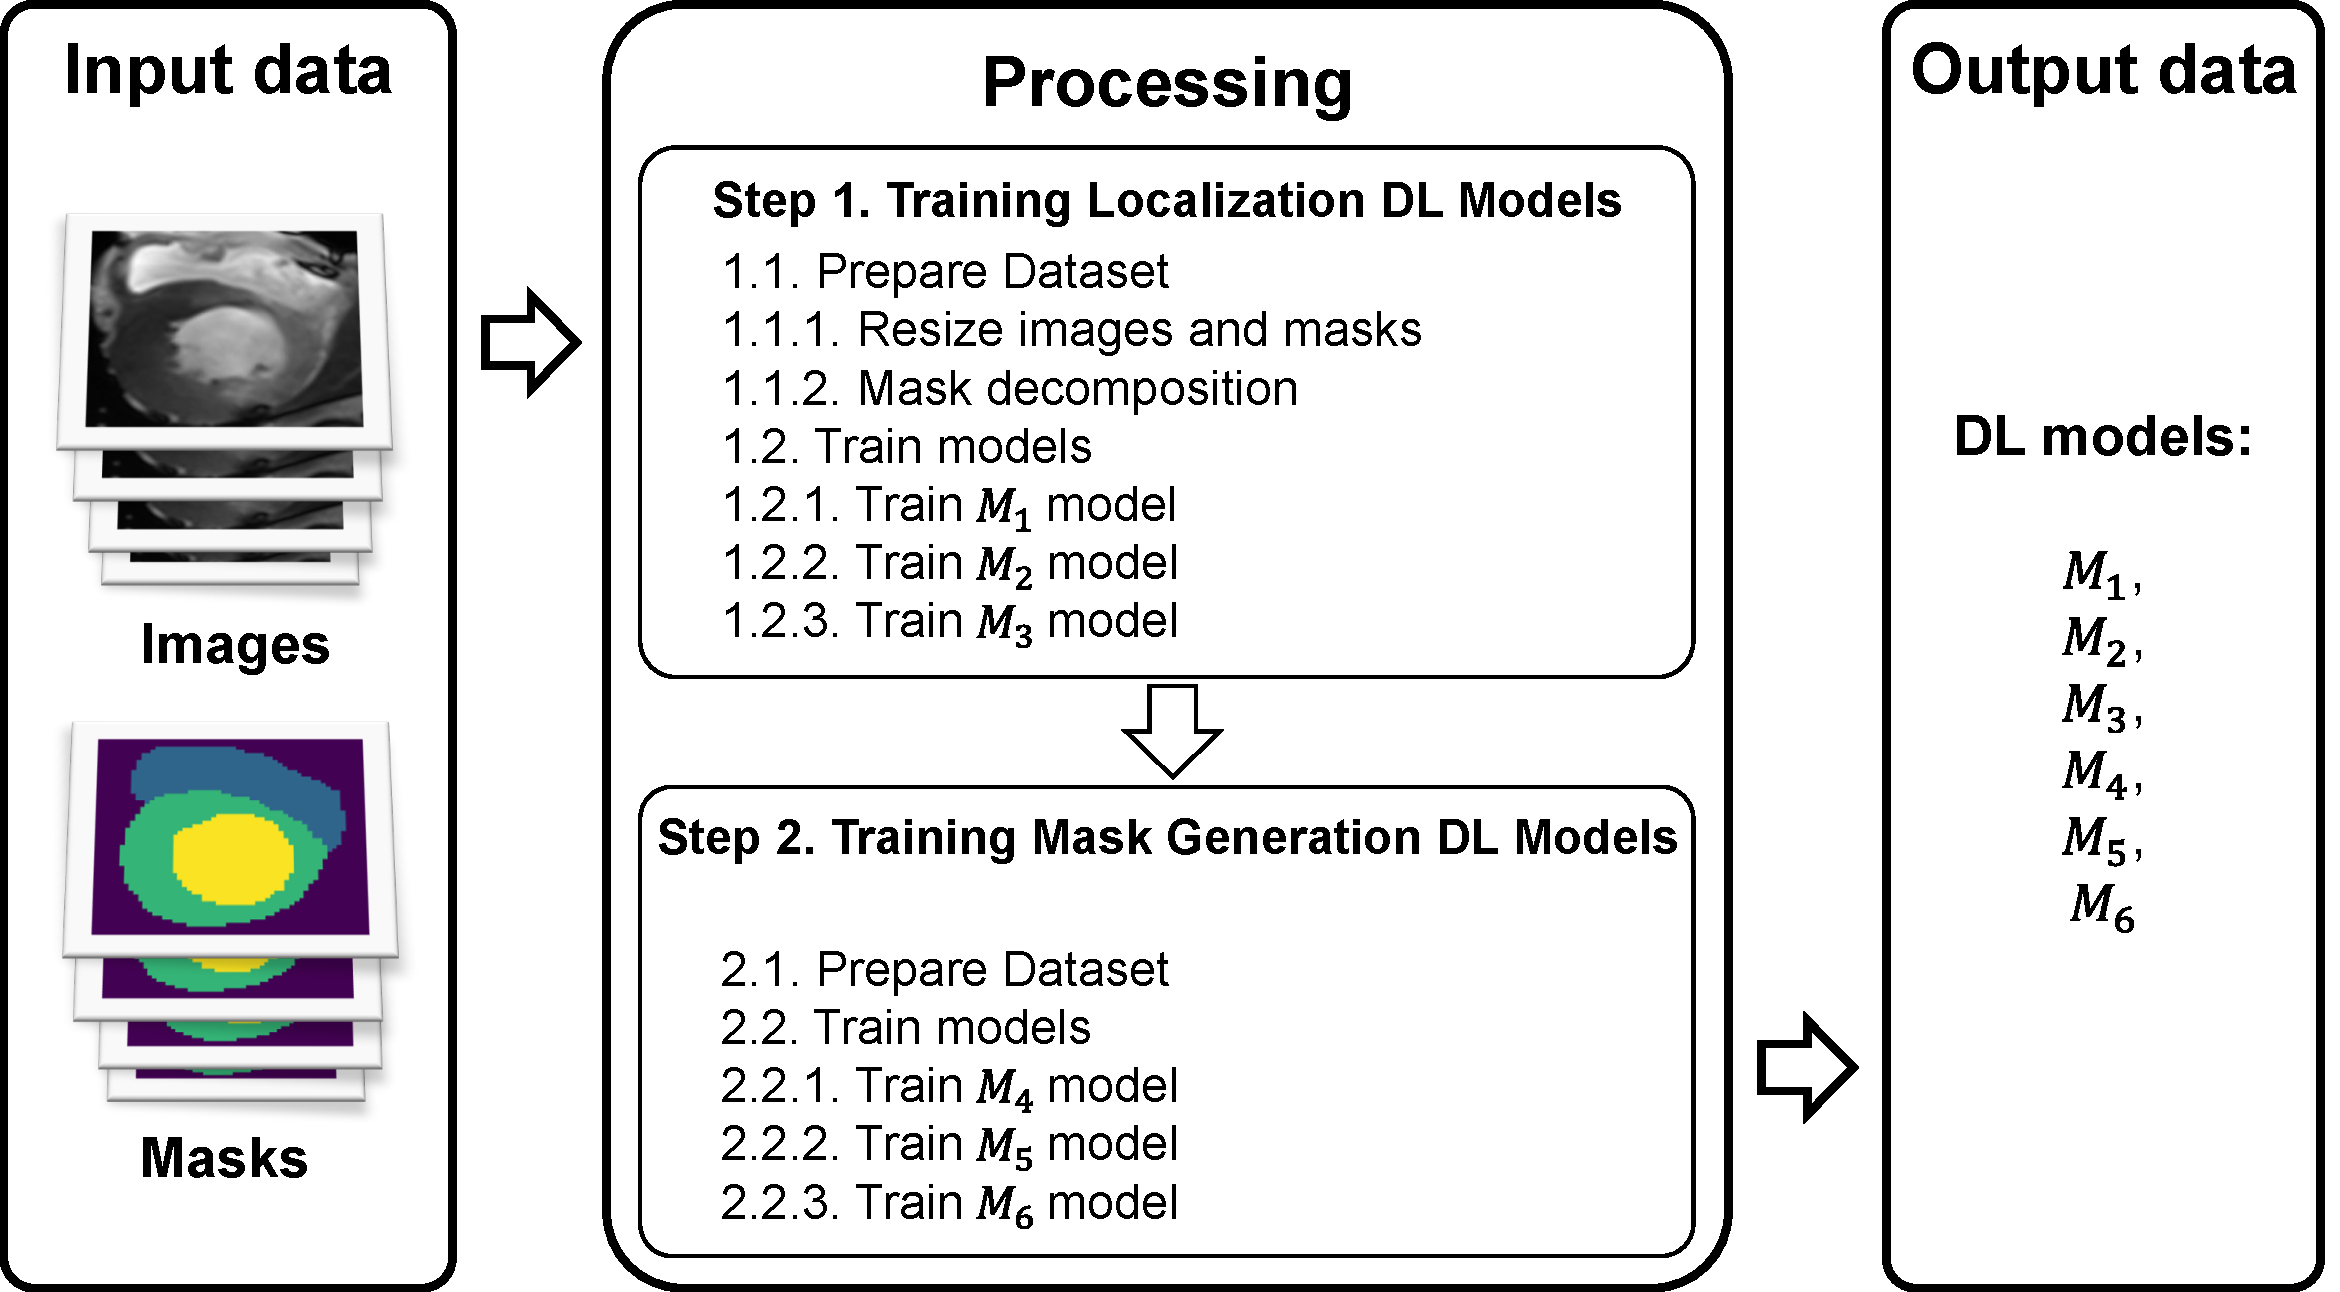
\includegraphics[width=0.8\linewidth]{img/56_fig_2_train-segment.pdf}
\caption{The main steps for obtaining DL models for segmenting the LV, RV, and myocardium regions in an MRI scan.}
\label{fig:dl_models_segmentation}
\end{figure}

The procedure for creating the DL models for MRI scan segmentation involves several data preparation steps and the training of six distinct models, as summarized in Algorithm~\ref{alg:training}. The input data is a subset \({D_1}\) of \cite{Bernard:2018}, containing pairs of MRI scans and corresponding masks with regions of the LV, RV, and LV myocardium.

\begin{algorithm}[ht]
\caption{Training Procedure for Segmentation Models}\label{alg:training}
\begin{algorithmic}[1]
\Require Original dataset $D_1 = \{(\text{Img}_i, \text{Msk}_i)\}_{i=1}^N$
\Ensure Trained models $M_1, \dots, M_6$
\State \textbf{Function} PrepareLocalizationData($D_1$):
\State $D_2 \gets \emptyset$
\ForAll{$(\text{Img}_i, \text{Msk}_i) \in D_1$}
    \State $\text{Img}_i' \gets \text{Resize}(\text{Img}_i, (256, 256))$
    \State $\text{Msk}_i' \gets \text{Resize}(\text{Msk}_i, (256, 256))$
    \State $(\text{Msk}_i^{\text{LV}}, \text{Msk}_i^{\text{RV}}, \text{Msk}_i^{\text{Myo}}) \gets \text{DecomposeMask}(\text{Msk}_i')$
    \State Add $(\text{Img}_i', \text{Msk}_i^{\text{LV}}, \text{Msk}_i^{\text{RV}}, \text{Msk}_i^{\text{Myo}})$ to $D_2$
\EndFor
\State \textbf{return} $D_2$

\State \textbf{Function} PrepareSegmentationData($D_1$):
\State $D_3, D_4, D_5 \gets \emptyset, \emptyset, \emptyset$
\ForAll{$(\text{Img}_i, \text{Msk}_i) \in D_1$}
    \State $(\text{lvImg}_i, \text{lvMsk}_i) \gets \text{CropAndResize}(\text{Img}_i, \text{Msk}_i, \text{region='LV'})$
    \State Add $(\text{lvImg}_i, \text{lvMsk}_i)$ to $D_3$
    \State $(\text{rvImg}_i, \text{rvMsk}_i) \gets \text{CropAndResize}(\text{Img}_i, \text{Msk}_i, \text{region='RV'})$
    \State Add $(\text{rvImg}_i, \text{rvMsk}_i)$ to $D_4$
    \State $(\text{myoImg}_i, \text{myoMsk}_i) \gets \text{CropAndResize}(\text{Img}_i, \text{Msk}_i, \text{region='Myo'})$
    \State Add $(\text{myoImg}_i, \text{myoMsk}_i)$ to $D_5$
\EndFor
\State \textbf{return} $D_3, D_4, D_5$

\State $D_2 \gets \text{PrepareLocalizationData}(D_1)$
\State $M_1 \gets \text{TrainModel}(\text{U-Net-ResNet50 on } D_2, \text{target='LV'})$
\State $M_2 \gets \text{TrainModel}(\text{U-Net-ResNet50 on } D_2, \text{target='RV'})$
\State $M_3 \gets \text{TrainModel}(\text{U-Net-ResNet50 on } D_2, \text{target='Myo'})$

\State $D_3, D_4, D_5 \gets \text{PrepareSegmentationData}(D_1)$
\State $M_4 \gets \text{TrainModel}(\text{U-Net-ResNet34 on } D_3, \text{target='LV'})$
\State $M_5 \gets \text{TrainModel}(\text{U-Net-ResNet34 on } D_4, \text{target='RV'})$
\State $M_6 \gets \text{TrainModel}(\text{U-Net-ResNet34 on } D_5, \text{target='Myo'})$
\end{algorithmic}
\end{algorithm}

In Step 1, DL models are trained to localize the regions of the LV, RV, and myocardium. Specifically, in Step 1.1, a new dataset \({D_2}\) is prepared, which contains three masks instead of one: for the LV, RV, and myocardium. This involves the following substeps:

\begin{enumerate}[label=Step 1.1.\arabic*:, leftmargin=6.5em]
    \item Resizing all input images and masks to a uniform size.
    \item Decomposing the original mask into separate masks for the LV, RV, and myocardium.
\end{enumerate}

Thus, the new dataset \({D_2}\) contains rows containing an MRI scan and three masks.

Next, in Step 1.2, using dataset \({D_2}\), three DL models are trained to detect the regions of interest as follows:

\begin{enumerate}[label=Step 1.2.\arabic*:, leftmargin=6.5em]
    \item Training DL model \({M_1}\) to detect the LV region.
    \item Training DL model \({M_2}\) to detect the RV region.
    \item Training DL model \({M_3}\) to detect the myocardium region.
\end{enumerate}

In Step 2, DL models are trained to generate masks based on the detected regions of interest. In Step 2.1, new datasets \({D_3}\), \({D_4}\), and \({D_5}\) are prepared by modifying dataset \({D_2}\), specifically by cropping the original MRI scans and masks according to the regions of interest.

Subsequently, in Step 2.2, using datasets \({D_3}\), \({D_4}\), and \({D_5}\), three DL models are trained to delineate the contours of the LV, RV, and myocardium:

\begin{enumerate}[label=Step 2.2.\arabic*:, leftmargin=6.5em]
    \item Training DL model \({M_4}\) to delineate the LV contours using dataset \({D_3}\).
    \item Training DL model \({M_5}\) to delineate the RV contours using dataset \({D_4}\).
    \item Training DL model \({M_6}\) to delineate the myocardium contours using dataset \({D_5}\).
\end{enumerate}

The output data consists of the trained DL models \({M_1}\), \({M_2}\), \({M_3}\), \({M_4}\), \({M_5}\), \({M_6}\).

The inference process for segmenting an arbitrary MRI scan uses the trained deep learning models (\(M_1\)–\(M_6\)) to sequentially localize the cardiac structures, generate precise masks, and perform post-processing. This multi-stage workflow, which ensures high precision by breaking the task into specialized steps, is illustrated in Figure~\ref{fig:mri_scan_segmentation} and detailed in Algorithm~\ref{alg:inference}. The input data consists of an MRI scan and the six trained DL models.

\begin{figure}[ht]
    \centering
    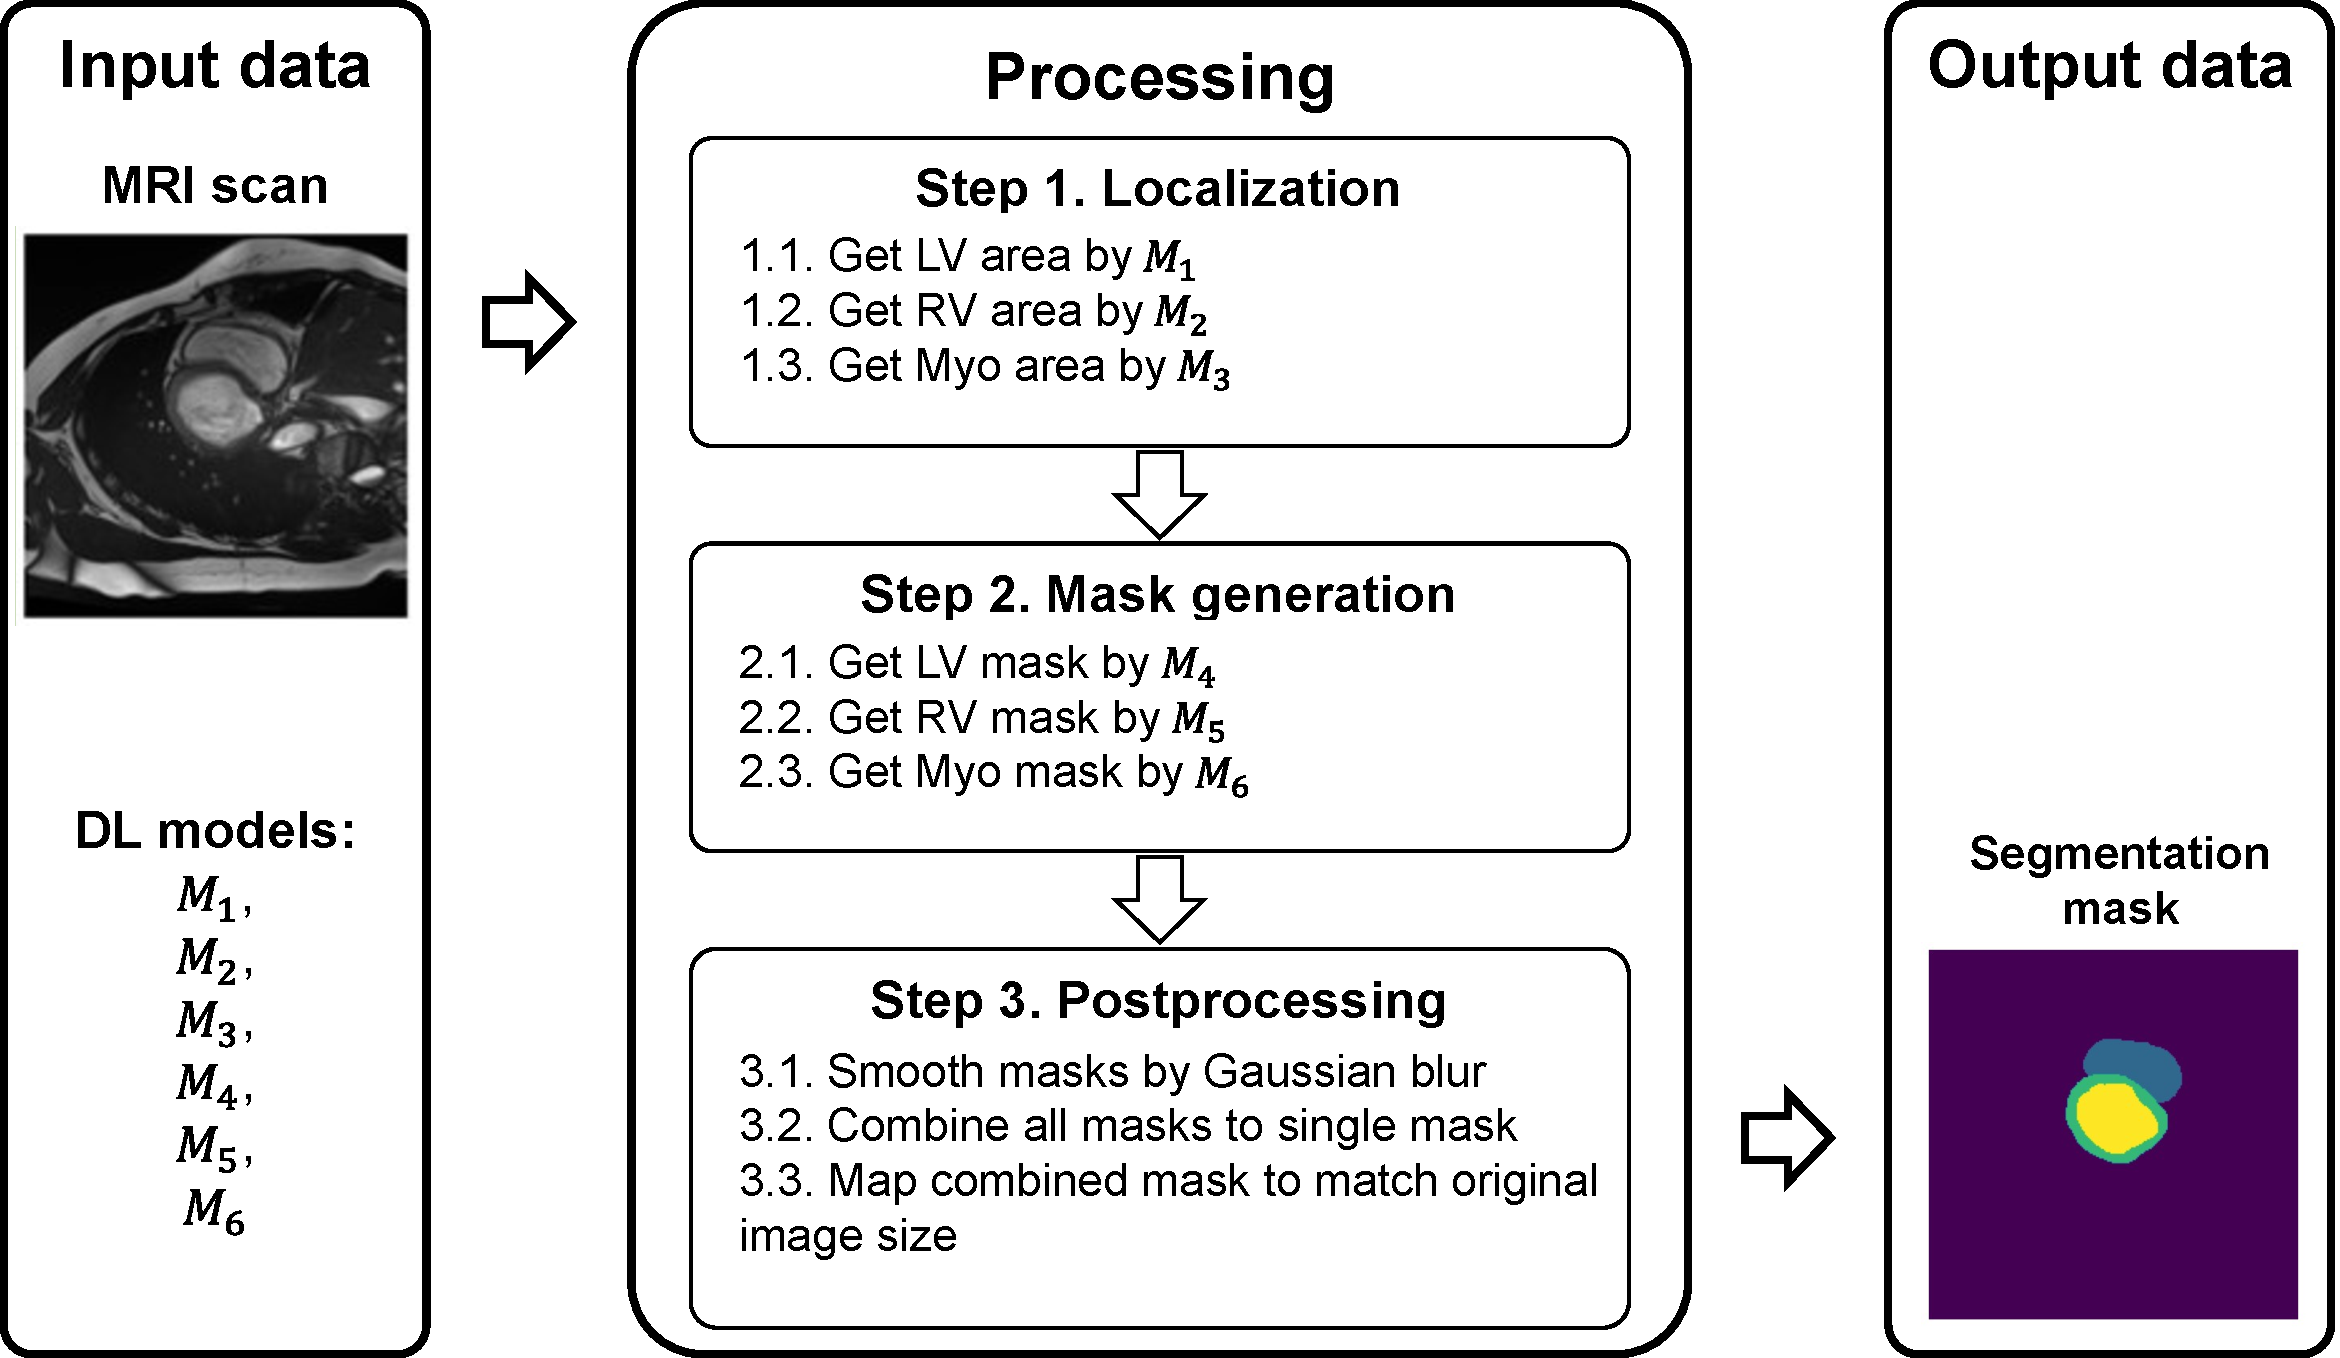
\includegraphics[width=0.8\linewidth]{img/56_fig_3_method-segment.pdf}
    \caption{The main steps for segmenting an MRI scan into regions of the LV, RV, and myocardium.}
    \label{fig:mri_scan_segmentation}
\end{figure}

\begin{algorithm}[ht]
    \caption{Inference Procedure for Multi-Stage Segmentation}\label{alg:inference}
    \begin{algorithmic}[1]
    \Require Arbitrary MRI scan Img, Trained models $M_1, \dots, M_6$
    \Ensure Final segmented mask $\text{FinalMsk}$
    \Statex
    \State $\text{OriginalSize} \gets \text{GetSize}(\text{Img})$
    \State $\text{Img}' \gets \text{Resize}(\text{Img}, (256, 256))$
    \Statex
    \State \textit{// Step 1: Localize ROI bounding boxes}
    \State $\text{bbox}_{\text{LV}} \gets M_1(\text{Img}')$
    \State $\text{bbox}_{\text{RV}} \gets M_2(\text{Img}')$
    \State $\text{bbox}_{\text{Myo}} \gets M_3(\text{Img}')$
    \Statex
    \State \textit{// Step 2: Generate masks for localized regions}
    \State $\text{Crop}_{\text{LV}} \gets \text{CropImage}(\text{Img}, \text{bbox}_{\text{LV}})$
    \State $\text{PredMsk}_{\text{LV}} \gets M_4(\text{Crop}_{\text{LV}})$
    \State $\text{Crop}_{\text{RV}} \gets \text{CropImage}(\text{Img}, \text{bbox}_{\text{RV}})$
    \State $\text{PredMsk}_{\text{RV}} \gets M_5(\text{Crop}_{\text{RV}})$
    \State $\text{Crop}_{\text{Myo}} \gets \text{CropImage}(\text{Img}, \text{bbox}_{\text{Myo}})$
    \State $\text{PredMsk}_{\text{Myo}} \gets M_6(\text{Crop}_{\text{Myo}})$
    \Statex
    \State \textit{// Step 3: Post-process and combine masks}
    \State $\text{SmoothMsk}_{\text{LV}} \gets \text{GaussianBlur}(\text{PredMsk}_{\text{LV}})$
    \State $\text{SmoothMsk}_{\text{RV}} \gets \text{GaussianBlur}(\text{PredMsk}_{\text{RV}})$
    \State $\text{SmoothMsk}_{\text{Myo}} \gets \text{GaussianBlur}(\text{PredMsk}_{\text{Myo}})$
    \Statex
    \State $\text{CombinedMsk} \gets \text{Combine}(\text{SmoothMsk}_{\text{LV}}, \text{SmoothMsk}_{\text{RV}}, \text{SmoothMsk}_{\text{Myo}})$
    \State $\text{FinalMsk} \gets \text{Resize}(\text{CombinedMsk}, \text{OriginalSize})$
    \State \textbf{return} $\text{FinalMsk}$
    \end{algorithmic}
\end{algorithm}

Next, we describe the steps for segmenting an MRI scan into regions of the LV, RV, and myocardium.

The input data consists of an MRI scan and the DL models \({M_1}\), \({M_2}\), \({M_3}\), \({M_4}\), \({M_5}\), and \({M_6}\).

\begin{enumerate}[label=Step \arabic*:, leftmargin=5em]
    \item Determine the locations of the LV, RV, and myocardium regions:
    \begin{enumerate}[label=Step 1.\arabic*:, leftmargin=2.5em]
        \item Using DL model \({M_1}\), determine the location of the LV.
        \item Using DL model \({M_2}\), determine the location of the RV.
        \item Using DL model \({M_3}\), determine the location of the myocardium.
    \end{enumerate}
    \item Generate masks for the LV, RV, and myocardium:
    \begin{enumerate}[label=Step 2.\arabic*:, leftmargin=2.5em]
        \item Using DL model \({M_4}\), generate the mask for the LV.
        \item Using DL model \({M_5}\), generate the mask for the RV.
        \item Using DL model \({M_6}\), generate the mask for the myocardium.
    \end{enumerate}
    \item Perform postprocessing of the obtained masks:
    \begin{enumerate}[label=Step 3.\arabic*:, leftmargin=2.5em]
        \item Smoothing the masks.
        \item Combining the three individual masks into a single comprehensive mask.
        \item Mapping the combined mask to match the size of the input image.
    \end{enumerate}
\end{enumerate}

The output of the method is a segmented arbitrary MRI heart image into regions of the LV, RV, and myocardium.

Thus, the process of constructing DL models includes data preparation and training models for localization and mask generation of regions of interest using modified datasets. Separate models are trained for localizing and delineating the contours of the LV, RV, and myocardium. In total, six DL models were trained.

MRI scan segmentation is performed sequentially: first, the models determine the locations of the LV, RV, and the myocardium regions, after which the corresponding masks are generated. The final step is postprocessing the masks, which includes smoothing, combining, and adapting them to the size of the input image. The result is a segmented MRI heart image.

\Rtwo{\revtag{2}{2}\subsection*{Apical/Basal Refinement}}
\Rtwo{\revtag{2}{6} % Action 5 & 6
We introduce a slice-position-aware refinement module to improve segmentation accuracy on apical and basal slices, where boundary delineation is notoriously challenging due to partial volume effects and anatomical ambiguity. This module, applied after the initial segmentation, incorporates two components: (i) a shape-prior loss that uses signed-distance transforms derived from the training masks to penalize anatomically implausible contours, and (ii) a 3D continuity penalty that encourages smooth transitions between neighboring slices. This refinement specifically targets under- and over-segmentation errors common at the ventricular extremes. We report Dice scores stratified by basal, mid-ventricular, and apical slice locations to quantify the module's impact.
}

\subsection*{Method of Cardiac MRIs Cascade Classification}

The idea of this method was originally presented at the Information Technology and Implementation (IT\&I-2024) conference \cite{Slobodzian:2025}.

This study focuses on four pathologies in MRI scans: DCM, HCM, MINF, ARV, including normal state denoted NOR. The proposed method includes the following:

\begin{itemize}
    \item Accounting for anatomic heart parameters via certain modifications of an input MRI.
    \item Using both diastolic and systolic MRI phases.
    \item A cascade classification model.
    \item A custom DL architecture.
\end{itemize}

Heart pathologies often depend on tissue density, chamber volumes, and myocardial thickness over time. We use segmentation masks obtained by the multi-stage approach to capture geometry and texture. Each structure (LV, RV, and myocardium) is placed in a separate RGB channel, preserving texture in addition to geometry.

Therefore, based on the above considerations, the following decomposition of the input MRI scan is proposed:
\begin{equation}
    F:{I_{MRT}} \to I_{MRT}^{{\rm{new}}},
\end{equation}

\begin{equation}
    I_{MRT}^{{\rm{new}}} = ({\rm{im}}{{\rm{g}}_1}, \ldots ,{\rm{im}}{{\rm{g}}_N}),\quad N = 42,
\end{equation}

where \({\rm{im}}{{\rm{g}}_1} - {\rm{im}}{{\rm{g}}_{21}}\) are systolic short-axis slices, and \({\rm{im}}{{\rm{g}}_{22}} - {\rm{im}}{{\rm{g}}_{42}}\) are diastolic slices.

Images denoted by equation (7) are cropped into bounding boxes that contain all relevant segments. Figure \ref{fig:input_data_visualization} shows the images \({\rm{im}}{{\rm{g}}_i}\) that are fed to the DL model.

\begin{figure}[ht]
\centering
\begin{tabular}{c}
    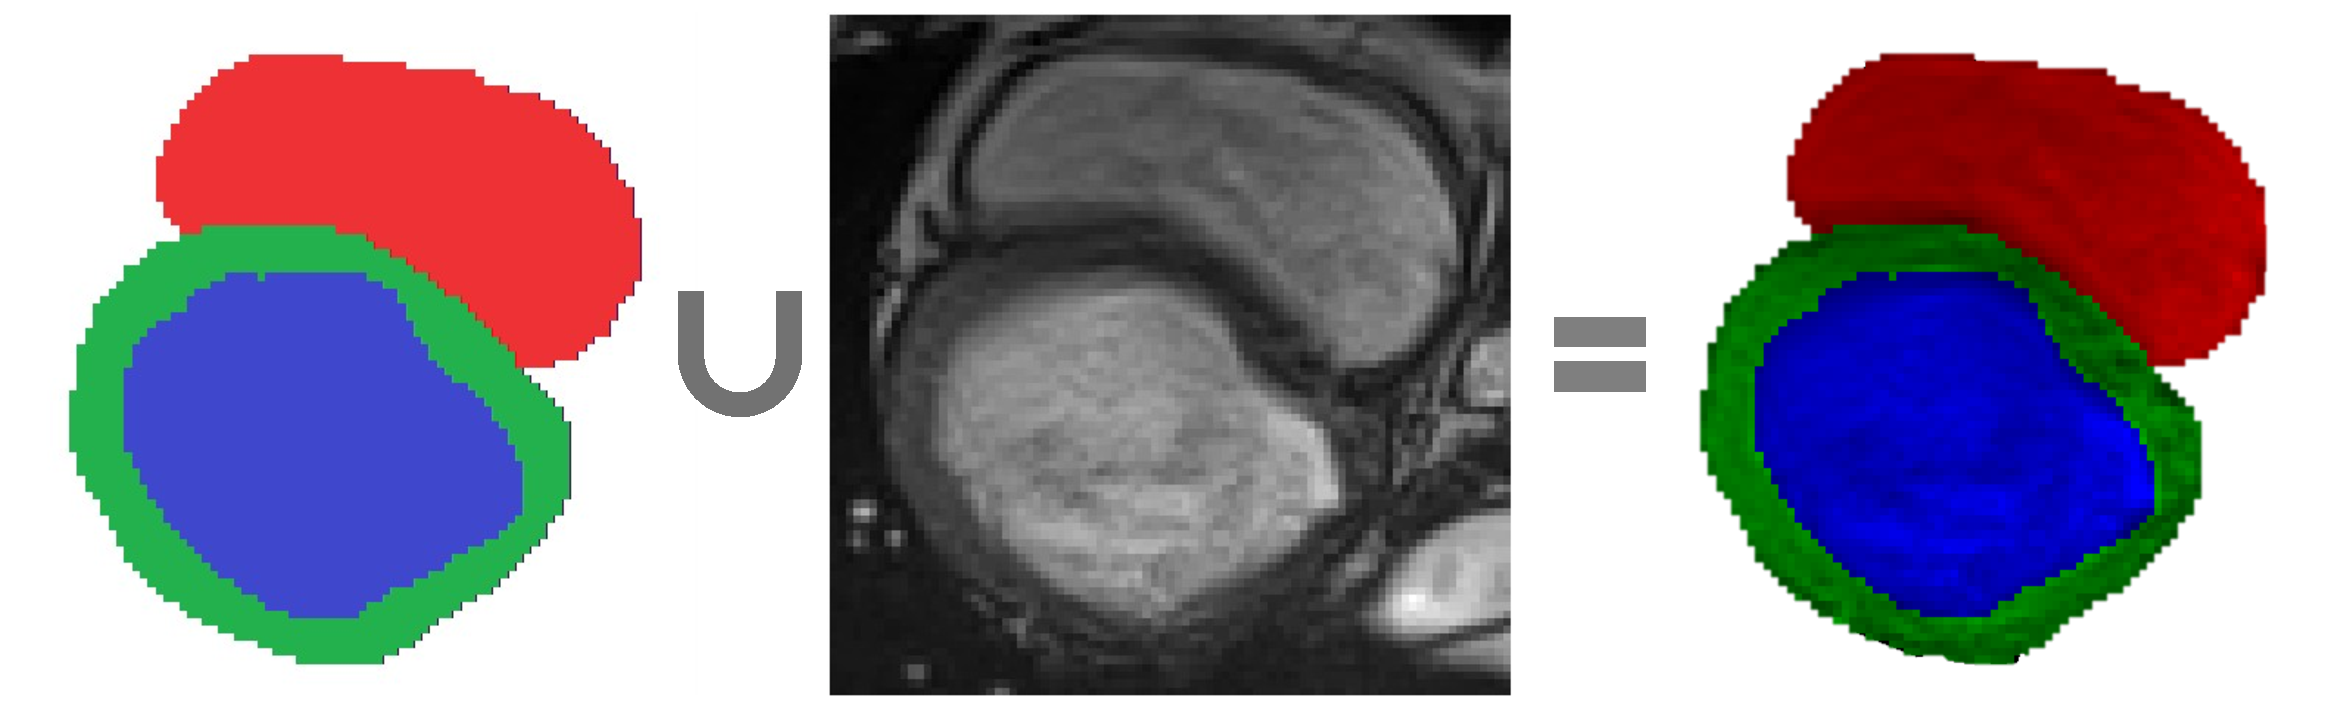
\includegraphics[width=0.4\linewidth]{img/56_fig_4a.pdf} \\
    \textbf{\textsf{(a)}} \\
    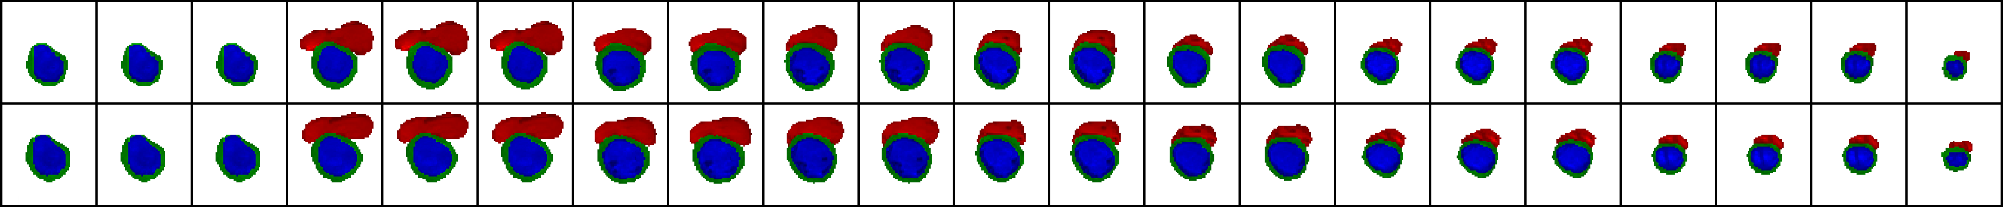
\includegraphics[width=0.9\linewidth]{img/56_fig_4b.pdf} \\
    \textbf{\textsf{(b)}}
\end{tabular}
\caption{This figure illustrates how an MRI is overlaid with color-coded masks to create a combined visualization of the RV (red), LV (blue), and myocardium (green). In \textbf{(a)}, the original MRI is merged with its mask, producing a single superimposed image. In \textbf{(b)}, each column presents short‐axis slices from systolic (top row) and diastolic (bottom row) phases, highlighting all three structures across the cardiac cycle.}
\label{fig:input_data_visualization}
\end{figure}

Based on the representation defined by equation (6), a dataset \({D_6}\) is constructed:
\begin{equation}
    {D_6} = \{ {\mkern 1mu} {d_1}, \ldots ,{d_N}\} ,\quad {d_i} = (I_{MRT}^{{\rm{new}}},{\mkern 1mu} {\rm{Cls}}),
\end{equation}

where \({\rm{Cls}} \in \left\{ {1,2,3,4,5} \right\}\) denotes the pathology class (1 – ARV, 2 – HCM, 3 – MINF, 4 – DCM, 5 – NOR).

Dataset \({D_6}\) is derived from the ACDC dataset, containing systolic and diastolic images for 150 patients in five groups. Some have fewer than 21 short-axis slices; thus, image augmentation is performed by duplicating adjacent slices. \Rthree{\revtag{3}{9}This augmentation occurs only within patient-level training folds to prevent data leakage.}

A cascade classification model is proposed to mitigate class confusion in smaller datasets. We define four binary classifiers (\({M_7}\), \({M_8}\), \({M_9}\), \({M_{10}}\)):

\begin{itemize}
    \item \({M_7}\) – class a – aggregation of classes 1 and 5, class b – aggregation of classes 2, 3, and 4. This model separates all LV pathologies from ARV/NOR – LV pathologies vs. ARV/NOR.
    \item \({M_8}\) – class a – class 1, class b – class 5. \({M_8}\) is aimed to distinguish ARV from NOR, i.e., splits ARV vs. NOR.
    \item \({M_9}\) – class a – class 2, class b – aggregation of classes 3 and 4. It distinguishes ARV from NOR, i.e., splits ARV vs. NOR.
    \item \({M_{10}}\) – class a – class 4, class b – class 3. This model differentiates MINF from DCM.
\end{itemize}

The structure of the proposed cascade classification is shown in Figure \ref{fig:cascade_classification_structure}.

\begin{figure}[ht]
\centering
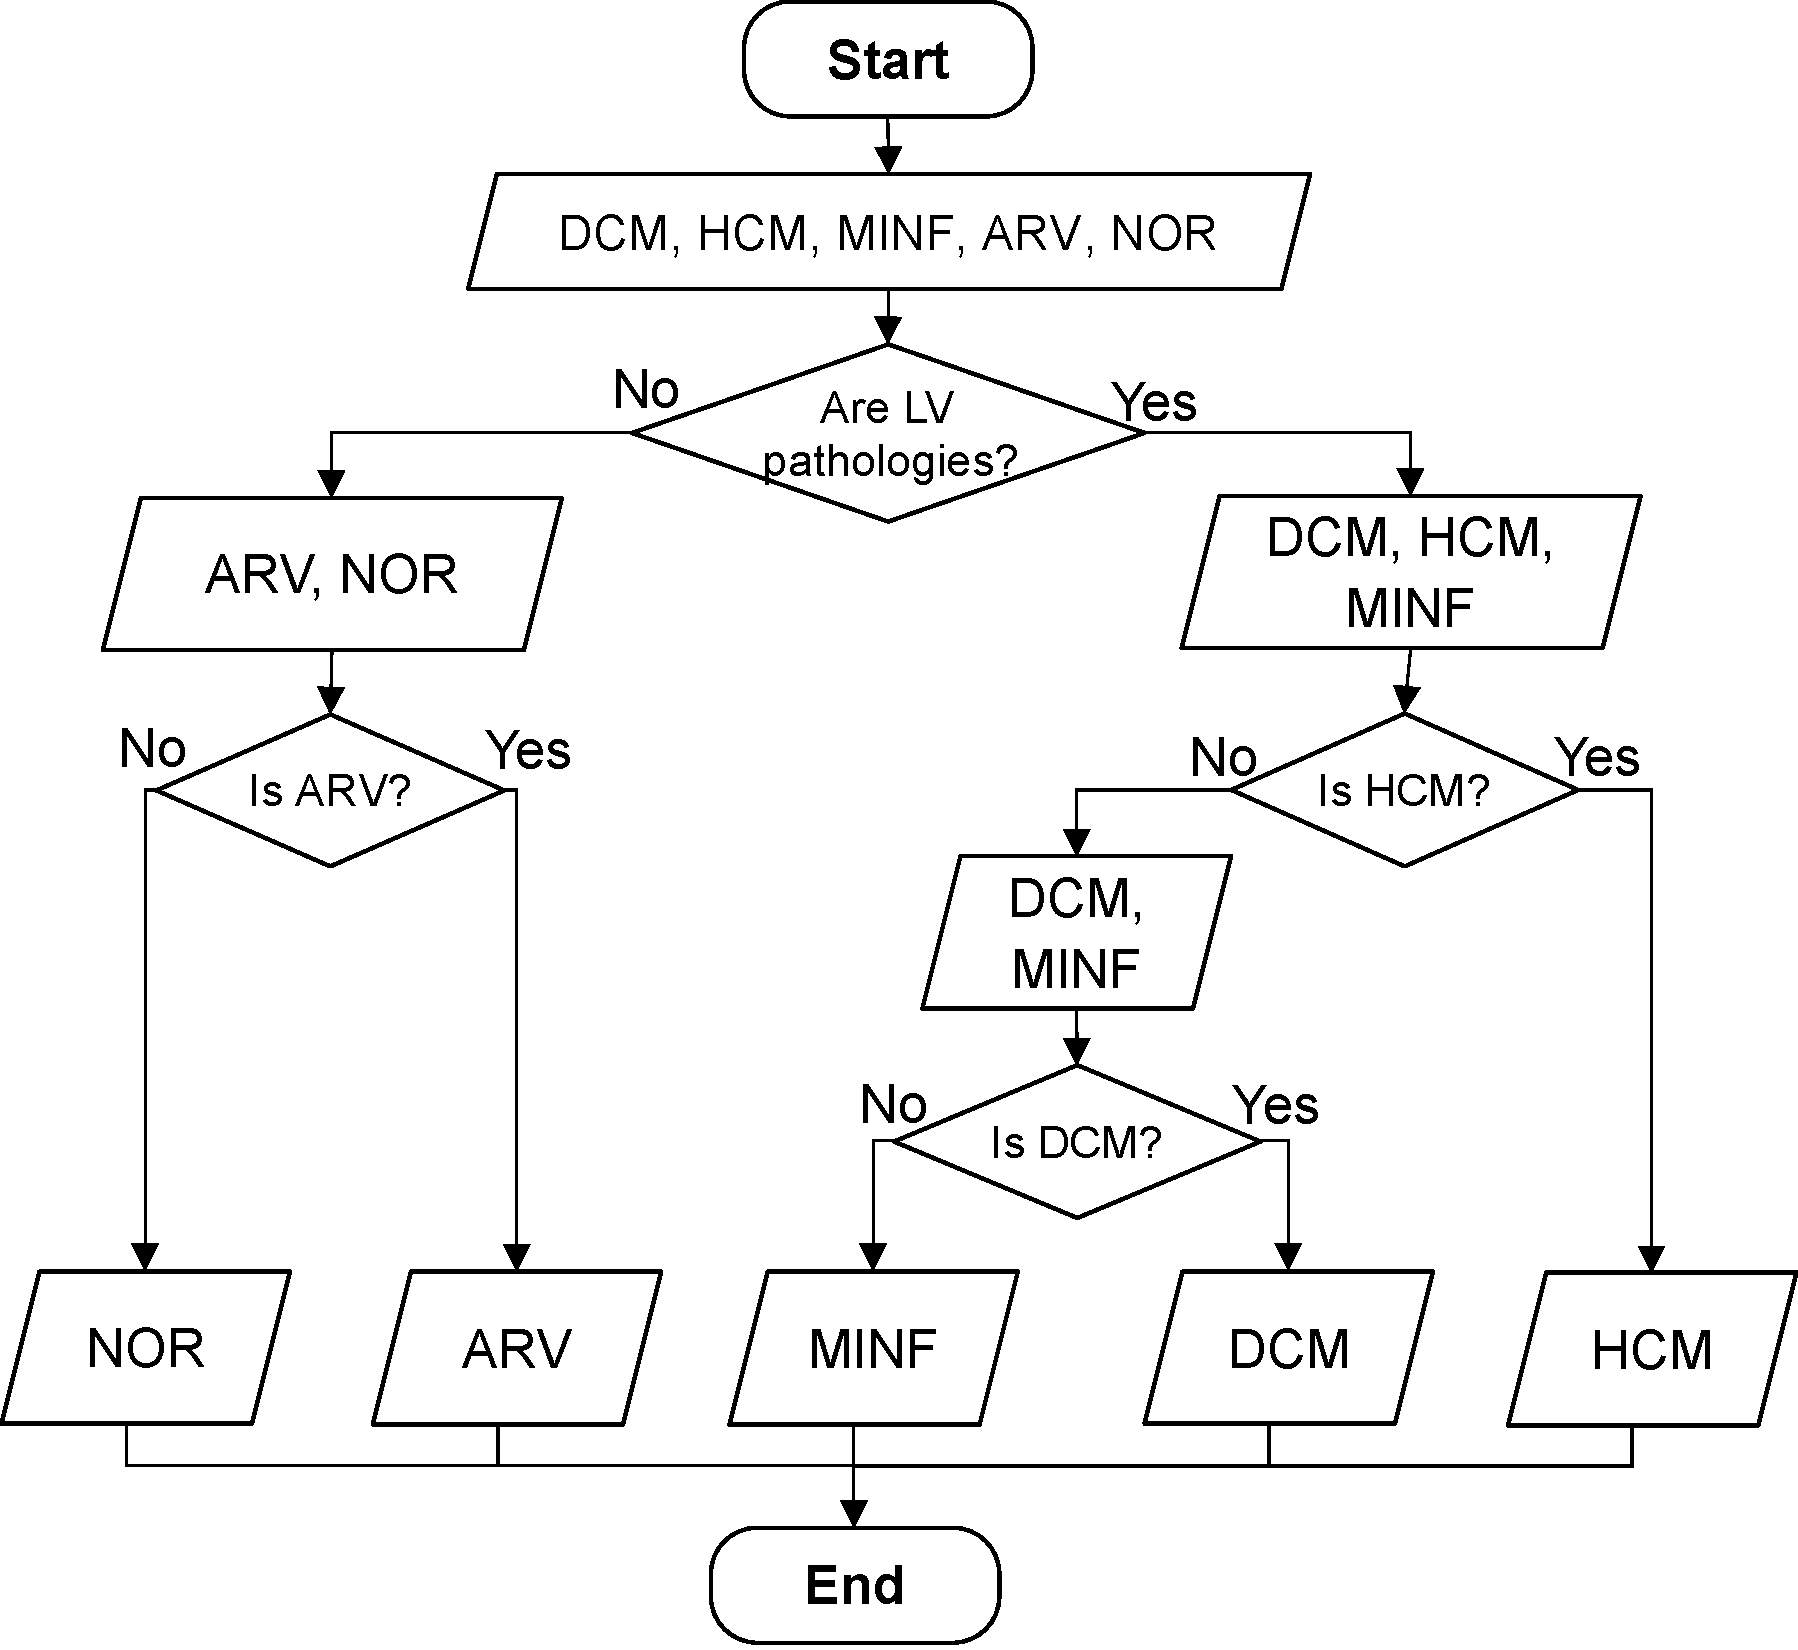
\includegraphics[width=0.6\linewidth]{img/56_fig_5_cascade.pdf}
\caption{Structure of the cascade classification into five classes: ARV, HCM, MINF, DCM, and NOR. Here, LV pathologies are HCM, MINF, and DCM.}
\label{fig:cascade_classification_structure}
\end{figure}

Each model (\({M_7}\), \({M_8}\), \({M_9}\), \({M_{10}}\)) uses a CNN adapted to binary classification, with Adam optimizer and categorical cross entropy as the loss. Adam adaptively adjusts learning rates while cross entropy measures the discrepancy between real labels and predicted probabilities. Early stopping is applied to avoid overfitting, and class proportions are maintained in training and validation splits.

The proposed method consists of two processes: i) training models \({M_7}\), \({M_8}\), \({M_9}\), and \({M_{10}}\) and ii) classifying pathology using an arbitrary cardiac MRI. The overall scheme of this process is illustrated in Figure \ref{fig:training_process_scheme}.

\begin{figure}[ht]
\centering
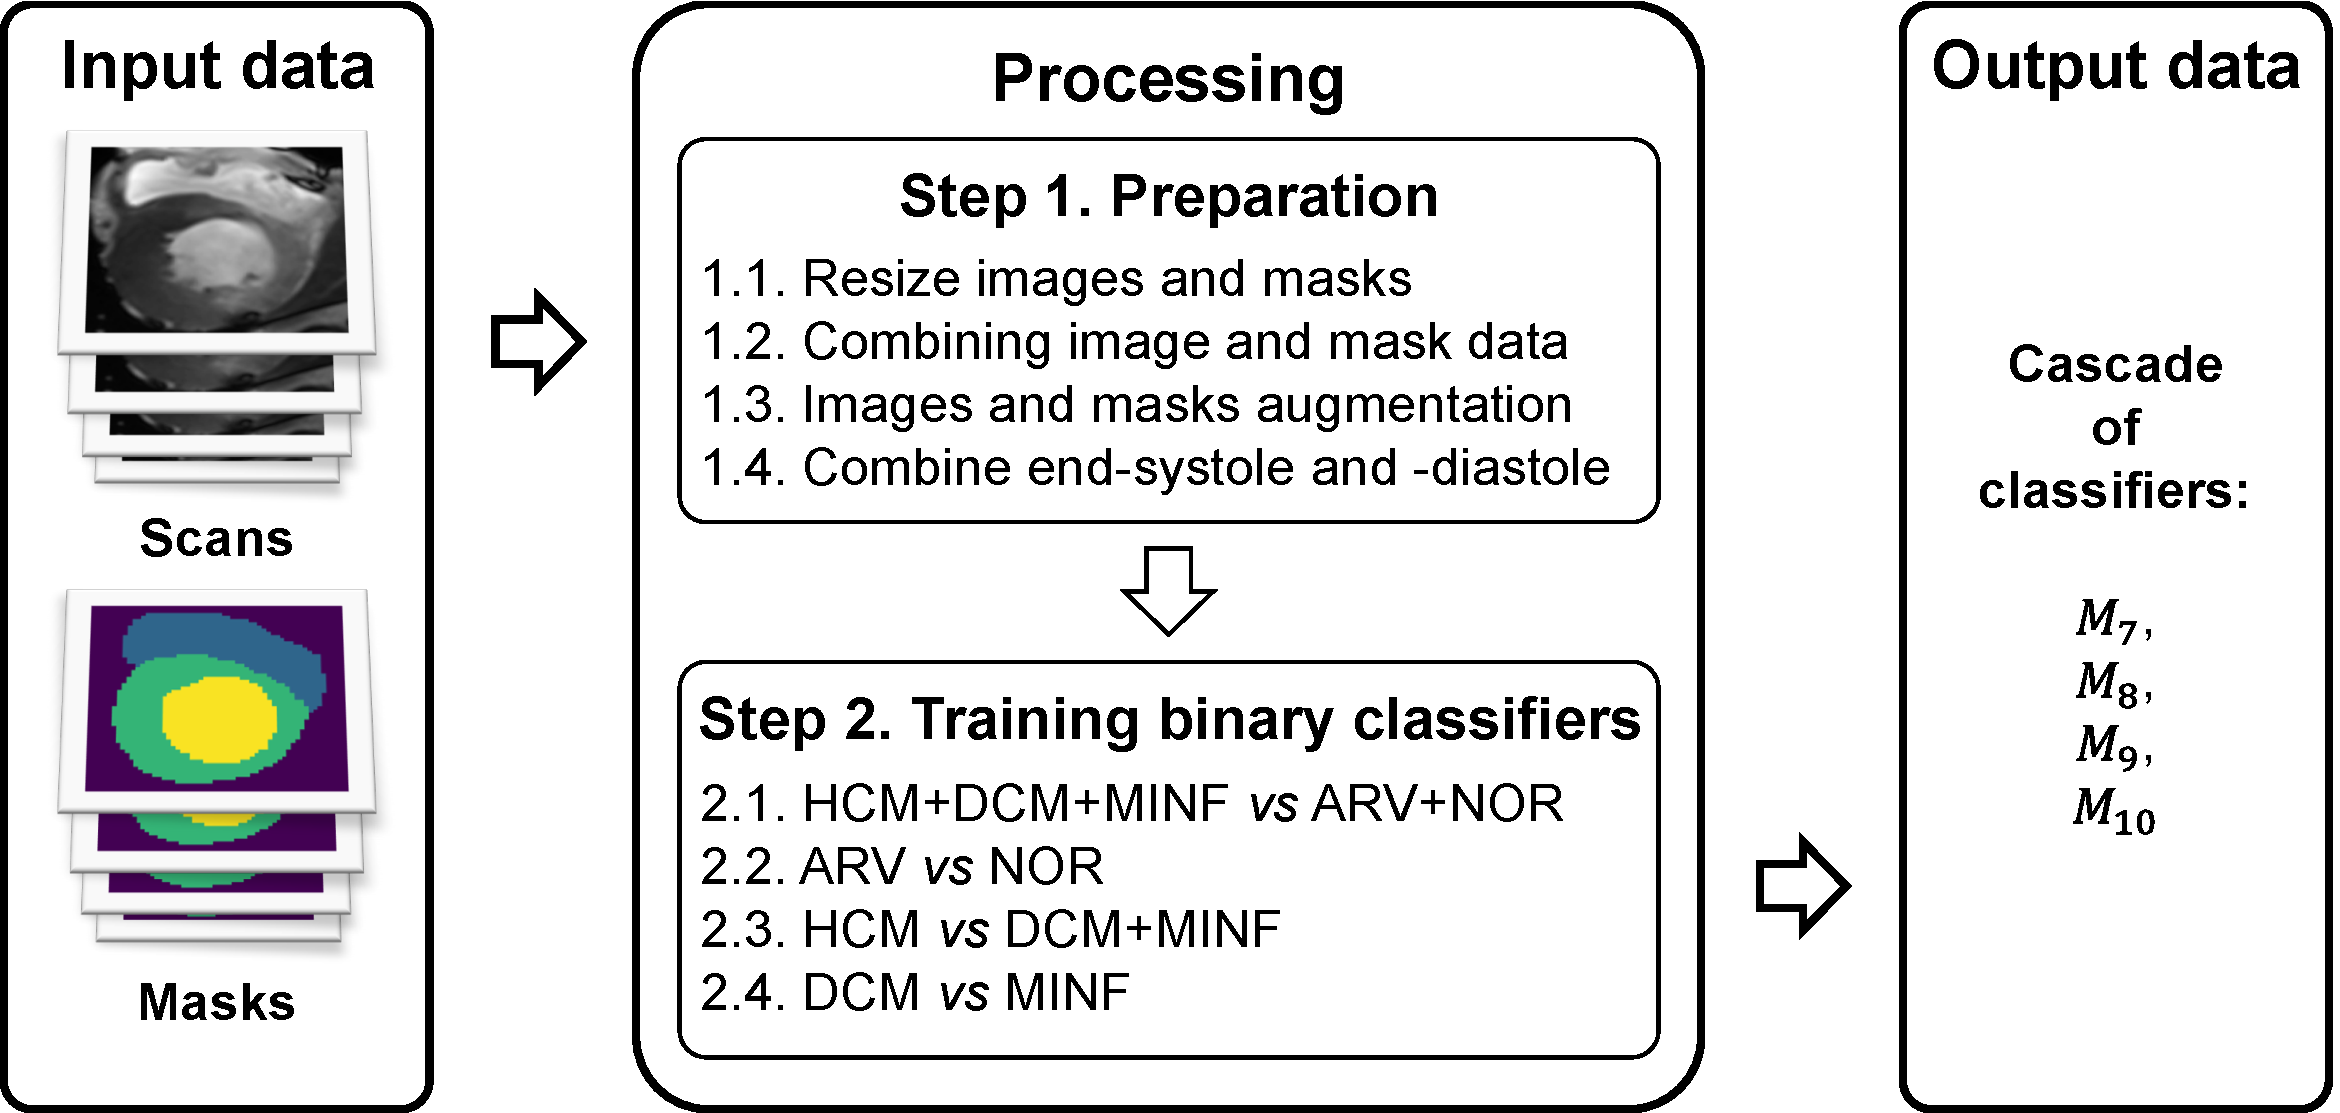
\includegraphics[width=0.8\linewidth]{img/56_fig_6_train-class.pdf}
\caption{Overall scheme of the training process for models \({M_7}\), \({M_8}\), \({M_9}\), and \({M_{10}}\).}
\label{fig:training_process_scheme}
\end{figure}

Below, the main steps of the proposed method are described in detail.
The input data \({D_6}\) consists of images from the ACDC dataset \cite{Bernard:2018}, modified as described above, which contain images for each patient during the diastolic and systolic phases of the cardiac cycle.

\begin{enumerate}[label=Step \arabic*:, leftmargin=5em]
    \item Preparation of MRI scans.
    \begin{enumerate}[label=Step 1.\arabic*:, leftmargin=2.5em]
        \item All MRI scans are cropped to retain only the area with the necessary segments (identified using the first method) and resized to a uniform size.
        \item Mask data and images are combined (each heart segment corresponding to the mask is presented in a separate channel).
        \item Image and mask data are augmented to obtain an equal number of elements for each patient.
        \item Masks and images from the diastolic and systolic phases of the cardiac cycle are combined.
    \end{enumerate}
    \item Training a Cascade of Four Classifiers.
    Each classifier is trained separately using the same approach. The training process begins with creating and compiling the model.
    \begin{enumerate}[label=Step 2.\arabic*:, leftmargin=2.5em]
        \item Training the classifier model \({M_7}\).
        \item Training the classifier model \({M_8}\).
        \item Training the classifier model \({M_9}\).
        \item Training the classifier model \({M_{10}}\).
    \end{enumerate}
\end{enumerate}

The output of this method is a trained cascade of classifiers consisting of models \({M_7},\) \({M_8}\), \({M_9}\), and \({M_{10}}\).

Next, we consider the process of classifying pathology using an arbitrary cardiac MRI. Figure \ref{fig:pathology_classification_process} illustrates the scheme of this process.

\begin{figure}[ht]
\centering
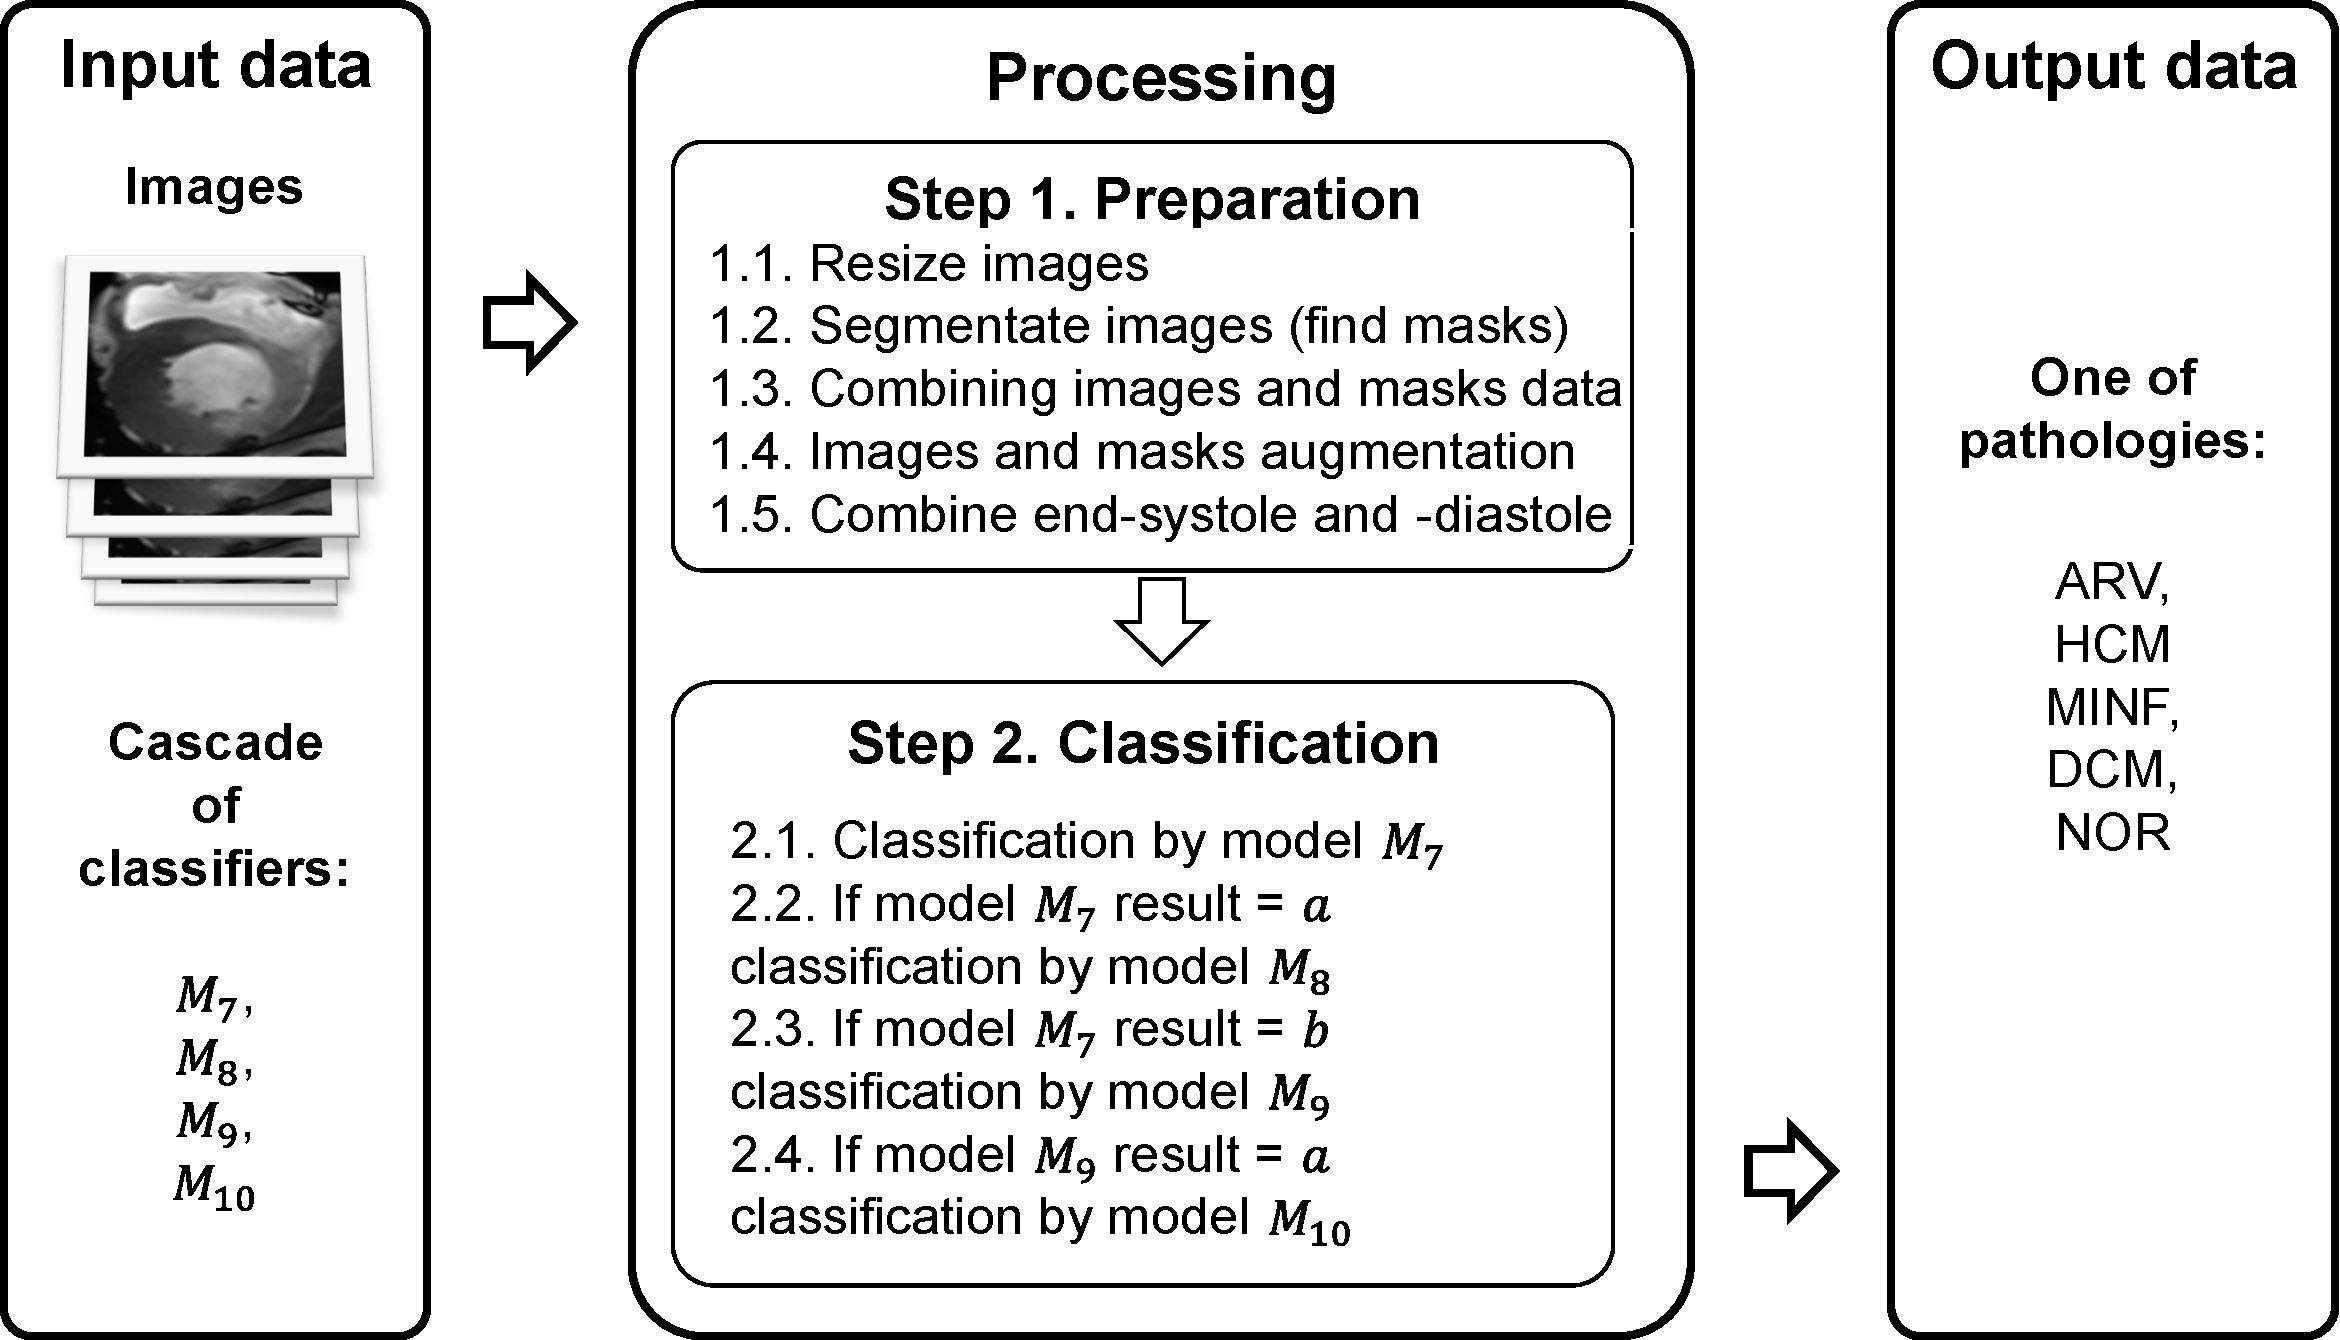
\includegraphics[width=0.8\linewidth]{img/56_fig_7_method-class.pdf}
\caption{Scheme of the pathology classification process using cardiac MRI of an arbitrary patient.}
\label{fig:pathology_classification_process}
\end{figure}

The main steps of the method of cardiac MRIs cascade classification are presented below.

The input data consists of a set of cardiac MRI scans of an arbitrary patient containing images during the diastolic and systolic phases of the cardiac cycle.

\begin{enumerate}[label=Step \arabic*:, leftmargin=5em]
    \item Preparation of MRI scans.
    \begin{enumerate}[label=Step 1.\arabic*:, leftmargin=2.5em]
        \item All MRI scans are cropped to retain only the area with the necessary segments (identified using the first method) and resized to a uniform size.
        \item All patient images are segmented using the multi-stage MRI scan segmentation method.
        \item Image and mask data are combined (each heart segment corresponding to the mask is presented in a separate channel).
        \item Image and mask data are augmented to obtain the number of elements corresponding to the trained model (21 images).
        \item Masks and images from the diastolic and systolic phases of the cardiac cycle are combined.
    \end{enumerate}
    \item Application of the Cascade of Classifiers to Determine Pathologies.
    \begin{enumerate}[label=Step 2.\arabic*:, leftmargin=2.5em]
        \item Application of classifier \({M_7}\).
        \item If the result from \({M_7}\) corresponds to class a, apply classifier \({M_8}\).
        \item If the result from \({M_7}\) corresponds to class b, apply classifier \({M_9}\).
        \item If the result from \({M_9}\) corresponds to class a, apply classifier \({M_{10}}\).
    \end{enumerate}
\end{enumerate}

The output of the method is the determination of one of the following pathologies: ARV, HCM, MINF, DCM, or NOR.

\subsection*{Method of Interpreting Obtained Decisions based on Cardiac MRI}

\subsubsection*{Features Indicating Heart Diseases}

To elucidate the decisions made by DL models, it is essential to transform DL architecture outputs into clinically relevant features used by physicians for diagnosing heart diseases. The following key feature groups are formulated based on the heart diseases addressed in this study.

\begin{enumerate}[label=Group \arabic*:, leftmargin=6em]
    \item Ventricular volumes. Heart volume indicators assess the function of the LV and RV). The ratio of LV volume to RV volume at the ES evaluates ventricular balance during contraction. LV volumes at ES and ED indicate contractile ability and blood capacity, respectively. Similarly, RV volumes help identify dysfunctions; for instance, increased RV volume at the ED may signify ARV, while decreased LV volume at the ES may suggest HCM as investigated in \cite{Izquierdo:2021,Afshin:2014}.
    \item Ejection fraction. Ejection fraction measures the efficiency of blood ejection by the ventricles. LV ejection fraction reflects the proportion of blood pumped out during each contraction, which is crucial for diagnosing DCM, where it is typically reduced. RV ejection fraction indicates the pumping efficiency of the RV, which is crucial for diagnosing ARV \cite{Afshin:2014}.
    \item Volume-to-mass ratios. This group assesses the ratio of heart volumes to myocardial mass, aiding in detecting pathological changes. An increased myocardial mass relative to LV volume may indicate hypertrophic changes, while a decreased ratio suggests dilative processes as stated in \cite{Zheng:2019,Afshin:2014}.
    \item Thickness and variability of the myocardium walls. Myocardial wall thickness and its variability are vital for classifying heart diseases. Increased wall thickness during diastole may indicate HCM, whereas decreased thickness suggests dilative processes. Variability in wall thickness during the cardiac cycle assesses the uniformity of myocardial contractions, with high variability pointing to uneven contractions characteristic of specific cardiomyopathies like HCM, following \cite{Izquierdo:2021}.
\end{enumerate}

\subsubsection*{Interpretation and Visualization Model}

Below is the information model for interpreting decisions made by deep learning models using transformations \({F_d}\):
\begin{equation}
    {F_d}:I \to {O_d},
\end{equation}

where d indicates the pathology (1 – DCM, 2 – HCM, 3 – MINF, 4 – ARV, 5 – NOR), I is the segmented MRI scan, and \({O_d}\) is a set of features for pathology d defined as follows:
\begin{equation}
    {O_d} = \{ o_1^d, \ldots ,o_{{N_d}}^d\} ,\quad {\kern 1pt} o_i^d = ({\rm{name}},{\rm{typ}}{{\rm{e}}_j}),
\end{equation}

with ‘name’ as the feature name and ‘\({\rm{typ}}{{\rm{e}}_j}\)’ as the presentation mode: \({\rm{typ}}{{\rm{e}}_1}\) – 17-segment myocardium model, \({\rm{typ}}{{\rm{e}}_2}\) – circular chart, and \({\rm{typ}}{{\rm{e}}_3}\) – numeric representation.

Below are the measures for each pathology from the set per equation (10), along with recommended visualization methods.

\begin{itemize}
    \item d = 1 – DCM: \(o_1^1\) = (LV ED volume, \({\rm{typ}}{{\rm{e}}_3}\)); \(o_2^1\) = (LV ES volume, \({\rm{typ}}{{\rm{e}}_3}\)); \(o_3^1\) = (LV ejection fraction, \({\rm{typ}}{{\rm{e}}_3}\)); \(o_4^1\) = (myocardial mass at ED, \({\rm{typ}}{{\rm{e}}_3}\)); \(o_5^1\) = (ratio of myocardial mass to LV ED volume, \({\rm{typ}}{{\rm{e}}_2}\)); \(o_6^1\) = (maximum average myocardial wall thickness in ED, \({\rm{typ}}{{\rm{e}}_1}\)).
    \item d = 2 – HCM: \(o_1^2\) = (LV ES volume, \({\rm{typ}}{{\rm{e}}_3}\)); \(o_2^2\) = (LV ejection fraction, \({\rm{typ}}{{\rm{e}}_3}\)); \(o_3^2\) = (ratio of myocardial mass to LV ES volume, \({\rm{typ}}{{\rm{e}}_2}\)); \(o_4^2\) = (maximum average myocardial wall thickness in ED, \({\rm{typ}}{{\rm{e}}_1}\)); \(o_5^2\) = (mean standard deviation of wall thickness in ES, \({\rm{typ}}{{\rm{e}}_3}\)); \(o_6^2\) = (mean standard deviation of wall thickness in ED, \({\rm{typ}}{{\rm{e}}_3}\)).
    \item d = 3 – MINF: \(o_1^3\) = (LV ED volume, \({\rm{typ}}{{\rm{e}}_3}\)); \(o_2^3\) = (LV ejection fraction, \({\rm{typ}}{{\rm{e}}_3}\)); \(o_3^3\) = (myocardial mass at ED, \({\rm{typ}}{{\rm{e}}_3}\)); \(o_4^3\) = (maximum average myocardial wall thickness in ED, \({\rm{typ}}{{\rm{e}}_1}\)); \(o_5^3\) = (mean standard deviation of wall thickness in ED, \({\rm{typ}}{{\rm{e}}_3}\)).
    \item d = 4 – ARV: \(o_1^4\) = (RV ED volume, \({\rm{typ}}{{\rm{e}}_3}\)); \(o_2^4\) = (RV ejection fraction, \({\rm{typ}}{{\rm{e}}_3}\)); \(o_3^4\) = (ratio of LV to RV ED volumes, \({\rm{typ}}{{\rm{e}}_2}\)); \(o_4^4\) = (maximum average myocardial wall thickness in ES, \({\rm{typ}}{{\rm{e}}_1}\)); \(o_5^4\) = (mean standard deviation of wall thickness in ES, \({\rm{typ}}{{\rm{e}}_3}).\)
    \item d = 5 – NOR: \(o_1^5\) = (LV ES volume, \({\rm{typ}}{{\rm{e}}_3}\)); \(o_2^5\) = (LV ED volume, \({\rm{typ}}{{\rm{e}}_3}\)); \(o_3^5\) = (ratio of LV to RV ED volumes, \({\rm{typ}}{{\rm{e}}_2}\)); \(o_4^5\) = (LV ejection fraction, \({\rm{typ}}{{\rm{e}}_3}\)); \(o_5^5\) = (maximum average myocardial wall thickness in ES, \({\rm{typ}}{{\rm{e}}_1}\)).
\end{itemize}

Hence, volumes and ejection fraction are displayed numerically, ratios with circular charts, and wall thickness/variability using the 17-segment model. This layout helps clinicians grasp key cardiac metrics from a single image without comparing multiple MRI slices.

\subsubsection*{Main Steps of the Proposed Method}

This section outlines the main steps of the method for interpreting results obtained through DL means. The primary goal of the method is to present key features in a format suitable for visualization and analysis, thereby ensuring transparency in the pathology classification process. The overall scheme of the result interpretation method is depicted in Figure \ref{fig:interpretation_method_scheme}. The steps, input, and output information are described below.

\begin{figure}[ht]
\centering
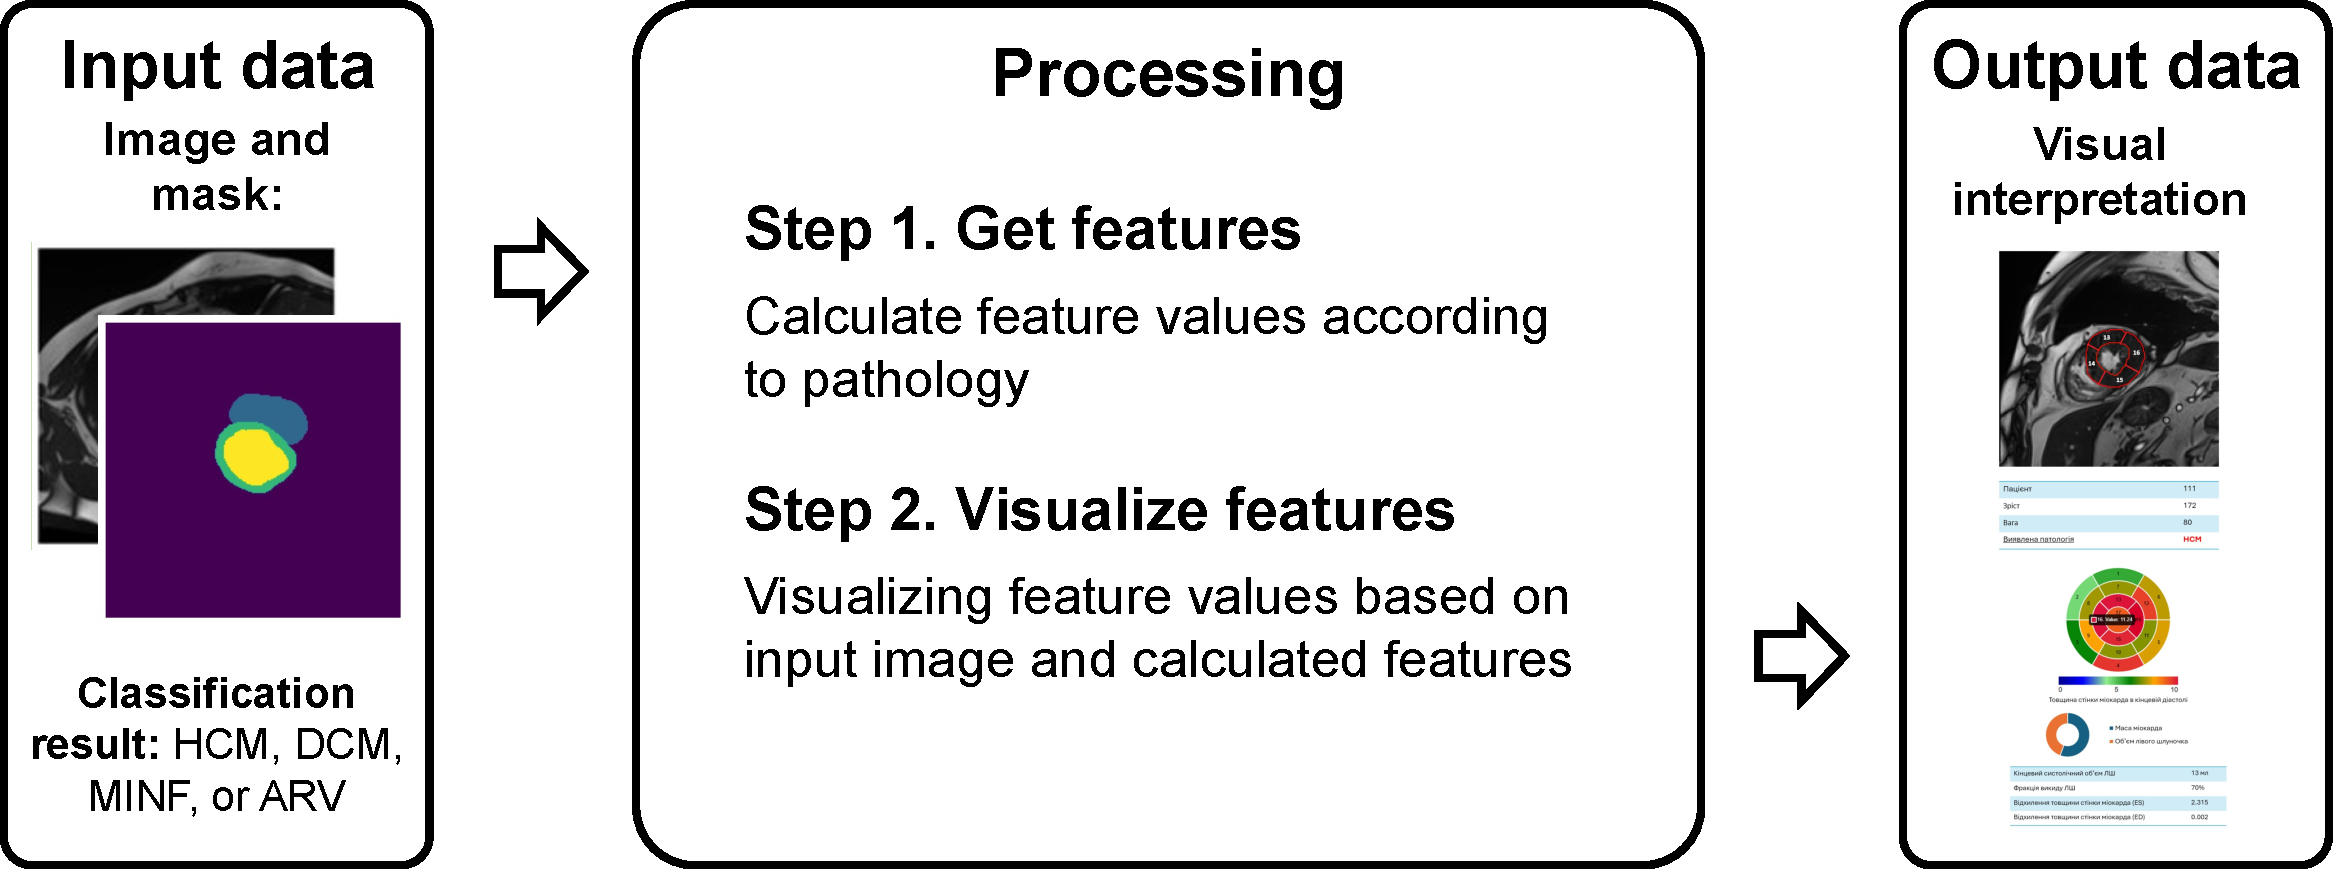
\includegraphics[width=0.8\linewidth]{img/56_fig_8_method-interpret.pdf}
\caption{The overall scheme of the proposed interpretation method.}
\label{fig:interpretation_method_scheme}
\end{figure}

The input data for the method consists of a segmented MRI scan (using the multi-stage segmentation method) and its classification result.

\begin{enumerate}[label=Step \arabic*:, leftmargin=5em]
    \item Obtaining feature values. The values of features for pathology d are determined from the input image. This provides a numerical basis for further analysis.
    \item Presentation of obtained features. The features are presented to the end user separately by types for the corresponding pathologies.
\end{enumerate}

The output of the method is the input segmented and classified MRI scan along with the visualized type features.

Thus, the main steps of the decision interpretation method enhance the accessibility and comprehensibility of the obtained data for further analysis. Users, including physicians and researchers, can assess the classification results by calculating key features and visualizing them. This increases trust in the DL models and facilitates their practical use in diagnosing patients with heart pathologies.

\subsection*{Evaluation Approaches and Metrics}

In this study, we utilized several essential metrics to assess the performance of our DL models in medical applications, covering both segmentation and multiclass classification tasks. Our findings are consistent with existing research on model evaluation in medical image analysis, as highlighted in Rainio et al. \cite{Rainio:2024}.

\subsubsection*{Experimental Models for Validating the Multi-Stage Segmentation Method}

To objectively measure how each stage of the multi-stage segmentation method affects final segmentation quality, a series of experiments was performed with identical epochs, architectures, and data. Results were averaged over 10 training/testing cycles, and segmentation accuracy was assessed using the Dice coefficient, comparing predicted and expert masks.

To evaluate the combined impact of these steps, an arithmetic mean of Dice across all structures (LV, RV and myocardium) in both ES and ED phases was calculated. Six additional models were developed to test specific components:

\begin{itemize}
    \item Base model \(M_1^{\exp 1}\): Trained without any optional preprocessing or postprocessing (only uniform resizing). It serves as a baseline for recognizing heart structures on the original ACDC dataset.
    \item Localization models \(M_1^{\exp 2}\) and \(M_2^{\exp 2}\): \(M_1^{\exp 2}\) localizes the heart region as a single binary mask, while \(M_2^{\exp 2}\) segments LV, RV, and myocardium within that localized region. Both share the same input ACDC dataset.
    \item Decomposition models \(M_1^{\exp 3}\), \(M_2^{\exp 3}\) and \(M_3^{\exp 3}\): Each model handles binary segmentation of one structure (LV, RV, or myocardium) using decomposed masks. The same ACDC dataset is resized and split accordingly.
\end{itemize}

These experiments compare partial versus combined stages, verifying each stage’s effectiveness and its contributions to overall segmentation accuracy.

\subsubsection*{Metrics for Evaluating the Cascade Classification Method Results}

To measure classification performance, each classifier’s accuracy is computed at every step, then averaged. Equations for calculating class-specific and overall accuracies—namely for NOR, ARV, HCM, MINF, and DCM—are formalized as follows:
\begin{equation}
    {A_{{\rm{NOR}}{\rm{,ARV}}}} = \frac{{{A_{{\rm{Classifier 1}}}} + {A_{{\rm{Classifier 2}}}}}}{2},
\end{equation}

\begin{equation}
    {A_{{\rm{HCM}}}} = \frac{{{A_{{\rm{Classifier 1}}}} + {A_{{\rm{Classifier 3}}}}}}{2},
\end{equation}

\begin{equation}
    {A_{{\rm{MINF}}{\rm{,DCM}}}} = \frac{{{A_{{\rm{Classifier 1}}}} + {A_{{\rm{Classifier 3}}}} + {A_{{\rm{Classifier 4}}}}}}{3},
\end{equation}

\begin{equation}
    {A_{{\rm{gen}}}} = \frac{{{A_{{\rm{NOR}}}} + {A_{{\rm{ARV}}}} + {A_{{\rm{HCM}}}} + {A_{{\rm{MINF}}}} + {A_{{\rm{DCM}}}}}}{5},
\end{equation}

where \({A_{{\rm{Classifier 1 - 4}}}}\) are the accuracies of each classifier, \({A_{{\rm{NOR}}{\rm{, ARV}}{\rm{, HCM}}{\rm{, MINF}}{\rm{, DCM}}}}\) are the classification accuracies for each individual class, and \({A_{{\rm{gen}}}}\) is the overall accuracy.

Evaluation equations (11)–(14) ensure a fair comparison with existing methods.

Furthermore, standard classification metrics include Accuracy, Precision, Recall, \({F_1}\)-score, and Area Under the Curve (AUC) with Receiver Operating Characteristic (ROC) curves. They are based on counts of true positives, false positives, false negatives, and true negatives. Taken together, these metrics offer a detailed perspective on how effectively the method distinguishes different cardiac pathologies.

\Rone{\revtag{1}{5}\subsubsection*{Evaluation, Uncertainty, and Calibration}}
\Rone{\revtag{1}{5} % Action 6
Segmentation metrics include the Dice coefficient per structure and cardiac phase, reported with 95\% bootstrap confidence intervals (2,000 resamples) to quantify uncertainty. The classification cascade reports Area Under the Receiver Operating Characteristic Curve (AUROC) and Area Under the Precision-Recall Curve (AUPRC), also with 95\% CIs. Model calibration is assessed using reliability diagrams, accompanied by the Expected Calibration Error (ECE) and Maximum Calibration Error (MCE) \cite{Guo:2017}. Operating thresholds for the binary classifiers are determined on the validation folds using Youden’s J-index \cite{Youden:1950}, and we report the corresponding sensitivity and specificity at these thresholds. Paired comparisons to baseline models (e.g., a standard ResNet-50 multiclass classifier) are performed using Wilcoxon signed-rank tests across patients, with false-discovery-rate control for multiple comparisons.
}

\subsubsection*{Evaluation of the Interpretation Method Results}

It should be noted that the quality and accuracy of the results obtained through the proposed approach depend on the metrics of the multi-stage segmentation and cascade classification methods. The interpretation method is designed solely to interpret the decisions made by the previous methods. The method provides feature values derived from MRI scans, which allow the physician to understand why the DL models made specific decisions. It is important to note that this decision is advisory for a physician, who makes the final diagnosis based on the numerical features provided.

The feature values used by the physician to make decisions are obtained in an understandable manner (typically geometric characteristics of different image segments) and do not require additional evaluation using specialized metrics.

\subsection*{Dataset}

This study utilizes the ACDC dataset \cite{Bernard:2018}. It comprises 150 patients and is divided into five groups: 30 healthy patients, 30 patients with a history of myocardial infarction, 30 patients with DCM, 30 patients with HCM, and 30 patients with ARV. For each patient, the data includes physical parameters, a set of images, and expert-annotated masks (ground truth labels) at different stages of the cardiac cycle. The expert masks contain segmented regions for LV, RV, and myocardium. An example element of the \({D_1}\) dataset is illustrated in Figure \ref{fig:dataset_d1_example}.

\Rtwo{\revtag{2}{3} % Action 3 - M&Ms dataset intro
For external validation, we utilized the Multi-Centre, Multi-Vendor and Multi-Disease Cardiac Segmentation (M\&Ms) challenge dataset \cite{Campello:2021}. This dataset contains 375 CMR studies from six hospitals, acquired using four different scanner vendors (Siemens, Philips, General Electric, Canon). The performance of our models, trained exclusively on ACDC data, was evaluated on the M\&Ms test set to assess their generalizability under significant domain shift.
}

\begin{figure}[ht]
\centering
\begin{tabular}{cc}
    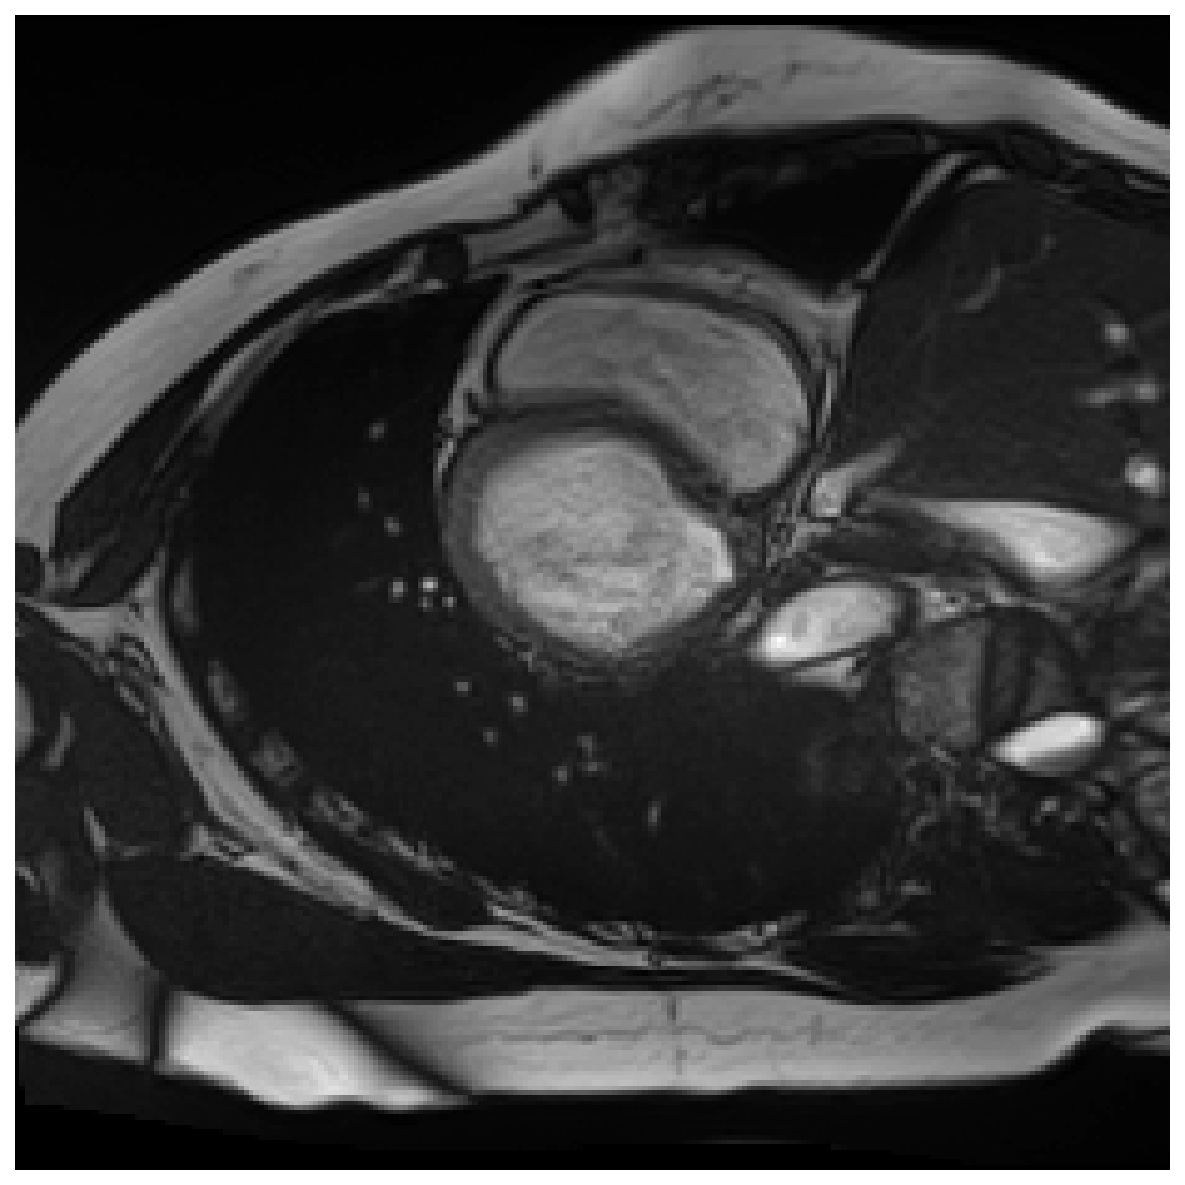
\includegraphics[width=0.3\linewidth]{img/56_fig_9a.pdf} &
    
\includegraphics[width=0.3\linewidth]{img/56_fig_9b.pdf} \\
    \textbf{\textsf{(a)}} & \textbf{\textsf{(b)}}
\end{tabular}
\caption{Example from the dataset \({D_1}\) with a cardiac MRI scan \textbf{(a)} and its mask \textbf{(b)}.}
\label{fig:dataset_d1_example}
\end{figure}

For training and testing the models (\({M_1}\)–\({M_{10}}\)), corresponding dataset modifications were created. Below, we examine examples of dataset elements and their characteristics.

For training the localization models (\({M_1}\)–\({M_3}\)), dataset \({D_2}\) was created, containing 2,978 MRI scans. All images were cropped to retain only the necessary segments (identified using the first method) and resized to a uniform resolution (256 × 256 pixels) with an aspect ratio of 1:1. For each image, separate masks were generated for each of the studied heart structures (LV, RV, and myocardium). An example element of dataset \({D_2}\) is shown in Figure \ref{fig:dataset_d2_example}.

\begin{figure}[ht]
\centering
\begin{tabular}{cccc}
    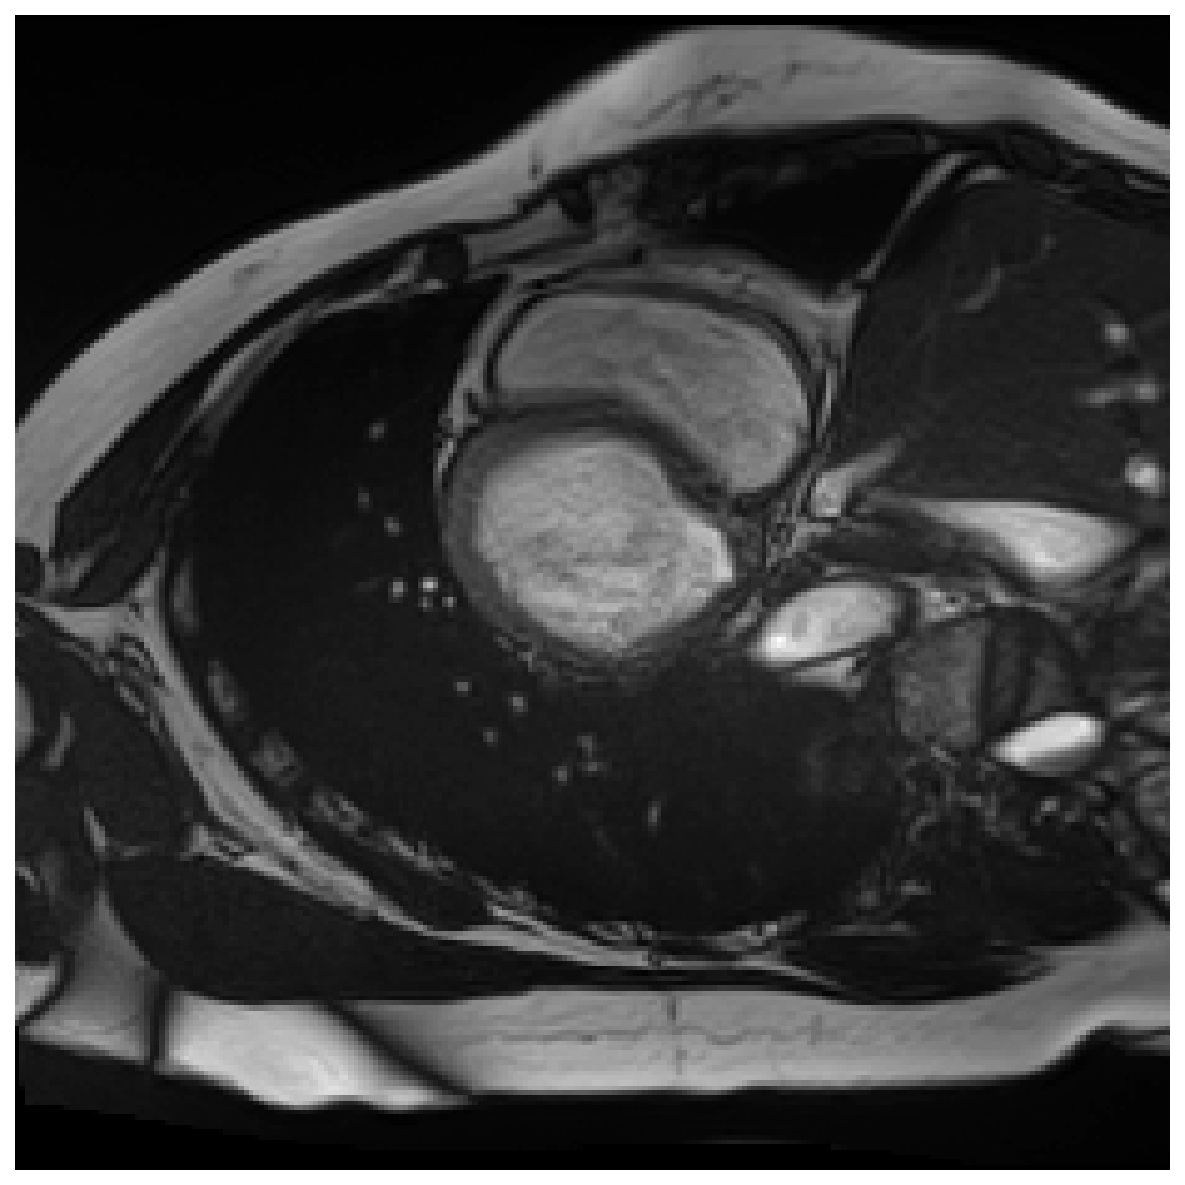
\includegraphics[width=0.22\linewidth]{img/56_fig_10a.pdf} &
    
\includegraphics[width=0.22\linewidth]{img/56_fig_10b.pdf} &
    
\includegraphics[width=0.22\linewidth]{img/56_fig_10c.pdf} &
    
\includegraphics[width=0.22\linewidth]{img/56_fig_10d.pdf} \\
    \textbf{\textsf{(a)}} & \textbf{\textsf{(b)}} & \textbf{\textsf{(c)}} & \textbf{\textsf{(d)}}
\end{tabular}
\caption{Instance element of dataset \({D_2}\): \textbf{(a)} MRI scan, \textbf{(b)} myocardium segment mask, \textbf{(c)} LV segment mask, and \textbf{(d)} RV segment mask.}
\label{fig:dataset_d2_example}
\end{figure}

For training the mask generation models (\({M_4}\)–\({M_6}\)), corresponding datasets \({D_3}\), \({D_4}\), and \({D_5}\) were created. These datasets, based on \({D_2}\), contain the same number of images. All images in these datasets have a uniform resolution (64 × 64) and an aspect ratio of 1:1. Each dataset corresponds to a specific heart structure:

\begin{itemize}
    \item Dataset \({D_3}\): contains localized images of the LV and the corresponding localized mask. An example element of dataset \({D_3}\) is shown in Figure \ref{fig:dataset_d345_example}a-b.
    \item Dataset \({D_4}\): contains localized images of the RV and the corresponding localized mask. An example element of dataset \({D_4}\) is shown in Figure \ref{fig:dataset_d345_example}c-d.
    \item Dataset \({D_5}\): contains localized images of the myocardium and the corresponding localized mask. An example element of dataset \({D_5}\) is shown in Figure \ref{fig:dataset_d345_example}e-f.
\end{itemize}

\begin{figure}[ht]
\centering
\begin{tabular}{cccccc}
    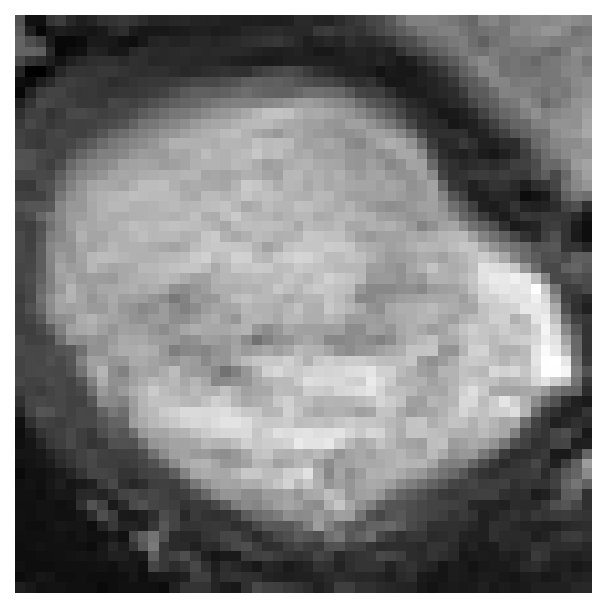
\includegraphics[width=0.14\linewidth]{img/56_fig_11a.pdf} &
    
\includegraphics[width=0.14\linewidth]{img/56_fig_11b.pdf} &
    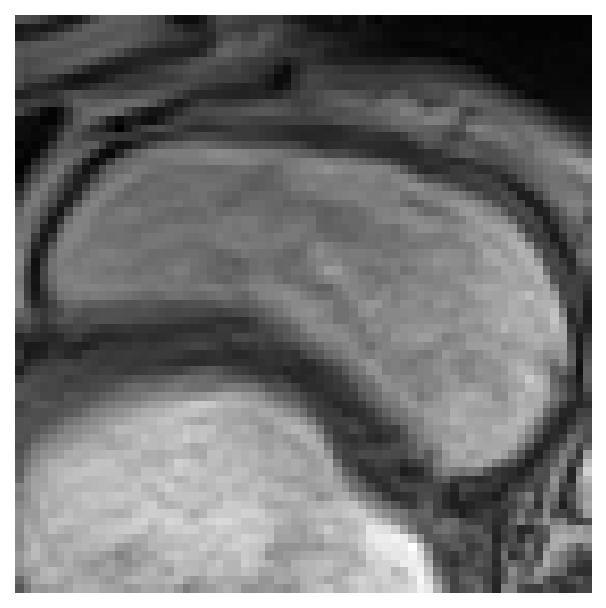
\includegraphics[width=0.14\linewidth]{img/56_fig_11c.pdf} &
    
\includegraphics[width=0.14\linewidth]{img/56_fig_11d.pdf} &
    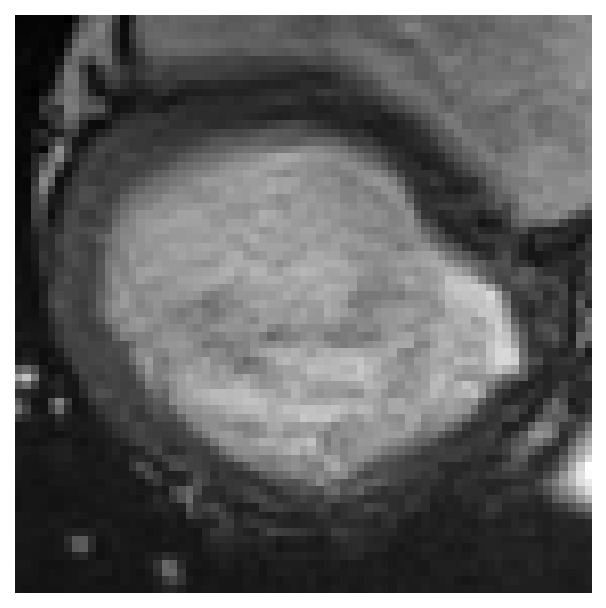
\includegraphics[width=0.14\linewidth]{img/56_fig_11e.pdf} &
    
\includegraphics[width=0.14\linewidth]{img/56_fig_11f.pdf} \\
    \textbf{\textsf{(a)}} & \textbf{\textsf{(b)}} & \textbf{\textsf{(c)}} & \textbf{\textsf{(d)}} & \textbf{\textsf{(e)}} & \textbf{\textsf{(f)}}
\end{tabular}
\caption{Example elements of created datasets: \({D_3}\) – \textbf{(a)} MRI scan, \textbf{(b)} LV segment mask; \({D_4}\) – \textbf{(c)} MRI scan, \textbf{(d)} RV segment mask; \({D_5}\) – \textbf{(e)} MRI scan, \textbf{(f)} myocardium segment mask.}
\label{fig:dataset_d345_example}
\end{figure}

For training the cascade classification models (\({M_7}\)–\({M_{10}}\)), dataset \({D_6}\) was formed. This dataset contains modified MRI scans for each patient and their corresponding pathology classes. The modification involves placing each heart segment (LV, RV, and myocardium) in separate channels of the RGB color model. All images were cropped according to the largest localization area from a single patient’s dataset and have a uniform resolution (64 × 64) with an aspect ratio of 1:1. The entire dataset includes, like the original dataset, 150 patients divided into five groups. An example element of dataset \({D_6}\) is shown in Figure \ref{fig:dataset_d6_example}.

\begin{figure}[ht]
\centering
\begin{tabular}{c}
    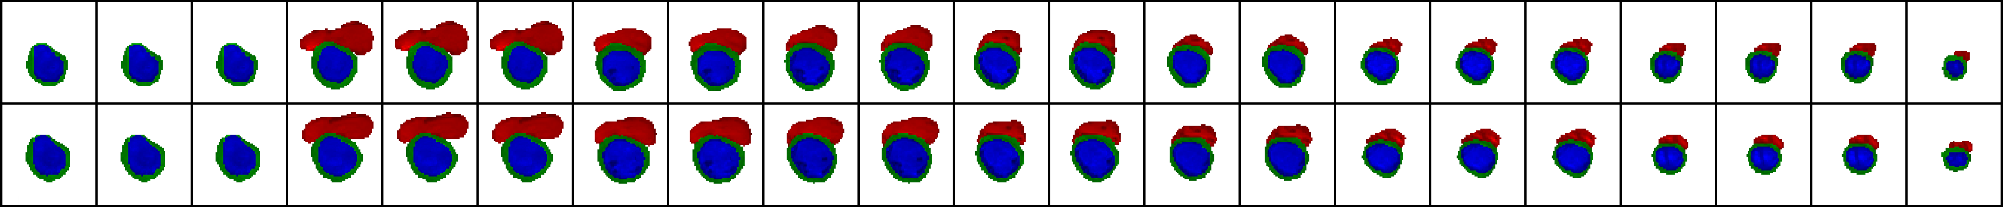
\includegraphics[width=1.0\linewidth]{img/56_fig_12a.pdf} \\
    \textbf{\textsf{(a)}} \\
    
\includegraphics[width=0.1\linewidth]{img/56_fig_12b.pdf} \\
    \textbf{\textsf{(b)}}
\end{tabular}
\caption{Example element of dataset \({D_6}\): \textbf{(a)} set of modified MRI scans and \textbf{(b)} pathology class label (MINF).}
\label{fig:dataset_d6_example}
\end{figure}

Thus, five new datasets \({D_2}\)–\({D_6}\) were created, which are used for localizing regions of interest, determining precise contours in MRI scans, and classifying MRI scans into pathology classes.

\section*{Results and Discussion}

\subsection*{Results of the Segmentation Method}

To validate the proposed multi-stage segmentation method, a comparison of results with those from other studies was conducted, specifically comparing the segmentation accuracy of individual heart structures using the Dice coefficient. Additionally, to confirm the positive impact of the proposed method steps on the final segmentation quality, a series of experiments were performed, progressively increasing the complexity of the model training by adding individual steps or their combinations while calculating segmentation accuracy metrics. The following experiments were conducted:

\begin{enumerate}
    \item Segmentation of original MRI scans: To determine the baseline capability of the DL model to recognize heart structures.
    \item Segmentation of localized MRI scans using original masks: To evaluate the impact of preliminary localization on the final segmentation result.
    \item Segmentation of original images using decomposed masks: To assess the use of binary segmentation instead of multi-structure segmentation.
    \item Segmentation of localized MRI scans using decomposed masks: To evaluate the combination of preliminary localization and binary segmentation instead of multi-structure segmentation.
    \item Segmentation of localized MRI scans using decomposed masks with postprocessing (proposed approach): To assess the combination of all steps of the proposed method.
\end{enumerate}

These experiments aim to determine each step’s contribution to improving segmentation accuracy, particularly in complex areas such as myocardium and RV.
To objectively measure the contribution of each component of our proposed method, we conducted a detailed ablation study. The results, summarized in Table \ref{tab:experiments_comparison}, demonstrate the incremental improvements gained from localization, mask decomposition, and post-processing steps.

The authors of the ACDC dataset \cite{Bernard:2018} separately formed training and testing datasets consisting of 100 and 50 patients, respectively. Using pre-formed datasets instead of custom splits allows for more accurate comparisons of experimental results with those from other studies by utilizing the same test dataset. Therefore, all experiments in this section use the pre-formed test dataset provided by the authors.

\subsubsection*{Segmentation of Localized MRI Scans using Decomposed Masks with Postprocessing (Proposed Approach)}

In the fifth and final stage of the experiments, all previous stages were applied, thereby implementing the complete scheme of the proposed method, which combines localization, decomposition of masks, and postprocessing of mask contours.

Localization and mask generation were conducted similarly to the previous experiment, utilizing models (\({M_1}\)–\({M_6}\)). Unlike previous experiments, after obtaining segmentation results, postprocessing was performed to enhance the quality of the segmented masks. This stage included contour smoothing to eliminate artifacts that might have arisen from minor mislabeling or noise in the data. Postprocessing also involved applying blurring methods to reduce sharp transitions between different regions and create a more natural appearance of the segmented structure contours. Additionally, masks were resized back to their original dimensions to ensure accurate comparison with expert masks.

Applying postprocessing allowed residual artifacts that could degrade segmentation quality, especially for the RV where weak contrast and overlap with adjacent tissues are common, to be removed. Masks obtained after this stage demonstrated higher conformity to expert masks.
The results obtained for the final stage of the experiments are shown separately for ED and ES in Table \ref{tab:experiment_5_results}.

\begin{table}[ht]
\centering
\caption{Results of the fifth experiment. This table contains the obtained mean Dice values for different segments. Numbers in \textbf{bold} show the highest scores.}
\label{tab:experiment_5_results}
\begin{tabular}{lcccccc}
\toprule
\textbf{Models} & \multicolumn{3}{c}{\textbf{ED}} & \multicolumn{3}{c}{\textbf{ES}} \\
\cmidrule(lr){2-4} \cmidrule(lr){5-7}
 & \textbf{LV} & \textbf{RV} & \textbf{Myocardium} & \textbf{LV} & \textbf{RV} & \textbf{Myocardium} \\
\midrule
\(M_1^{{{\exp }_1}}\) & 0.911 & 0.842 & 0.812 & 0.890 & 0.871 & 0.832 \\
\begin{tabular}[c]{@{}l@{}}\({M_1}\), \({M_2}\), \({M_3}\),\\\({M_4}\), \({M_5}\), \({M_6}\)\\+ postprocessing\end{tabular} & \textbf{0.974} & \textbf{0.947} & \textbf{0.896} & \textbf{0.940} & \textbf{0.915} & \textbf{0.920} \\
\bottomrule
\end{tabular}
\end{table}

The proposed approach achieved the best results among all experimental stages, providing maximum segmentation accuracy for all studied structures, particularly the LV and myocardium, which are crucial for medical analysis. Therefore, the combination of localization, decomposition, and postprocessing confirmed its effectiveness as a comprehensive strategy for automated segmentation of heart structures in MRI scans. The comparison of all experimental results for evaluating the effectiveness of the localization, decomposition, and postprocessing steps is presented in Table \ref{tab:experiments_comparison}.

\begin{table}[ht]
\centering
\caption{Computational results, i.e., Dice coefficient values, for evaluating the effectiveness of localization, decomposition, and postprocessing steps in the proposed segmentation method. Numbers in \textbf{bold} show the highest scores.}
\label{tab:experiments_comparison}
\begin{tabular}{lcccccc}
\toprule
\textbf{Experiments} & \multicolumn{3}{c}{\textbf{ED}} & \multicolumn{3}{c}{\textbf{ES}} \\
\cmidrule(lr){2-4} \cmidrule(lr){5-7}
 & \textbf{LV} & \textbf{RV} & \textbf{Myocardium} & \textbf{LV} & \textbf{RV} & \textbf{Myocardium} \\
\midrule
Experiment 1 & 0.911 & 0.842 & 0.812 & 0.890 & 0.871 & 0.832 \\
Experiment 2 & 0.920 & 0.902 & 0.875 & 0.894 & 0.891 & 0.884 \\
Experiment 3 & 0.919 & 0.892 & 0.855 & 0.887 & 0.873 & 0.885 \\
Experiment 4 & 0.956 & 0.939 & 0.866 & 0.930 & 0.905 & 0.898 \\
\begin{tabular}[c]{@{}l@{}}Experiment 5\\(proposed approach)\end{tabular} & \textbf{0.974} & \textbf{0.947} & \textbf{0.896} & \textbf{0.940} & \textbf{0.915} & \textbf{0.920} \\
\bottomrule
\end{tabular}
\end{table}

A visual comparison of all experimental results is depicted in Figure \ref{fig:experiments_dice_comparison}.

\begin{figure}[ht]
\centering
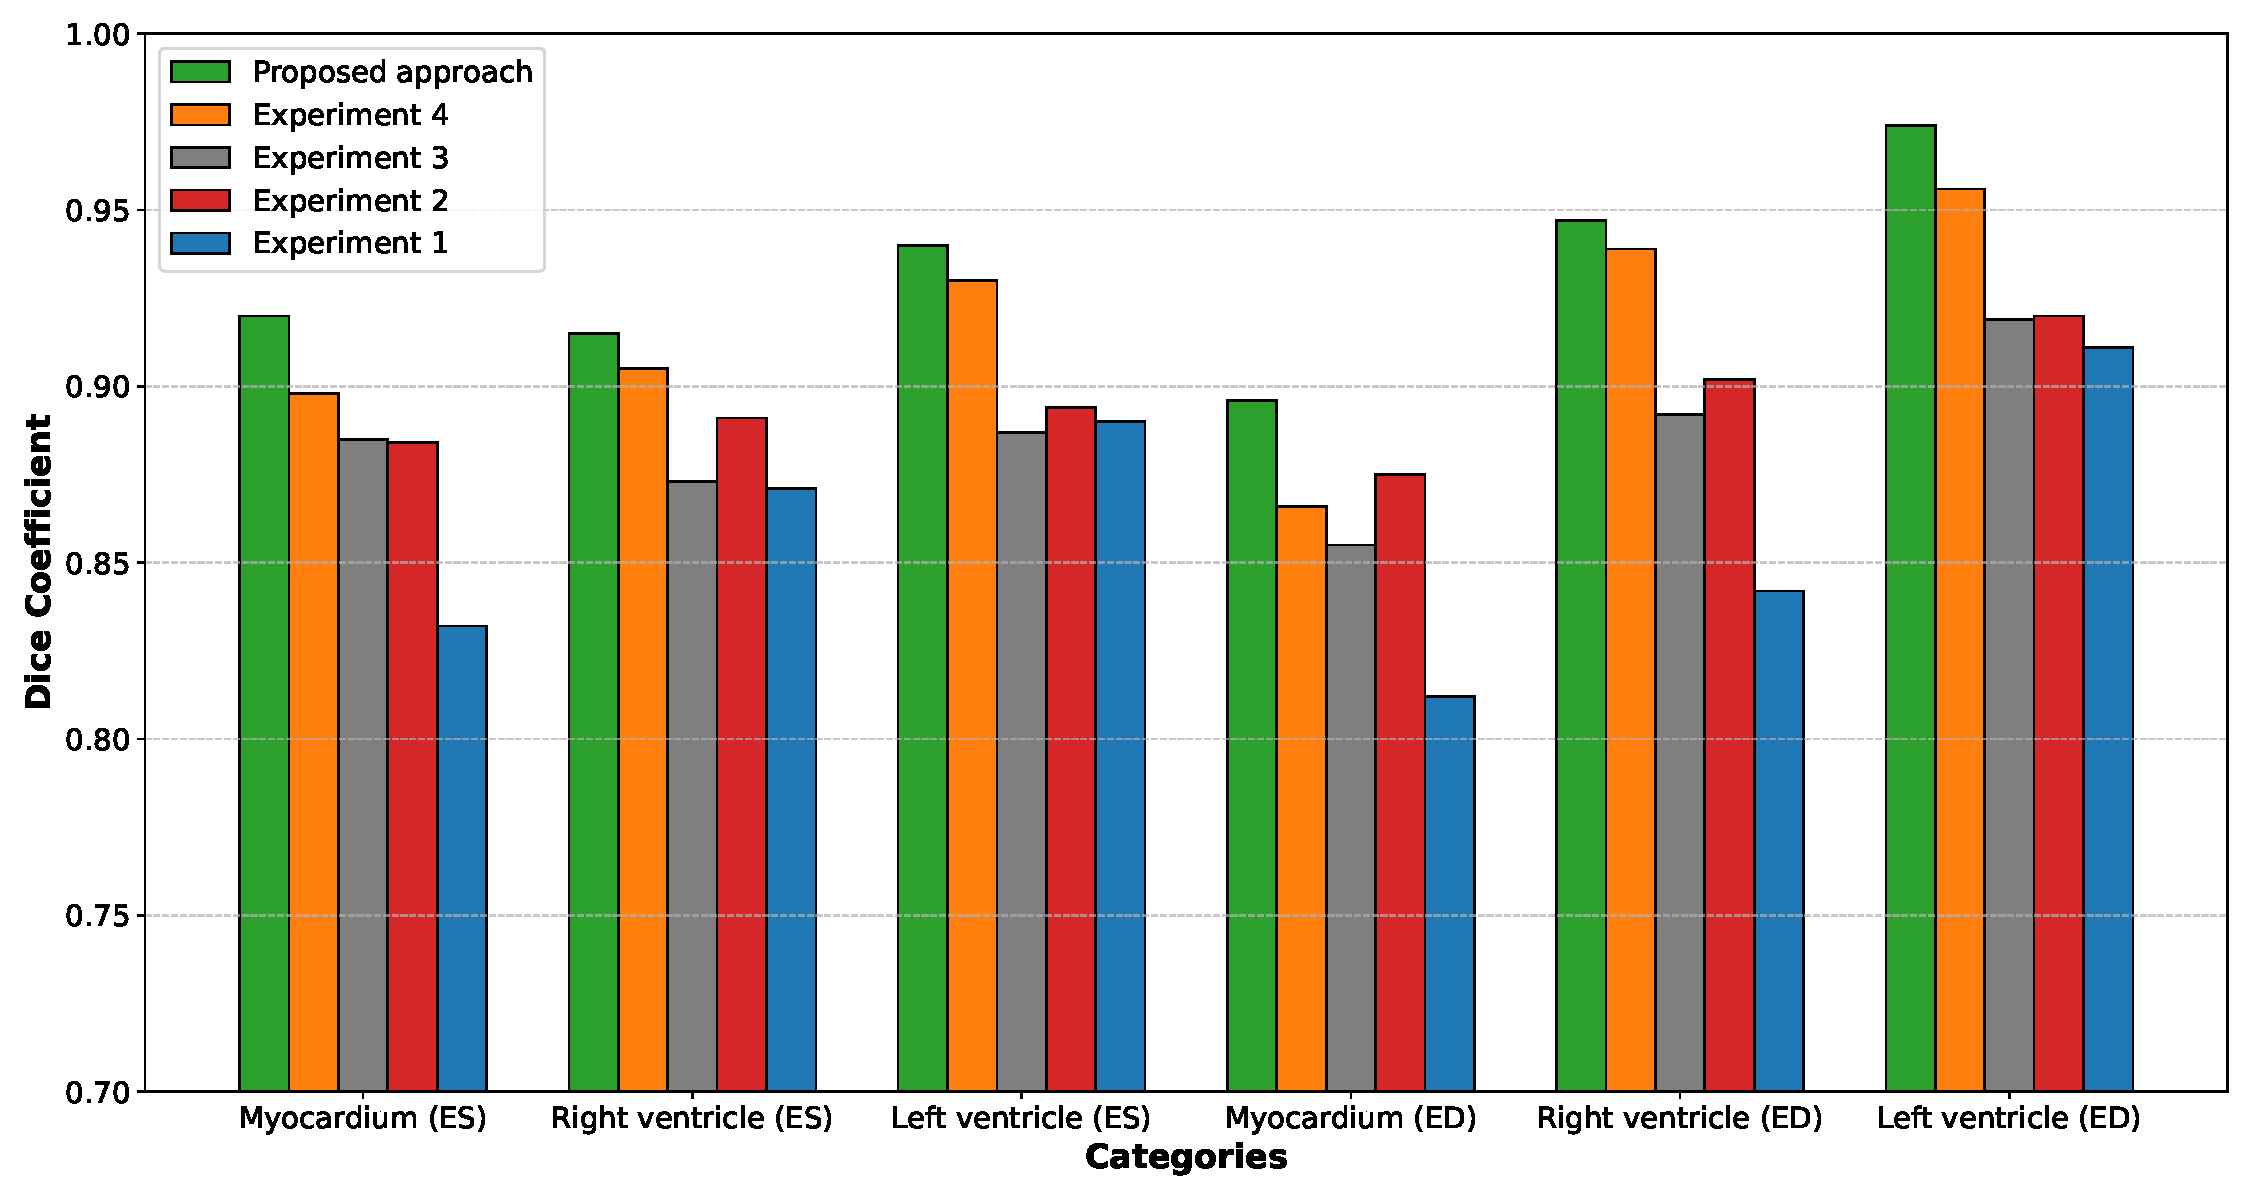
\includegraphics[width=0.8\linewidth]{img/56_fig_13.pdf}
\caption{Visual comparison of obtained Dice coefficient values for experiments 1–5 (ES – end-systole, ED – end-diastole).}
\label{fig:experiments_dice_comparison}
\end{figure}

Thus, the experiments demonstrated an increase in segmentation accuracy using the proposed method, which includes localization, decomposition, and postprocessing of images. The overall segmentation accuracy for all structures according to the average Dice coefficient increased to 0.932, which is 7.76\% higher compared to the base model \(M_1^{{{\exp }_1}}\). Therefore, the proposed approach ensures high segmentation accuracy of heart structures in MRI scans, which is critically important for subsequent clinical analysis and diagnosis.

\subsubsection*{Comparison of the Proposed Approach with Current Segmentation Methods}

The obtained segmentation results were compared with the current methods described in the literature, separately for each structure, using the Dice coefficient for the ED and ES phases.

For the LV, the proposed method achieved the highest Dice coefficient values: 0.974 in the ED phase and 0.940 in the ES phase. Compared to the method by Hu et al. \cite{Hu:2023}, which is the closest competitor, the proposed method shows better results, indicating its ability to provide more accurate contour delineation.

Segmentation of the RV, traditionally considered a challenging task due to weak contrast with adjacent tissues, also demonstrates the advantages of the proposed method. In the ED phase, the Dice coefficient was 0.947, the highest among all compared methods, surpassing the closest results by Hu et al. In the ES phase, accuracy remains the highest among competing approaches.

Regarding the segmentation of the myocardium of the LV, the proposed method showed significant improvement. In the ED phase, the Dice coefficient reached 0.896, which is lower than the closest results by Hu et al. but better than those of other competitors, particularly Bourfiss et al., where this indicator was only 0.875. In the ES phase, the proposed approach achieved the highest value among all compared studies – 0.920, slightly exceeding the closest result by Hu et al.

The indicators of all the aforementioned authors are presented in Table \ref{tab:segmentation_comparison_sota} compared with the proposed method’s results. Our method demonstrates highly competitive performance, particularly for RV segmentation and for all structures in the ES phase. While some methods like Zhang et al. \cite{Zhang:2022} report a slightly higher Dice for LV segmentation in the ED phase (0.976 vs. our 0.974), our approach provides a more balanced and robust performance across all anatomical structures and cardiac phases, which is critical for comprehensive clinical assessment.

\begin{table}[ht]
\centering
\caption{Comparison of segmentation results with the state of the art using by Dice coefficient. Numbers in \textbf{bold} show the highest scores.}
\label{tab:segmentation_comparison_sota}
\begin{tabular}{lcccccc}
\toprule
\textbf{Works} & \multicolumn{3}{c}{\textbf{ED}} & \multicolumn{3}{c}{\textbf{ES}} \\
\cmidrule(lr){2-4} \cmidrule(lr){5-7}
 & \textbf{LV} & \textbf{RV} & \textbf{Myocardium} & \textbf{LV} & \textbf{RV} & \textbf{Myocardium} \\
\midrule
Hu et al. \cite{Hu:2023} & 0.968 & 0.946 & \textbf{0.902} & 0.931 & 0.899 & 0.919 \\
da Silva et al. \cite{daSilva:2024} & 0.963 & 0.932 & 0.892 & 0.911 & 0.883 & 0.901 \\
Ammar et al. \cite{Ammar:2021} & 0.964 & 0.935 & 0.889 & 0.917 & 0.879 & 0.898 \\
Bourfiss et al. \cite{Bourfiss:2023} & 0.959 & 0.929 & 0.875 & 0.921 & 0.885 & 0.895 \\
Hasan \& Linte \cite{Hasan:2020} & 0.963 & 0.924 & 0.901 & 0.929 & 0.887 & 0.913 \\
Zhang et al. \cite{Zhang:2022} & \textbf{0.976} & 0.949 & 0.903 & \textbf{0.950} & 0.916 & 0.918 \\
Ours & 0.974 & \textbf{0.947} & 0.896 & 0.940 & \textbf{0.915} & \textbf{0.920} \\
\bottomrule
\end{tabular}
\end{table}

Thus, the overall segmentation accuracy for all structures according to the average Dice coefficient for the proposed method is 0.932, which is:

\begin{itemize}
    \item 0.54\% higher than the results by Hu et al., who reported an accuracy of 0.927.
    \item 2.08\% higher than the results by da Silva et al., who reported an accuracy of 0.913.
    \item 2.08\% higher than the results by Ammar et al., who reported an accuracy of 0.913.
    \item 2.41\% higher than the results by Bourfiss et al., who reported an accuracy of 0.910.
\end{itemize}

A visual comparison of all experimental results is presented in Figure \ref{fig:sota_dice_comparison}.

\begin{figure}[ht]
\centering
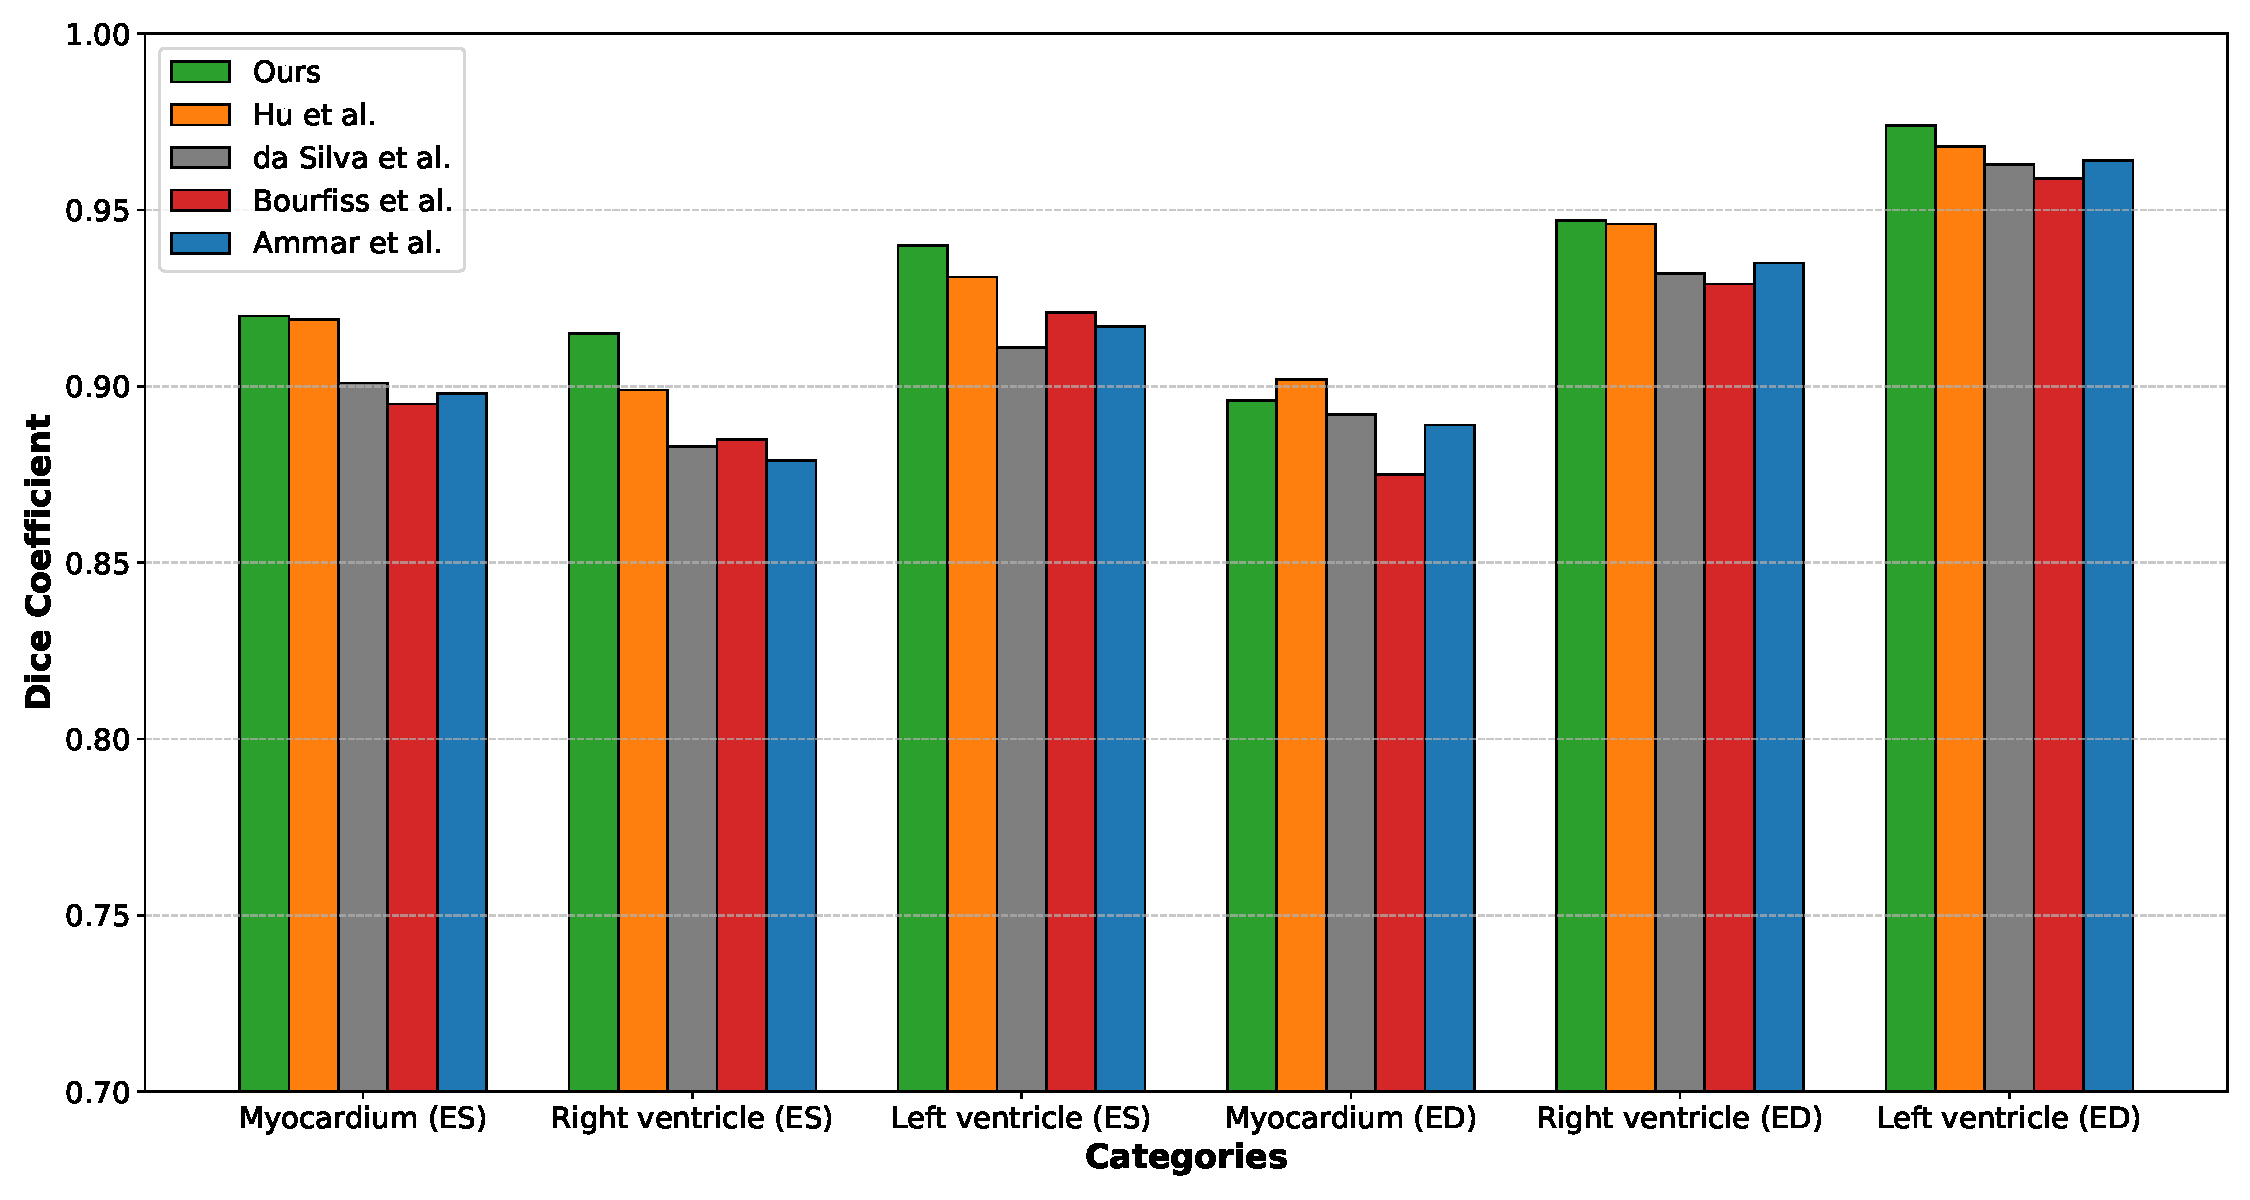
\includegraphics[width=0.8\linewidth]{img/56_fig_14.pdf}
\caption{Visual comparison of obtained Dice coefficient values with the state of the art (ES – end-systole, ED – end-diastole).}
\label{fig:sota_dice_comparison}
\end{figure}

The obtained results indicate that the proposed segmentation method outperforms most current approaches in terms of segmentation accuracy for the LV, RV, and myocardium. Particularly significant improvement is observed in the case of the RV, demonstrating the effectiveness of localization, decomposition, and postprocessing. The method exhibits stability and high accuracy in all phases of the cardiac cycle, making it promising for clinical application.

\subsubsection*{Validation of Expert Masks and Obtained Results by a Medical Specialist}

This study utilized the expert-provided ground truth masks from the ACDC dataset for training and initial validation. However, to rigorously assess the performance of our generated masks, we conducted an additional validation step involving a medical specialist. During the training and testing of the proposed models on the original dataset, certain inaccuracies in the segmentation masks were identified. Even minor discrepancies between training and testing masks can significantly impact the evaluation accuracy. These inaccuracies may involve incorrect labeling of image regions or missing segments. For instance, in Figure \ref{fig:mask_validation_example}, an "extra" area in the upper part of the left ventricle (LV) was erroneously marked by experts as part of the myocardium (Zone 1 in Figure \ref{fig:mask_validation_example}c). In contrast, the proposed method accurately separated this region from the myocardium. Similarly, the model correctly identified a region in the right myocardium that experts had mistakenly excluded (Zone 2 in Figure \ref{fig:mask_validation_example}c).

\begin{figure}[ht]
\centering
\begin{tabular}{ccc}
    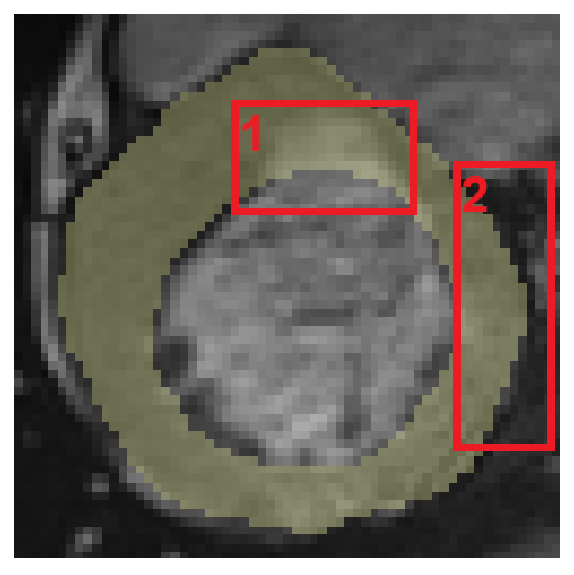
\includegraphics[width=0.25\linewidth]{img/56_fig_15a.pdf} &
    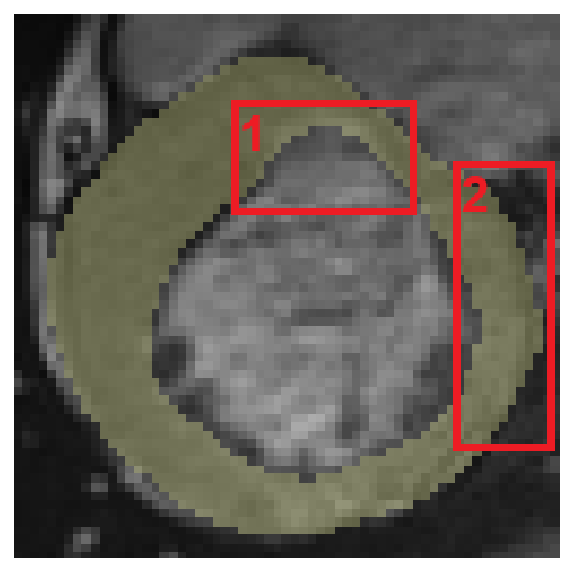
\includegraphics[width=0.25\linewidth]{img/56_fig_15b.pdf} &
    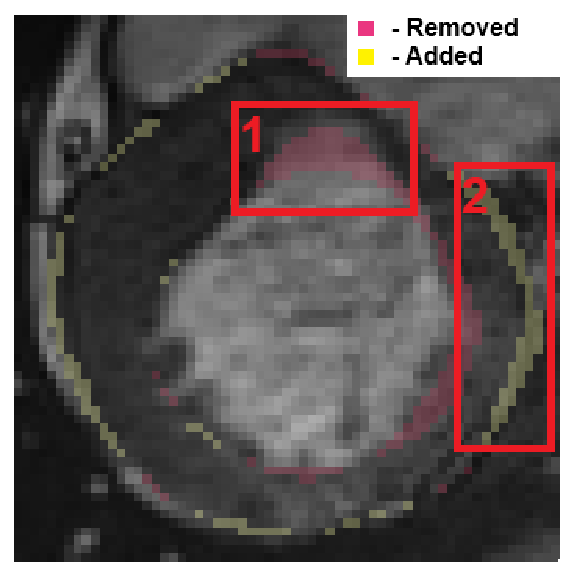
\includegraphics[width=0.25\linewidth]{img/56_fig_15c.pdf} \\
    \textbf{\textsf{(a)}} & \textbf{\textsf{(b)}} & \textbf{\textsf{(c)}}
\end{tabular}
\caption{This figure showcases the impact of insufficient brightness on cardiac MRI analysis. Panel \textbf{(a)} shows the expert mask, \textbf{(b)} the proposed method’s mask, and \textbf{(c)} their differences, where pink marks removed areas and yellow marks added regions. The red rectangles labeled "1" and "2" highlight notable discrepancies in the upper and right parts of the mask.}
\label{fig:mask_validation_example}
\end{figure}

A detailed analysis of masks with less than 95\% overlap between expert and model-generated masks suggested that some discrepancies arose not from model errors but because the DL model provided more precise segmentations differing from expert annotations. To address this, a medical specialist was engaged to validate both the training and testing datasets alongside all the results obtained.

To ensure a comprehensive quality assessment, a unique mask was generated for each image in the combined dataset. The original test and training datasets were merged, shuffled, and split into new training and testing sets in a 70/30 ratio, ensuring no overlap of masks between sets. This process enabled a thorough comparison of all masks.

A practicing cardiologist validated the results using a specialized software application developed for comparing expert and model-generated masks (see Supplementary Fig. S1 in Appendix A). The application facilitates detailed comparisons by allowing adjustments to key image parameters such as contrast and brightness, and by enabling transparency adjustments of overlaid masks. Additionally, it supports viewing images and masks in original or enlarged formats and provides access to patient information and diagnoses from the original dataset. \Rthree{\revtag{3}{10}To prevent bias, masks were presented as A and B, randomized per image and side, and the time-to-decision was recorded. A second, independent cardiologist reviewed a subset of 50 randomly selected cases to assess inter-rater agreement, achieving a Cohen’s \(\kappa\) of 0.85 (95\% CI: 0.78–0.92) on mask preference, indicating substantial agreement.} The cardiologist evaluated each pair of masks by selecting one of four options: Mask A has higher accuracy, Mask B has higher accuracy, Masks A and B have equally good accuracy (differences are insignificant and do not affect medical conclusions), or Masks A and B have equally poor accuracy.

The results of the specialist’s analysis are as follows:

\begin{itemize}
    \item Myocardium masks: 133 masks generated by the proposed method were deemed more accurate, 56 by experts were more accurate, and 1 mask showed equally poor accuracy.
    \item LV masks: 136 masks from the proposed method were more accurate, 52 expert masks were more accurate, and 2 masks showed equally poor accuracy.
    \item RV masks: 122 masks from the proposed method were more accurate, 30 expert masks were more accurate, and 5 masks showed equally poor accuracy.
\end{itemize}

The varying number of masks across categories (myocardium, LV, RV) is due to the incomplete visualization of all heart regions in every MRI scan. For example, the RV is often visible in fewer MRI slices than the LV.

These findings demonstrate that the proposed segmentation method achieves high accuracy, with 97.73\% of masks meeting the quality standards required for medical analysis. The remaining 2.27\% of masks exhibited lower quality, primarily due to poor input image quality, such as low resolution, motion artifacts, or inadequate contrast. Thus, the proposed method is suitable for practical use, although expert involvement remains necessary for validating and refining results in low-quality images.

The results of the cardiologist’s analysis of the myocardium, LV, and RV masks are presented in Table \ref{tab:cardiologist_analysis_results}.

\begin{table}[ht]
\centering
\caption{Results of cardiologist’s analysis for myocardium masks, LV masks, and RV masks.}
\label{tab:cardiologist_analysis_results}
\begin{tabular}{lccc}
\toprule
\textbf{Description} & \multicolumn{3}{c}{\textbf{Number of marked samples}} \\
\cmidrule(lr){2-4}
 & \textbf{Myocardium masks} & \textbf{LV masks} & \textbf{RV masks} \\
\midrule
Mask obtained by the proposed method has higher accuracy & 133 & 136 & 122 \\
Expert-annotated mask has higher accuracy & 56 & 52 & 30 \\
\begin{tabular}[c]{@{}l@{}}Both masks have high accuracy, \\ and the difference between masks is insignificant\end{tabular} & 1976 & 1962 & 1959 \\
\begin{tabular}[c]{@{}l@{}}Both masks have low accuracy,\\ insufficient for medical conclusions\end{tabular} & 1 & 2 & 5 \\
\bottomrule
\end{tabular}
\end{table}

The analysis that was conducted showed that the proposed segmentation method predominantly demonstrates high accuracy. Specifically, 97.73\% of masks have satisfactory and sufficient quality for analysis by a medical specialist, confirming the method’s effectiveness. The remaining 2.27\% of masks exhibited poorer results, mainly due to low-quality input images. The main reasons for reduced quality include:

\begin{itemize}
    \item Low resolution.
    \item Image artifacts (e.g., blurring due to patient movement during the MRI).
    \item Low brightness or contrast caused by technical characteristics of the MRI device or challenges during patient imaging.
\end{itemize}

Involving a medical specialist and developing a specialized software application for validation allowed for a detailed assessment of the segmentation results. In 133 cases for the myocardium, 136 cases for the LV, and 122 cases for the RV, the proposed method demonstrated higher accuracy than expert masks. Concurrently, 1 myocardium mask, 2 LV masks, and 5 RV masks were found to have equally low accuracy.

Thus, the obtained results confirm that the proposed segmentation method is suitable for practical use. However, in cases of low-quality input images, the involvement of experts is necessary for refining and validating the results.

\subsection*{Results of the Classification Method}

A series of experiments were conducted to evaluate the effectiveness of various methods for classifying heart pathologies. The primary focus was on the proposed multi-step approach, which utilizes separate classifiers for sequential class separation. This approach optimizes the classification process by breaking down a complex multiclass task into several more straightforward stages, ensuring high accuracy and stability of results. For comparison of effectiveness, additional experiments were also conducted using multiclass classifiers based on ResNet-50 and ResNet-18 architectures. These experiments aimed to determine how effectively the models can classify all five classes simultaneously without stepwise separation.

The first experiment used the ResNet-50 architecture to classify all five heart pathologies simultaneously. The model achieved an overall accuracy of 84\%, which is an acceptable result but significantly lags behind existing outcomes. ResNet-50 performed well in classifying NOR and ARV, but its effectiveness significantly decreased when recognizing MINF and DCM. This is attributed to the high similarity between these classes, which the model could not clearly account for without additional optimization steps or data structuring.

The confusion matrix for the multiclass classifier based on ResNet-50 is presented in Figure \ref{fig:resnet50_confusion_matrix}a, and for ResNet-18 – in Figure \ref{fig:resnet50_confusion_matrix}b.

The second experiment involved testing the ResNet-18 model, which, due to its lower computational power and fewer parameters, demonstrated an even lower level of accuracy – 72\%. This result proved insufficient, especially for classifying complex pathologies such as MINF, where the model exhibited a high frequency of confused results. This indicates that ResNet-18 is not sufficiently robust for high-complexity tasks and requires additional adaptation to handle such challenges effectively.

The primary focus remained on the proposed multi-step approach, which utilizes separate classifiers for sequential class separation. This approach optimizes the classification process by breaking down a complex multiclass task into several more straightforward stages, ensuring high accuracy and stability of results.

\begin{figure}[ht]
\centering
\begin{tabular}{cc}
    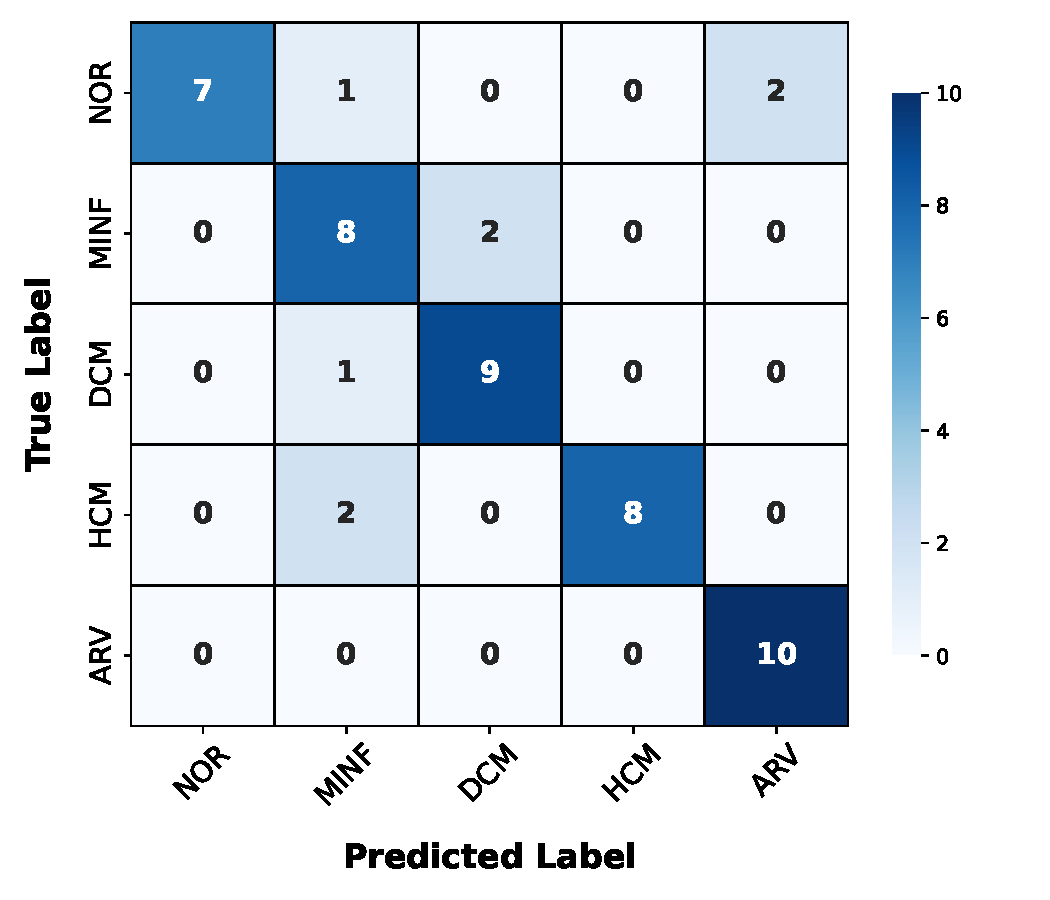
\includegraphics[width=0.45\linewidth]{img/56_fig_16a.pdf} &
    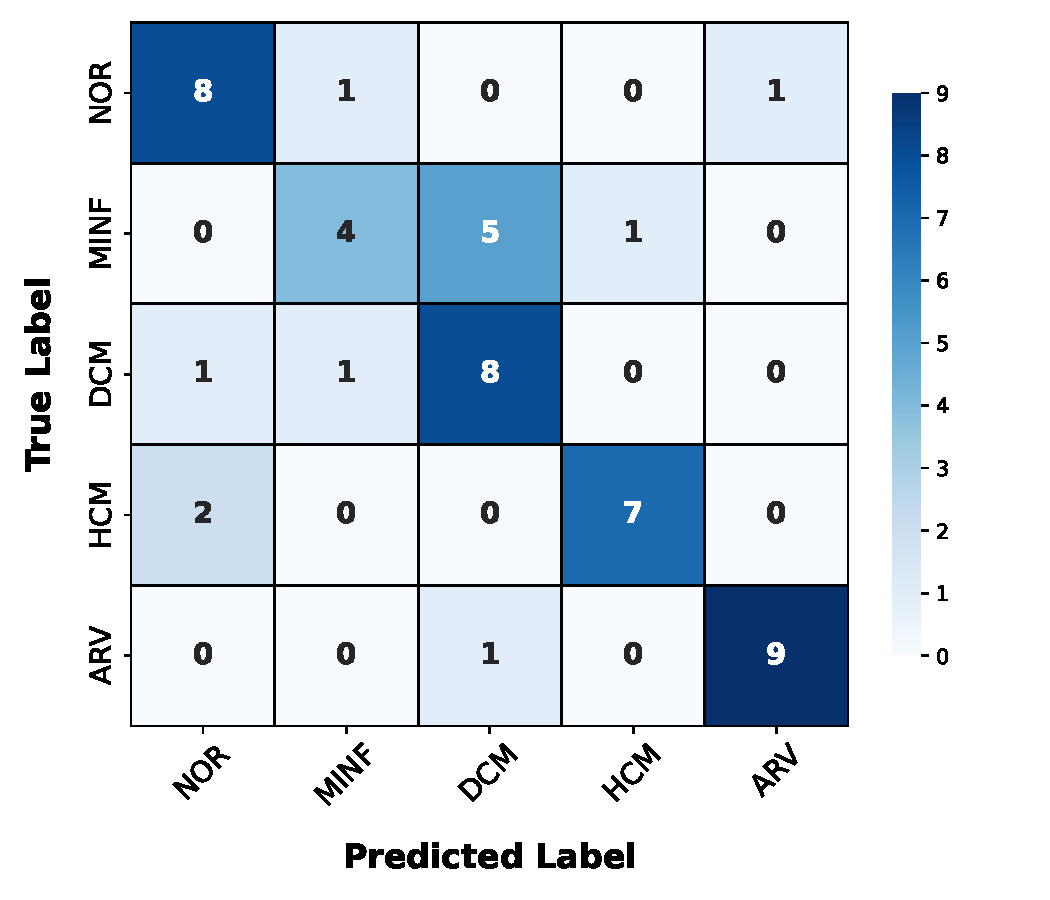
\includegraphics[width=0.45\linewidth]{img/56_fig_16b.pdf} \\
    \textbf{\textsf{(a)}} & \textbf{\textsf{(b)}}
\end{tabular}
\caption{Confusion matrices for multiclass classifiers using two architectures: \textbf{(a)} ResNet-50 and \textbf{(b)} ResNet-18, showcasing the classification performance across five classes, including NOR, MINF, DCM, HCM, and ARV.}
\label{fig:resnet50_confusion_matrix}
\end{figure}

Figure \ref{fig:cascade_confusion_matrices} depicts the confusion matrices for each classification stage, showing the number of correct, false positive, and false negative classifications.

\begin{figure}[ht]
\centering
\begin{tabular}{cccc}
    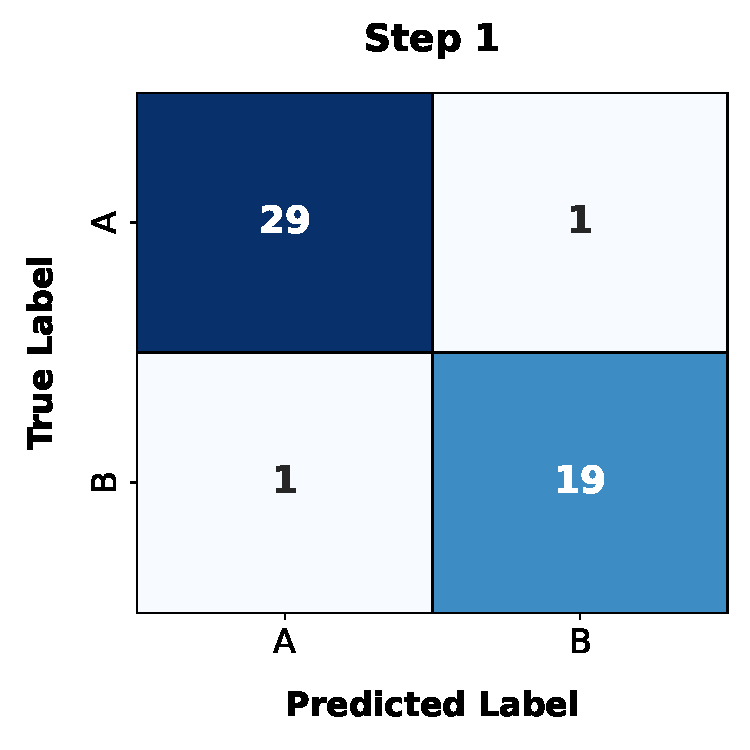
\includegraphics[width=0.22\linewidth]{img/56_fig_17_1.pdf} &
    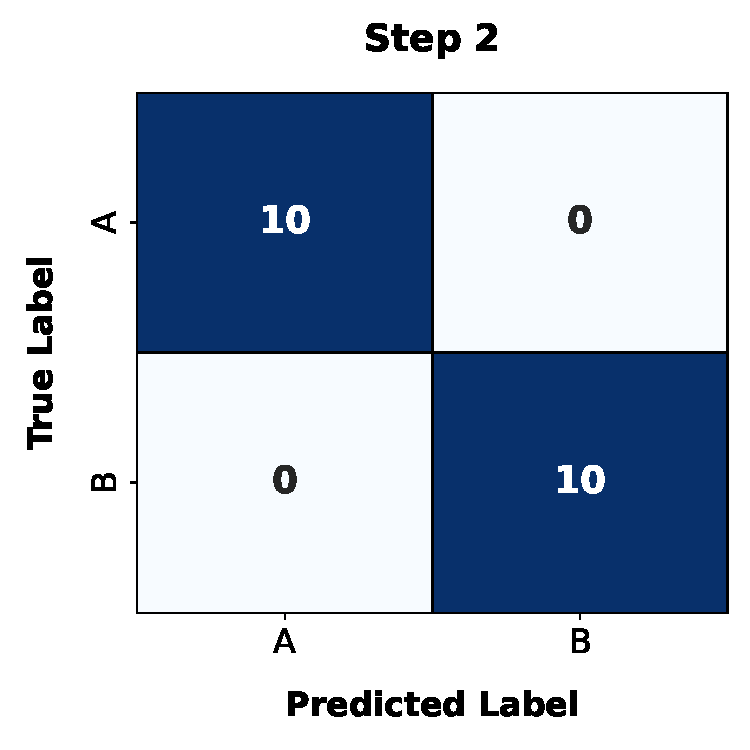
\includegraphics[width=0.22\linewidth]{img/56_fig_17_2.pdf} &
    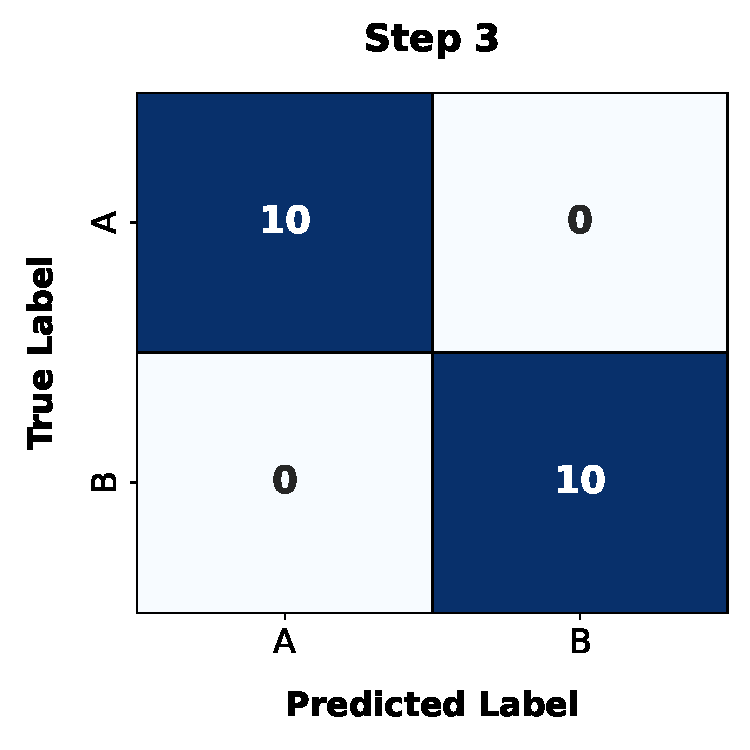
\includegraphics[width=0.22\linewidth]{img/56_fig_17_3.pdf} &
    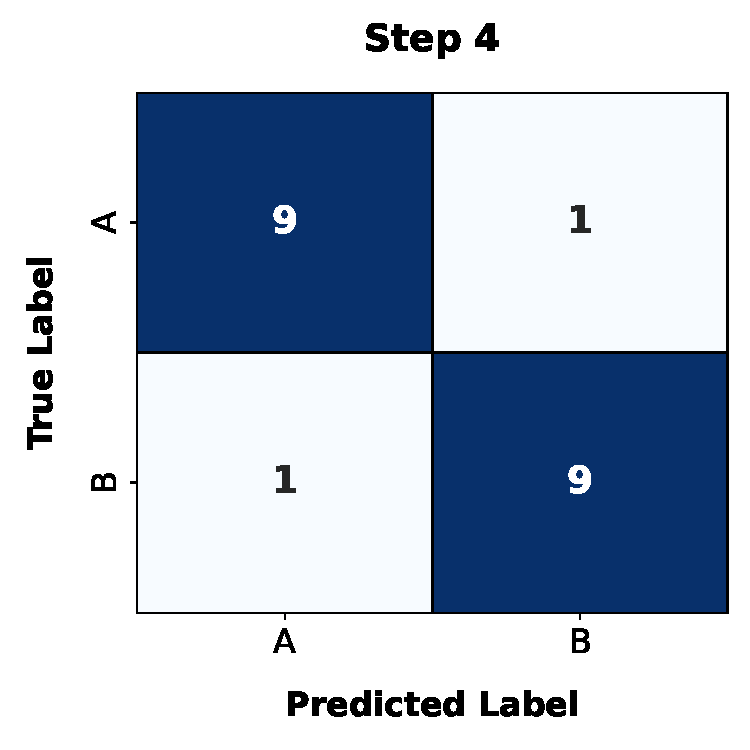
\includegraphics[width=0.22\linewidth]{img/56_fig_17_4.pdf} \\
    \textbf{\textsf{(a)}} & \textbf{\textsf{(b)}} & \textbf{\textsf{(c)}} & \textbf{\textsf{(d)}}
\end{tabular}
\caption{Confusion matrices, illustrating classification performance across sequential steps: \textbf{(a)} Step 1—Classifier 1, \textbf{(b)} Step 2—Classifier 2, \textbf{(c)} Step 3—Classifier 3, and \textbf{(d)} Step 4—Classifier 4, highlighting the accuracy and misclassifications for labels A and B at each step of the process.}
\label{fig:cascade_confusion_matrices}
\end{figure}

At the first classification stage, the model achieved an overall accuracy of 0.96, successfully separating LV pathologies (such as MINF, HCM, and DCM) from NOR and ARV. This result demonstrates the model’s high reliability in identifying major pathology groups, forming the foundation for further diagnostic refinement.

\Rone{\revtag{1}{12} % Action 12
The second classification stage showed a perfect accuracy of 1.0 (95\% CI: 0.94–1.00) in distinguishing NOR from ARV on the test set. While encouraging, this result on a small cohort may indicate potential for overfitting, and performance should be re-assessed on larger, more diverse datasets.
}

\Rone{\revtag{1}{12} % Action 12
The third classification stage also achieved 1.0 accuracy (95\% CI: 0.95–1.00) in Accuracy, Recall, and \({F_1}\)-score, effectively separating HCM from other LV pathologies such as MINF and DCM. This again highlights the model’s ability to recognize specific pathologies but warrants caution due to the limited sample size of the test set for these sub-classifications.
}

In the fourth classification stage, the model classified MINF and DCM with an Accuracy of 0.90. Although this result is slightly lower compared to previous stages, it still demonstrates satisfactory effectiveness in distinguishing these complex pathologies, which often overlap in visual and functional manifestations.

The proposed classification method was evaluated using several metrics: precision, recall, \({F_1}\)-score, and overall accuracy. These metrics were used for each of the four classification stages to assess the detection and separation of different heart pathologies. Table \ref{tab:cascade_classification_metrics} presents the classification results of the proposed model at each stage.

\begin{table}[ht]
\centering
\caption{Classification evaluation metrics for Classifiers 1–4 were obtained at steps 1–4, respectively, within the proposed classification method.}
\label{tab:cascade_classification_metrics}
\begin{tabular}{l lcccc}
\toprule
\textbf{Classifier} & \textbf{Classes} & \textbf{Precision} & \textbf{Recall} & \textbf{\({F_1}\)-score} & \textbf{Accuracy} \\
\midrule
Classifier 1 & NOR+ARV & 0.95 & 0.95 & 0.95 & \multirow{2}{*}{0.96} \\
 & MINF+HCM+DCM & 0.97 & 0.97 & 0.97 &  \\
\midrule
Classifier 2 & NOR & 1.00 & 1.00 & 1.00 & \multirow{2}{*}{1.00} \\
 & ARV & 1.00 & 1.00 & 1.00 &  \\
\midrule
Classifier 3 & HCM & 1.00 & 1.00 & 1.00 & \multirow{2}{*}{1.00} \\
 & MINF+DCM & 1.00 & 1.00 & 1.00 &  \\
\midrule
Classifier 4 & MINF & 0.90 & 0.90 & 0.90 & \multirow{2}{*}{0.90} \\
 & DCM & 0.90 & 0.90 & 0.90 &  \\
\bottomrule
\end{tabular}
\end{table}

Figure \ref{fig:cascade_roc_curves} illustrates the ROC curves for each classification stage, demonstrating the relationship between sensitivity (true positive rate) and specificity (false positive rate).

\begin{figure}[ht]
\centering
\begin{tabular}{cccc}
    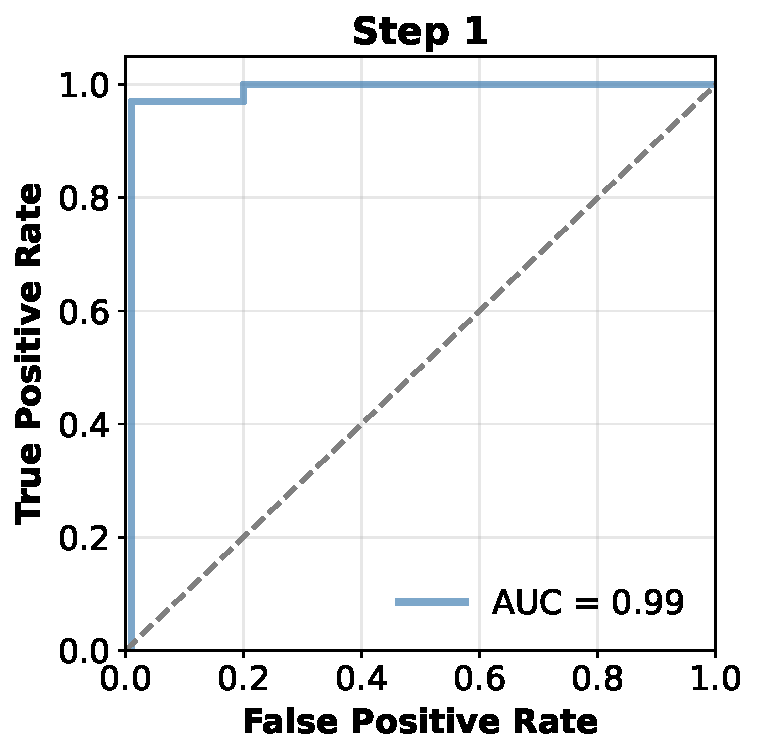
\includegraphics[width=0.22\linewidth]{img/56_fig_18_1.pdf} &
    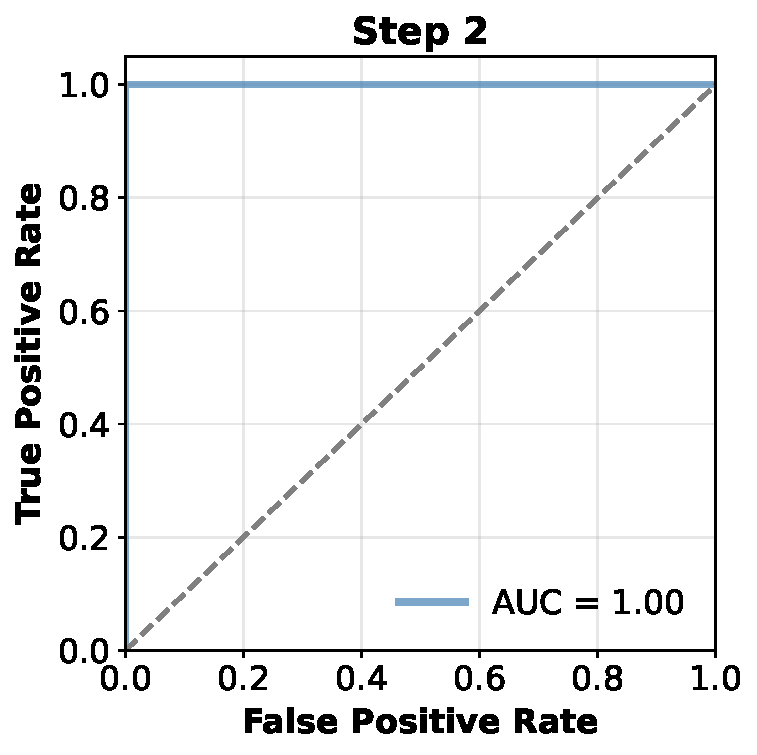
\includegraphics[width=0.22\linewidth]{img/56_fig_18_2.pdf} &
    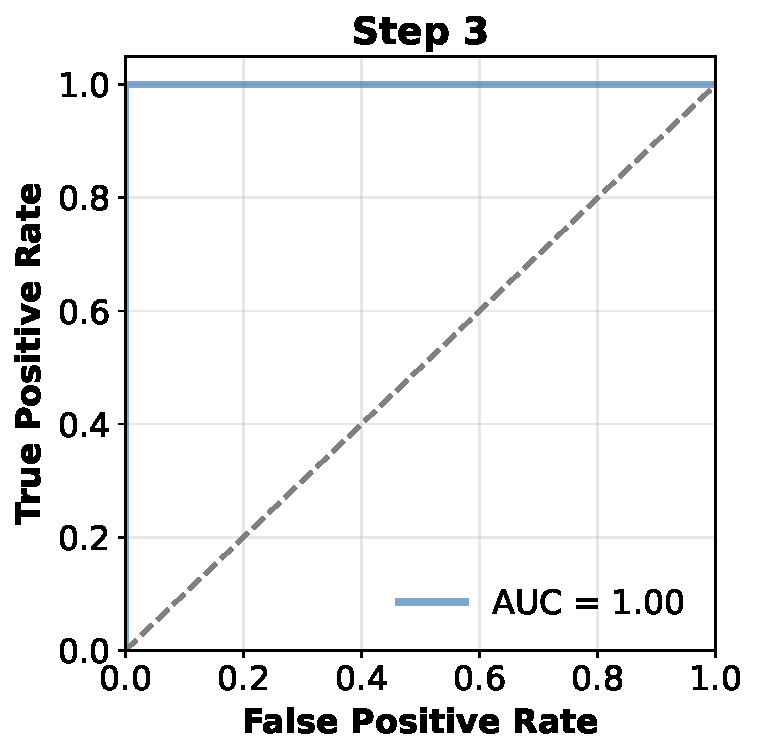
\includegraphics[width=0.22\linewidth]{img/56_fig_18_3.pdf} &
    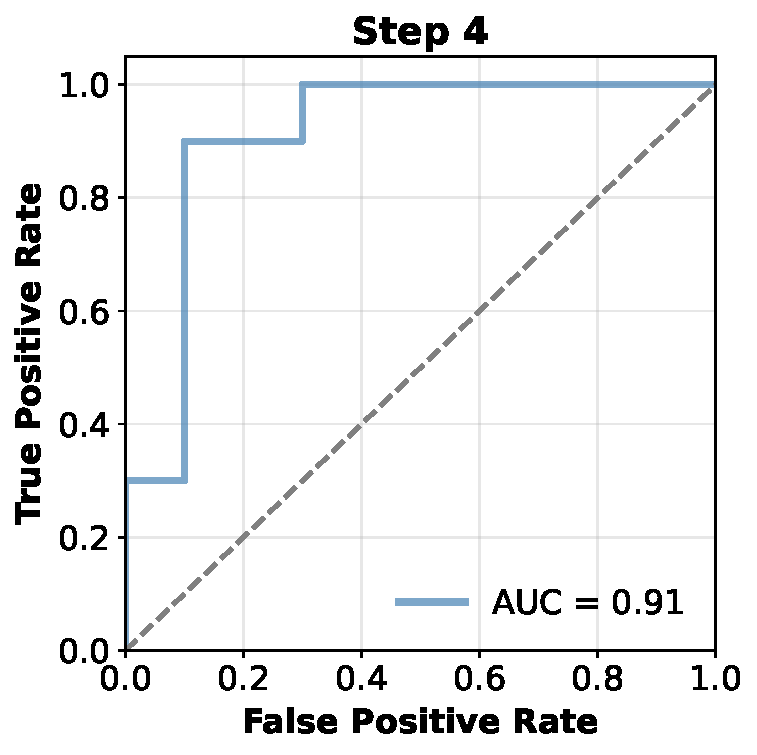
\includegraphics[width=0.22\linewidth]{img/56_fig_18_4.pdf} \\
    \textbf{\textsf{(a)}} & \textbf{\textsf{(b)}} & \textbf{\textsf{(c)}} & \textbf{\textsf{(d)}}
\end{tabular}
\caption{ROC curves for classification steps, showing the true positive rate versus false positive rate for \textbf{(a)} Step 1—Classifier 1 (AUC = 0.99), \textbf{(b)} Step 2—Classifier 2 (AUC = 1.00), \textbf{(c)} Step 3—Classifier 3 (AUC = 1.00), and \textbf{(d)} Step 4—Classifier 4 (AUC = 0.91).}
\label{fig:cascade_roc_curves}
\end{figure}

AUC for all classifiers confirms the high quality of the proposed approach. An AUC of 1.0 for stages 2 and 3 underscores the model’s ability to differentiate classes distinctly. Even in the final stage, where classification accuracy was 0.90, the AUC indicates high model quality in distinguishing MINF and DCM. The AUC is a crucial indicator of overall model quality as it reflects the model’s ability to differentiate between classes. \Rone{\revtag{1}{5}Model calibration was assessed via reliability diagrams (see Supplementary Fig. S6), showing low ECE and MCE values across all cascade stages, indicating that predicted probabilities are well-aligned with observed outcomes.}

A comparison of the overall accuracy of this method with the results from other studies is presented in Table \ref{tab:classification_comparison_sota}.

\begin{table}[ht]
\centering
\caption{Comparison of classification results with state-of-the-art methods by overall accuracy. Numbers in \textbf{bold} show the highest scores.}
\label{tab:classification_comparison_sota}
\begin{tabular}{ll}
\toprule
\textbf{Works} & \textbf{Accuracy} \\
\midrule
Zheng et. al. \cite{Zheng:2019} & 0.94 \\
Isensee et. al. \cite{Isensee:2018} & 0.94 \\
Khened et. al. \cite{Khened:2019} & 0.96 \\
Ours & \textbf{0.97} \\
\bottomrule
\end{tabular}
\end{table}

The overall accuracy \({A_{{\rm{gen}}}}\) of the method, defined by equation (14), is 97\%, surpassing the results of Khened et al. (96\%) and Zheng et al. (94\%), as well as Isensee et al. (94\%). This indicates the competitiveness of the method, especially considering that it consistently demonstrates high results at each classification stage, which is not always characteristic of other methods.

The experimental results clearly demonstrate the advantage of the multi-step approach, which enhances the accuracy and stability of classification even for complex heart pathologies. Multiclass classifiers based on ResNet-50 and ResNet-18 architectures, although standard tools in classification tasks, could not achieve comparable accuracy due to their limited adaptability in high-complexity data scenarios.

\Rtwo{\revtag{2}{3}\subsection*{External Validation on the M\&Ms Dataset}}
\Rtwo{\revtag{2}{3} % Action 9
To assess the generalizability of our ACDC-trained models, we performed inference on the external M\&Ms test set without any retraining or fine-tuning. This dataset introduces significant domain shift due to variations in scanner vendors, acquisition protocols, and patient populations. As shown in Extended Data Table \ref{tab:performance}, the hierarchical segmentation pipeline maintained strong, albeit reduced, performance. The mean Dice scores were lower compared to the internal ACDC test set, which is expected under domain shift, but remained competitive, demonstrating the model's robustness. The largest performance drop was observed for the RV, a structure known for high anatomical variability. Qualitative analysis of segmentation overlays confirmed that while most structures were correctly delineated, errors were more frequent at the apical/basal slices and in scans from the vendor not present in the ACDC dataset. These results underscore the value of our hierarchical approach while also highlighting the persistent challenge of out-of-domain generalization in cardiac MRI analysis.
}

\subsection*{Results of the Interpretation Method}

In this subsection, we present examples of interpreting the classification results using the proposed interpretation method. The features introduced in the interpretation model for individual pathologies were utilized to analyze results. Fifty patients from the test dataset (10 for each class) were analyzed. Below, we provide an example analysis for a specific patient in each class.

\subsubsection*{Dilated Cardiomyopathy (DCM)}

The hallmark of DCM is significant enlargement of the LV and reduced contractility. As shown in Figure \ref{fig:dcm_visualization}, the LV ED volume (feature \(o_1^1\)) is notably increased (222.59 ml) compared to normal values (100–200 ml for men).

\begin{figure}[ht]
\centering
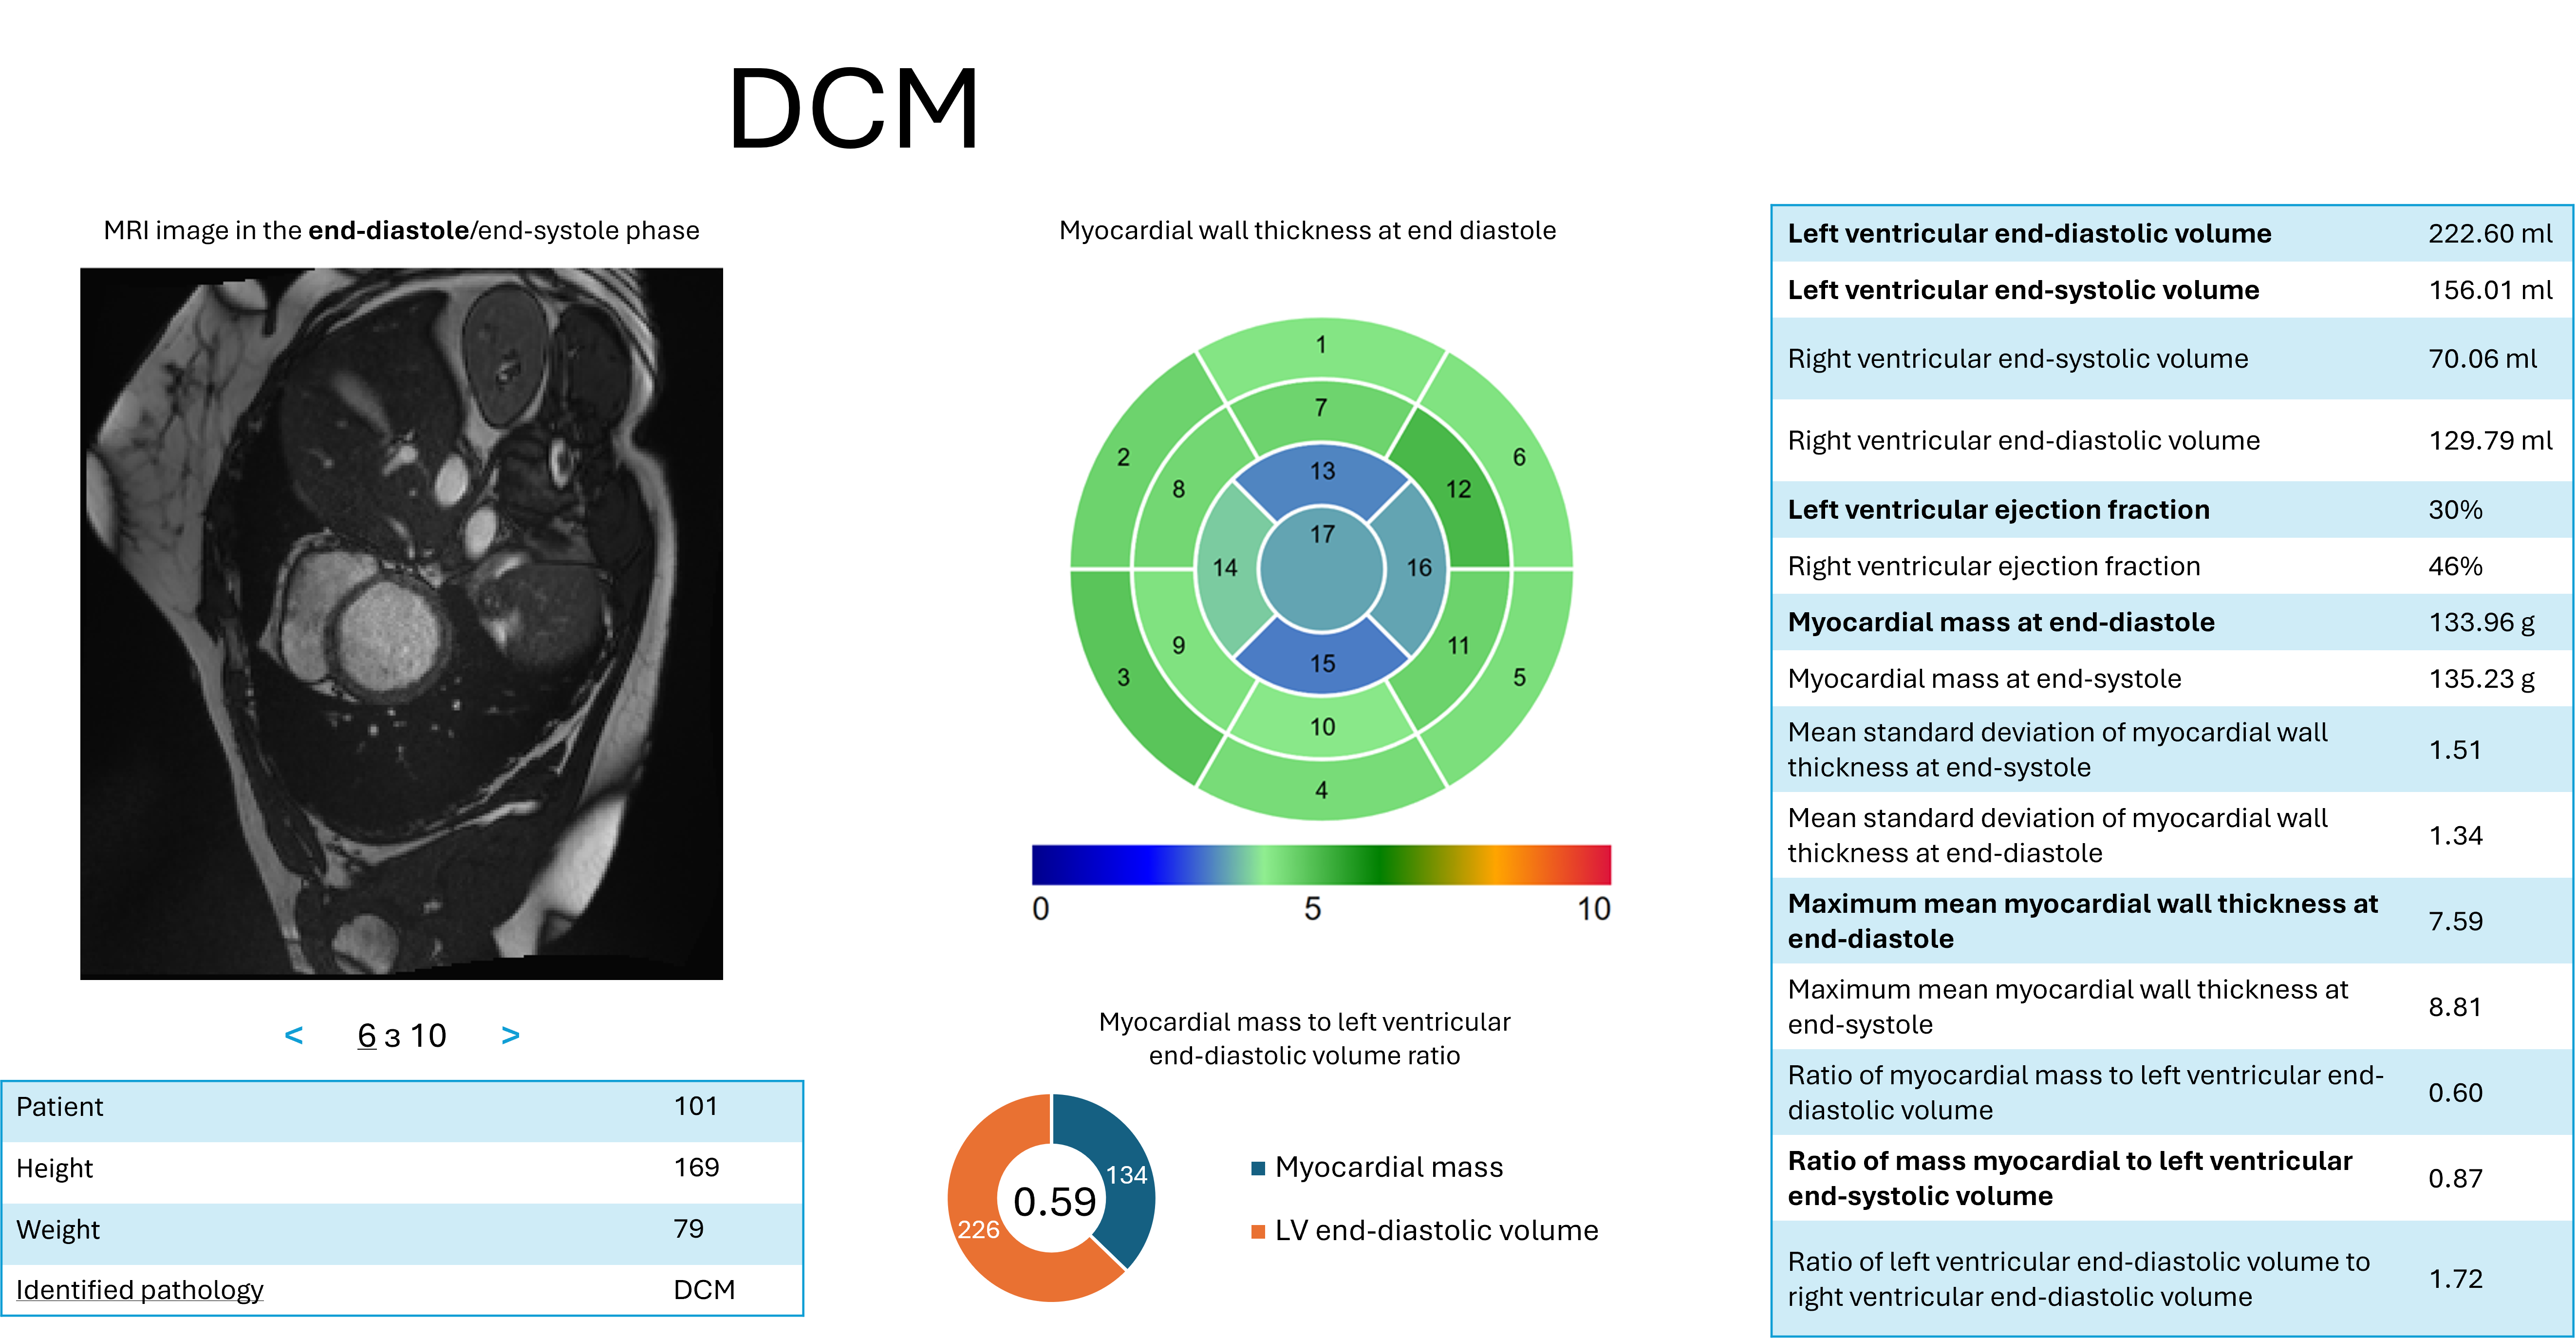
\includegraphics[width=0.9\linewidth]{img/56_fig_19_DCM.png}
\caption{Visualization of DCM, highlighting significant LV enlargement and reduced systolic function, accompanied by detailed metrics, including LV volumes, myocardial mass, ejection fractions, and wall thicknesses, to provide a comprehensive analysis of the pathological condition.}
\label{fig:dcm_visualization}
\end{figure}

The ES volume (feature \(o_2^1\)) is likewise high (156.01 ml), while the LV ejection fraction (feature \(o_3^1\)) drops to 29\% (normally 55–70\%). Although the myocardial mass (feature \(o_4^1\)) remains around 133.96 g (almost normal), the ratio of myocardial mass to ED volume (feature \(o_5^1\)) is only 0.6, confirming ventricular dilation. On the myocardium model, certain LV wall segments (feature \(o_6^1\)) appear thinner than usual, reinforcing the DCM diagnosis.

\subsubsection*{Hypertrophic Cardiomyopathy (HCM)}

HCM typically presents with asymmetric hypertrophy and uneven wall thickness (see Supplementary Fig. S2 in Appendix A). In Supplementary Fig. S2, the LV ES volume (feature \(o_1^2\)) is relatively small (27.05 ml), suggesting robust contractility. The ejection fraction (feature \(o_2^2\)) is elevated at 84\%, while the ratio of myocardial mass to ES volume (feature \(o_3^2\)) reaches 6.05, reflecting substantial thickening. On the myocardium model, certain regions (features \(o_4^2\), \(o_5^2\), \(o_6^2\)) appear excessively hypertrophied, confirming an HCM pattern.

\subsubsection*{Myocardial Infarction with Altered LV ejection fraction (MINF)}

It often manifests as reduced LV ejection fraction, sometimes alongside myocardial inflammation best detected with specialized imaging (Supplementary Fig. S3 in Appendix A). In Supplementary Fig. S3, the patient’s ejection fraction (feature \(o_2^3\)) is 26\%, significantly below normal. The LV ED volume (feature \(o_1^3\)) is 178.17 ml, close to the upper limit, and myocardial mass (feature \(o_3^3\)) is 182.44 g. The maximum wall thickness (feature \(o_4^3\)) hovers at the high end of normal (12.57 mm), and the mean standard deviation of wall thickness (feature \(o_5^3\)) is 2.06 mm, indicating uneven edema.

\subsubsection*{Abnormal right ventricle (ARV)}

ARV features RV dilation and decreased RV ejection fraction (see Supplementary Fig. S4 in Appendix A). In Supplementary Fig. S4, the RV ED volume (feature \(o_1^4\)) is markedly high (219.58 ml), far above typical values (80–120 ml). The RV ES volume (145.48 ml) is also elevated, leaving an ejection fraction (feature \(o_2^4\)) at 34\%. By contrast, the LV remains near normal volumes, though the ratio of LV to RV ED volumes (feature \(o_3^4\)) is a low 0.72, confirming pronounced RV dominance.

\subsubsection*{Normal State (NOR)}

In Supplementary Fig. S5 in Appendix A, the patient’s LV exhibits near-normal ES volume (feature \(o_1^5\)) of 41.75 ml, ED volume (feature \(o_2^5\)) of 125.51 ml, and an ejection fraction (feature \(o_4^5\)) of 67\%, all consistent with healthy cardiac function. The RV volumes and ejection fraction lie within acceptable limits, and myocardial thickness remains stable. Together, these findings confirm the absence of significant pathology.

Overall, each pathology displays a unique profile of volumetric and functional changes: DCM is dominated by LV dilation; HCM shows asymmetric hypertrophy; MINF frequently reveals reduced EF with tissue irregularities; ARV reflects severe RV enlargement; and NOR remains within healthy ranges. The proposed interpretation approach clarifies each classification outcome in clinical terms by highlighting the most relevant quantitative features and visual cues.

\subsection*{Limitations of the Proposed Methods}

Although the proposed methods for myocardium segmentation in the LV and RV show promise, certain limitations require attention.

Firstly, the model’s performance can deteriorate significantly when processing low-quality MRI scans. This issue is especially noticeable when parts of the myocardium or ventricles are not fully visible, resulting in incorrect segmentations or complete omission of these regions. The model heavily relies on detecting differences between the target structures and surrounding tissues; thus, poor image quality seriously affects accuracy.

Another challenge arises when image brightness levels are too low or too high (Figures \ref{fig:partial_myocardium_visualization}a-b). In such cases, the model may have difficulty correctly defining the boundaries of cardiac structures, resulting in poorly delineated segmentations. This occurs because areas with insufficient or excessive brightness lose crucial detail, negatively affecting model training quality.

\begin{figure}[!htbp]
\centering
\begin{tabular}{cccc}
    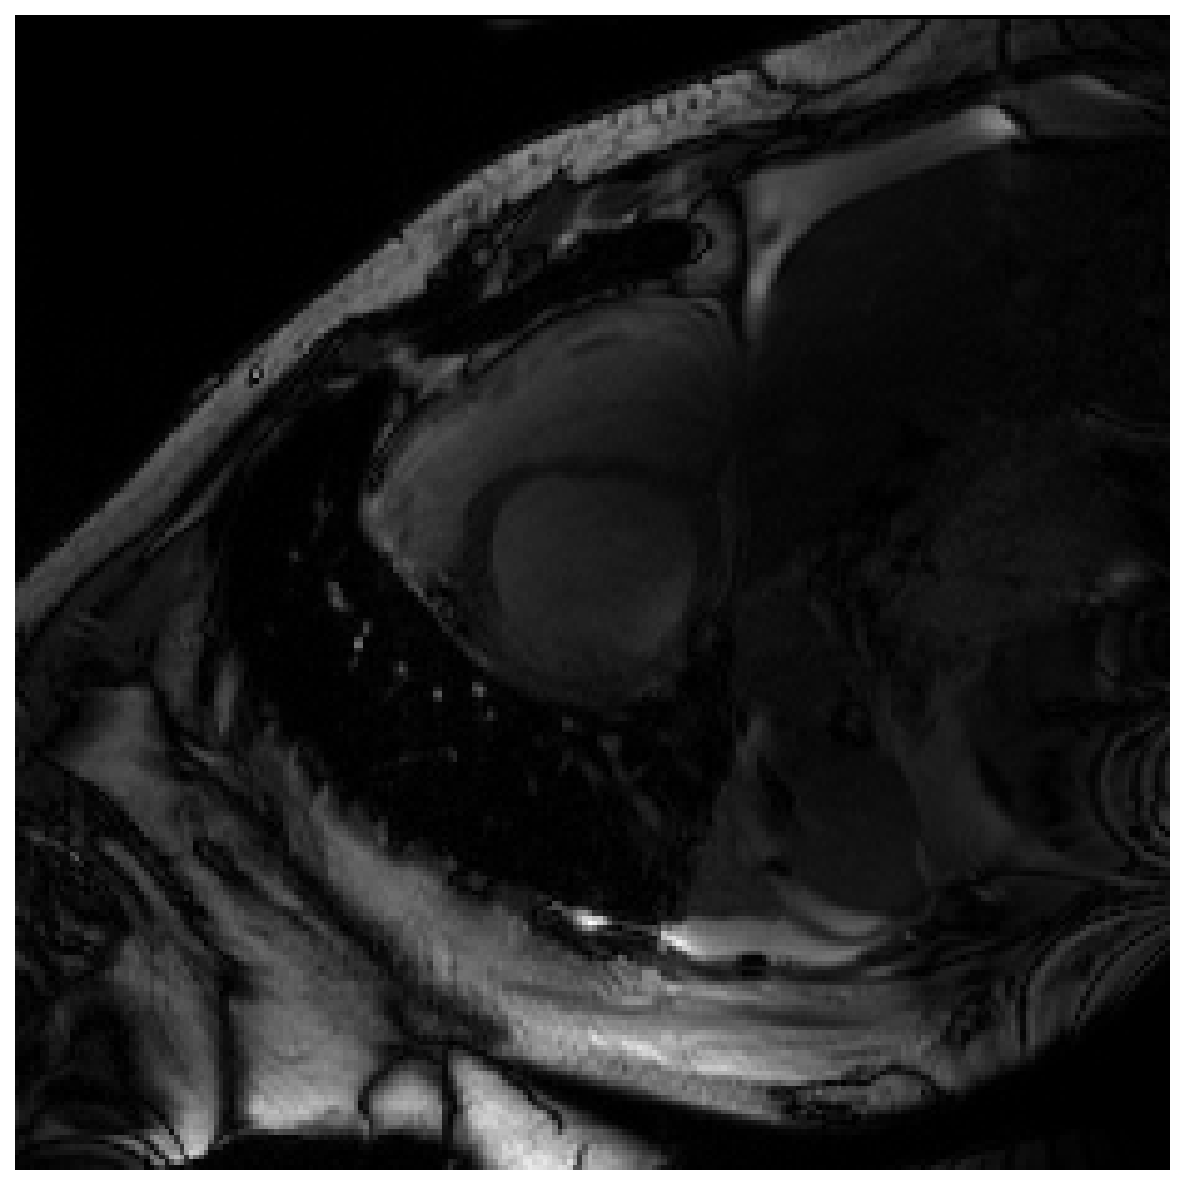
\includegraphics[width=0.22\linewidth]{img/56_fig_20a.pdf} &
    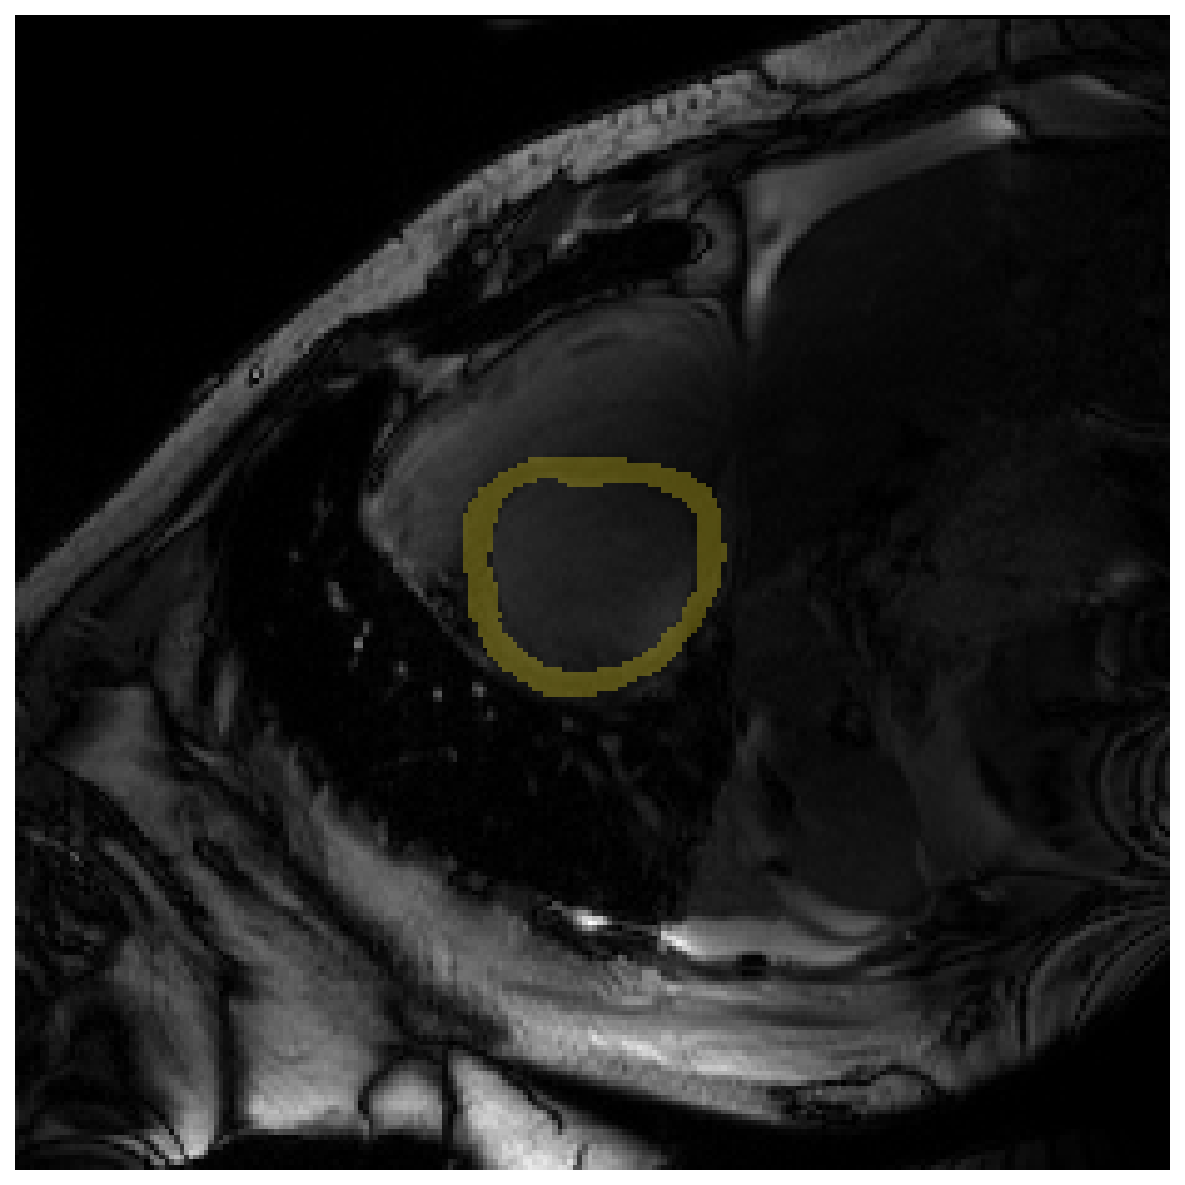
\includegraphics[width=0.22\linewidth]{img/56_fig_20b.pdf} &
    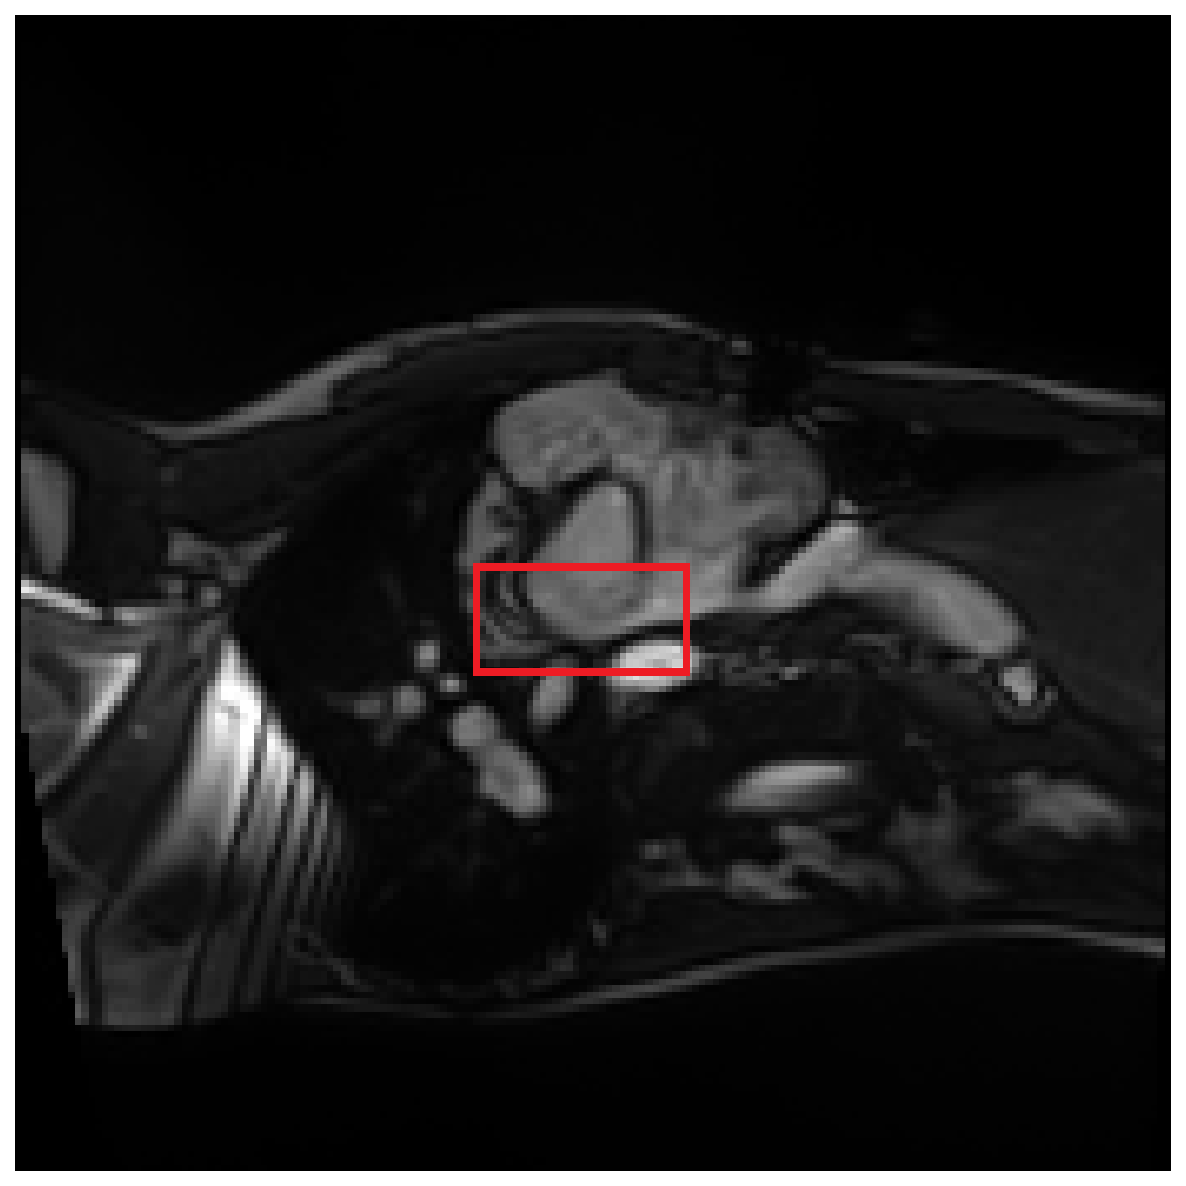
\includegraphics[width=0.22\linewidth]{img/56_fig_20c.pdf} &
    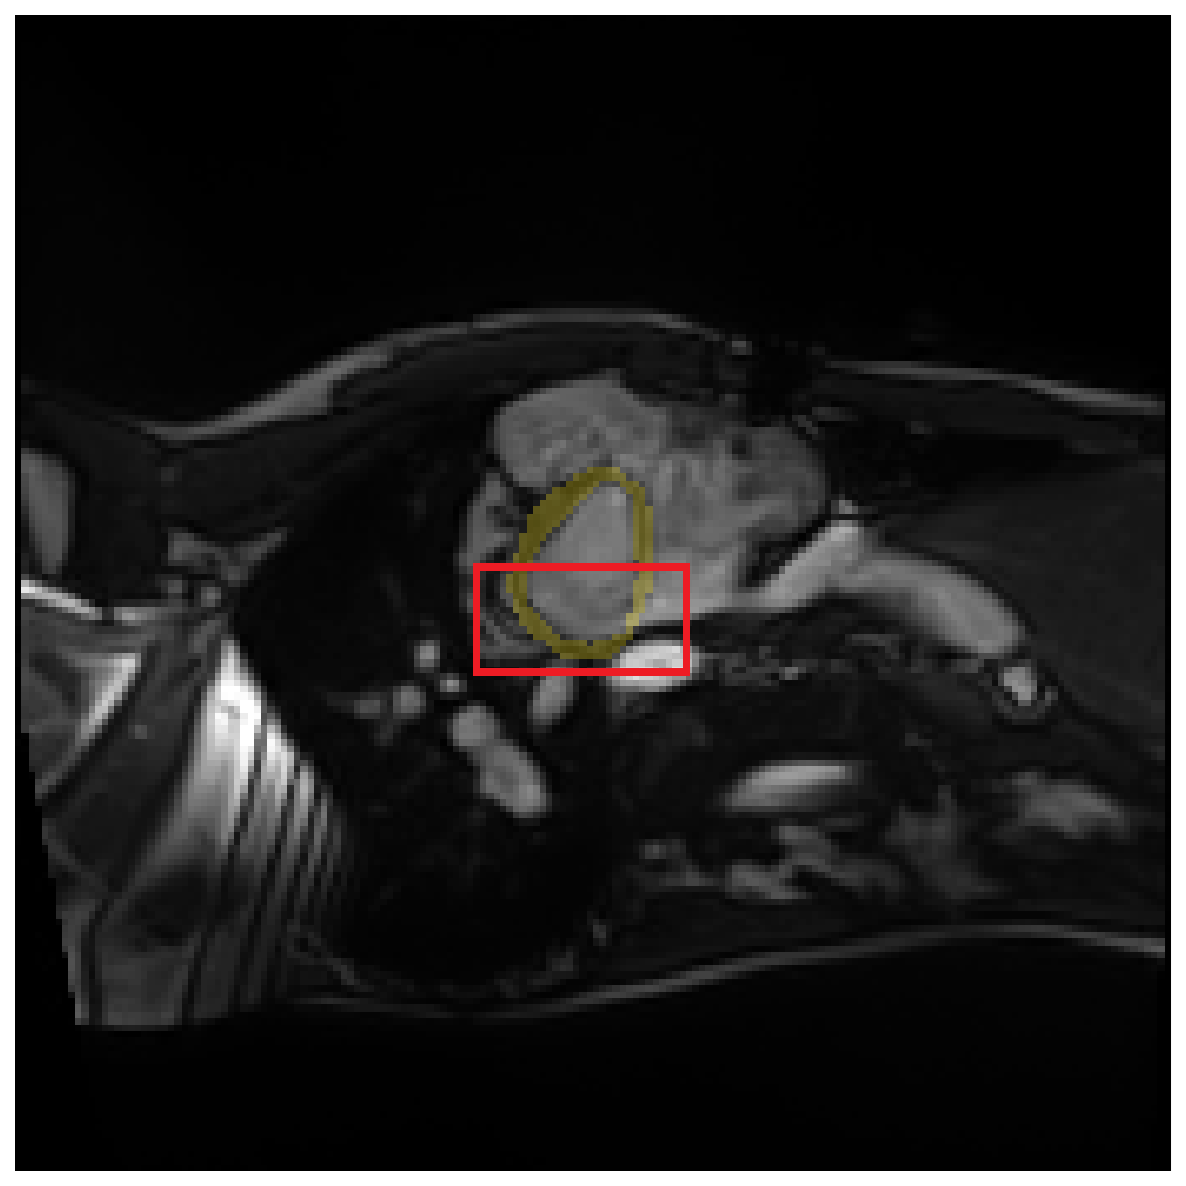
\includegraphics[width=0.22\linewidth]{img/56_fig_20d.pdf} \\
    \textbf{\textsf{(a)}} & \textbf{\textsf{(b)}} & \textbf{\textsf{(c)}} & \textbf{\textsf{(d)}}
\end{tabular}
\caption{Illustrated challenges in cardiac MRI analysis due to insufficient image quality. In \textbf{(a)} and \textbf{(b)}, low brightness affects the delineation of cardiac structures, particularly the myocardium (highlighted in yellow), leading to poor segmentation. In \textbf{(c)} and \textbf{(d)}, partial myocardium visualization issues (also highlighted in yellow), caused by slice timing, affect the model's accuracy, as shown by the incomplete lower myocardium (marked in a red rectangle).}
\label{fig:partial_myocardium_visualization}
\end{figure}

Furthermore, the training data used to develop the models lacked sufficient examples of certain pathological conditions, such as cardiomyopathy or noncompaction myocardium. This shortage of samples may reduce the model’s ability to generalize to more complex conditions, thus affecting its reliability in clinical settings.

\Rtwo{\revtag{2}{2} % Action 12
While our slice-position–aware refinement module improves segmentation at the ventricular extremes (Supplementary Table S1), challenges remain. In some images, specific segments fail to visualize or only partially appear, often due to slice timing (e.g., capturing the moment the mitral or tricuspid valve is opening). The model may still produce inaccurate results if segments are not clearly visible. Figures \ref{fig:partial_myocardium_visualization}c-d show a case where the lower myocardium is poorly visualized but is still marked in the mask. Such ground-truth ambiguities can teach the network to erroneously fill these areas in similar cases, a residual error our current method does not fully resolve.
}

The proposed methods were validated exclusively on the ACDC dataset. While this is a standard and well-annotated benchmark, validating the model's generalizability and robustness on other publicly available short-axis cardiac MRI datasets, such as the M\&Ms 2020 challenge dataset \cite{Campello:2021}, would be a valuable next step. Such multi-dataset validation is planned for future work to ensure the methods perform reliably across different scanners, imaging protocols, and patient populations.

Hence, although the approach is reliable under ideal conditions, its effectiveness strongly depends on the quality of the input data. Extra caution is needed when working with low-quality images or rare pathologies, as these factors can reduce accuracy and make the model less dependable in critical diagnostic situations.

\subsection*{Discussion}

Each stage of the proposed multi-stage MRI segmentation method was examined during the experiments—from processing the original images to a comprehensive approach that includes localization, decomposition, and postprocessing. Each step contributed to improved accuracy in segmenting cardiac structures, as confirmed by the Dice coefficient for ED and ES phases. In the initial stage, segmenting the original images without localization or decomposition resulted in limited accuracy due to the influence of background noise and structural overlap. The final stage, which encompassed localization, mask decomposition, and postprocessing, achieved the best results. The proposed method effectively removed residual artifacts, smoothed contours, and improved the consistency of masks relative to expert annotations. This outcome confirmed the effectiveness of the proposed method, which combines all key processing steps: localization, decomposition, and postprocessing.

The proposed segmentation method achieved high accuracy: the Dice coefficient for the LV reached 0.974 in the ED phase and 0.940 in the ES phase. For the RV, the corresponding values were 0.947 and 0.915. The LV myocardium was segmented at 0.896 accuracy in diastole and 0.920 in systole, making it a promising tool for clinical applications and further research. According to a practicing cardiologist, 97.73\% of the masks are satisfactory and of sufficient quality for medical analysis. The remaining 2.27\% have poorer results mainly due to the low quality of the input images—specifically, suboptimal cardiac visualization owing to low resolution or image artifacts such as blurring (caused by patient movement during the MRI examination), low brightness, or low contrast (stemming from the MRI equipment’s limitations or technical challenges in a particular patient’s examination).

The introduced cascade classification method for detecting cardiac pathologies in MRI scans also shows high accuracy. Using separate classifiers at each stage provided considerable precision and consistency, even for challenging cases. The model achieved an overall accuracy of 97\%, surpassing most current methods presented in the literature. Further experiments using multiclass classifiers ResNet-50 and ResNet-18 highlighted their limitations: ResNet-50 reached 84\% accuracy, indicating difficulties in distinguishing similar classes such as MINF and DCM, while ResNet-18 (with fewer parameters) scored even lower at 72\%, underscoring its insufficient capacity for complex classification tasks. These findings emphasize the advantages of the proposed step-by-step approach, which effectively accommodates each class’s specific characteristics. Comparisons with contemporary methods further confirmed the competitive nature of the proposed technique. Its high accuracy and adaptability make it promising for clinical integration, where robust classification performance and the ability to handle complex medical data are crucial.

\Rtwo{\revtag{2}{2}A known challenge in cardiac MRI segmentation is the accurate delineation of apical and basal slices, where anatomical boundaries are often less distinct and partial volume effects are more pronounced. While our method does not incorporate algorithms explicitly designed for these slices, the proposed multi-stage approach inherently improves their segmentation. By first localizing the heart, the model reduces the influence of surrounding tissues and background noise. Subsequently, using separate, specialized networks for the LV, RV, and myocardium allows each model to learn the specific morphological features of its target structure, enhancing sensitivity even in low-contrast regions. Finally, post-processing helps refine contours and remove small, erroneous segmentations common in these challenging edge slices. Our slice-position-aware refinement module with its shape-prior further improves performance, as demonstrated by the stratified results (see Supplementary Table S1). This hierarchical strategy contributes to a more robust and accurate segmentation across the entire ventricular stack, including the difficult apical and basal regions.}

\Rthree{\revtag{3}{7}\subsubsection*{Papillary Muscles and Clinical Indices}}
\Rthree{\revtag{3}{7} % Action 13
The handling of papillary muscles significantly influences the calculation of LV mass and ejection fraction. Our default policy is to \emph{exclude} papillary muscles from the LV cavity volume and myocardial mass computations to maintain consistency with common clinical reporting standards. We performed a sensitivity analysis to quantify the impact of this choice, detailed in Extended Data Table \ref{tab:papillary_sensitivity}. The results show that including papillary muscles in the myocardial mass increases the calculated mass and slightly alters the ejection fraction. We recommend the exclusion policy for standardization, but users of the model can adapt this choice based on institutional protocol.
}

The designed method for interpreting results allows a clear, structured presentation of medical data analysis outcomes. Adaptive visualization techniques—such as the 17-segment model, circular charts, and numerical values—offer clinicians an intuitive grasp of the results. This presentation style simplifies the diagnostic process and facilitates the incorporation of the findings into clinical practice.

\section*{Conclusions}

This study introduces a set of novel methods for processing and evaluating cardiac MRI scans with higher precision and clarity. First, region extraction was refined by combining image resizing, specialized feature extraction layers, and further enhancements like postprocessing to smooth boundaries and minimizing artifacts. These steps boosted segmentation accuracy for the LV, RV, and myocardium. Second, classification was performed by separating classes into multiple phases, allowing the model to specialize in distinguishing particular sets of heart conditions. This phased approach achieved a high overall accuracy, even for challenging pathologies such as those characterized by overlapping visual cues. Third, a metric-based interpretation scheme was developed, converting raw outputs into understandable clinical parameters, including ventricular volumes, wall thickness, and ejection fractions. By highlighting these features, the system provides transparency for physicians who must verify how diagnoses align with known cardiac metrics.

The numerical improvements are persuasive. Specifically, a Dice coefficient of 0.974 for the LV, 0.947 for the RV, and 0.896–0.920 for the myocardium underscore the effectiveness of the proposed region delineation. Classification benchmarks also showed consistently high performance (97\%), far outpacing established reference architectures. However, several limitations remain. Specifically, low-quality MRIs, i.e., poor resolution, motion artifacts, and brightness imbalances, can undermine segmentation and classification results. Moreover, limited training examples for certain rare pathologies hamper the model’s generalizability, suggesting additional data-gathering efforts are needed.

Future prospects include validating these methods across more diverse imaging protocols and rare cardiac conditions to ensure consistent performance. Furthermore, investigations into semi-supervised or self-supervised learning techniques may improve accuracy and reduce reliance on extensive annotations.

\Rthree{\revtag{3}{2}\section*{Data availability}}
\Rthree{\revtag{3}{2} % Action 15
The ACDC dataset\cite{Bernard:2018} is publicly accessible for research under the challenge’s access terms (the challenge website is provided in the Supplementary Information). External validation used the M\&Ms dataset\cite{Campello:2021}, available from the organizers under their specified terms. Preprocessed data derivatives generated in this study, including cropped image stacks and segmentation masks, along with evaluation scripts, will be released with the code. The full, pre-processed dataset containing the specific image crops and segmentation masks generated and used for training and testing in this study is available at the following repository: \url{https://drive.google.com/drive/folders/1qBpZR2LvrWwW70OLAJbOx74eWBlxtkA2?usp=sharing} (2025).
}

\Rone{\revtag{1}{11}\section*{Code availability}}
\Rone{\revtag{1}{11} % Action 16
All code for preprocessing, model training, and evaluation will be released in a versioned repository with a tagged release, comprehensive documentation, and an environment file to ensure reproducibility. We provide a one-command inference script, fixed random seeds, and exact library versions. The source code is available at: \url{https://github.com/vitalii-slobodzian/cardiac-mri-analysis/tree/main} (2025).
}

\bibliography{sample}

\section*{Author contributions statement}
V.S. and O.B. conceived and conducted the experiments, V.S., O.B., and L.K. validated the results, V.S., O.B., and P.R. made formal analysis, V.S. did investigation, P.R. and L.K. conducted data curation, V.S. and O.B. prepared the draft of the manuscript, P.R., L.K. and I.K. reviewed and edited the manuscript, V.S. and P.R. made visualizations, I.K. and O.B. provided the supervision. All authors reviewed, corrected, and approved the paper.

\section*{Additional information}

\Rthree{\revtag{3}{2}\textbf{Compliance with ethical standards:} % Action 17
We used de-identified, publicly available data from the ACDC and M\&Ms challenges; no new institutional review board approval was required for this retrospective study. Our use of the data complied with the respective terms of each challenge.
}
\textbf{Competing interests:} The authors declare no competing interests.

\appendix
\section*{Appendix A}

\renewcommand{\thefigure}{S\arabic{figure}}
\setcounter{figure}{0}

\begin{figure}[!htbp]
\centering
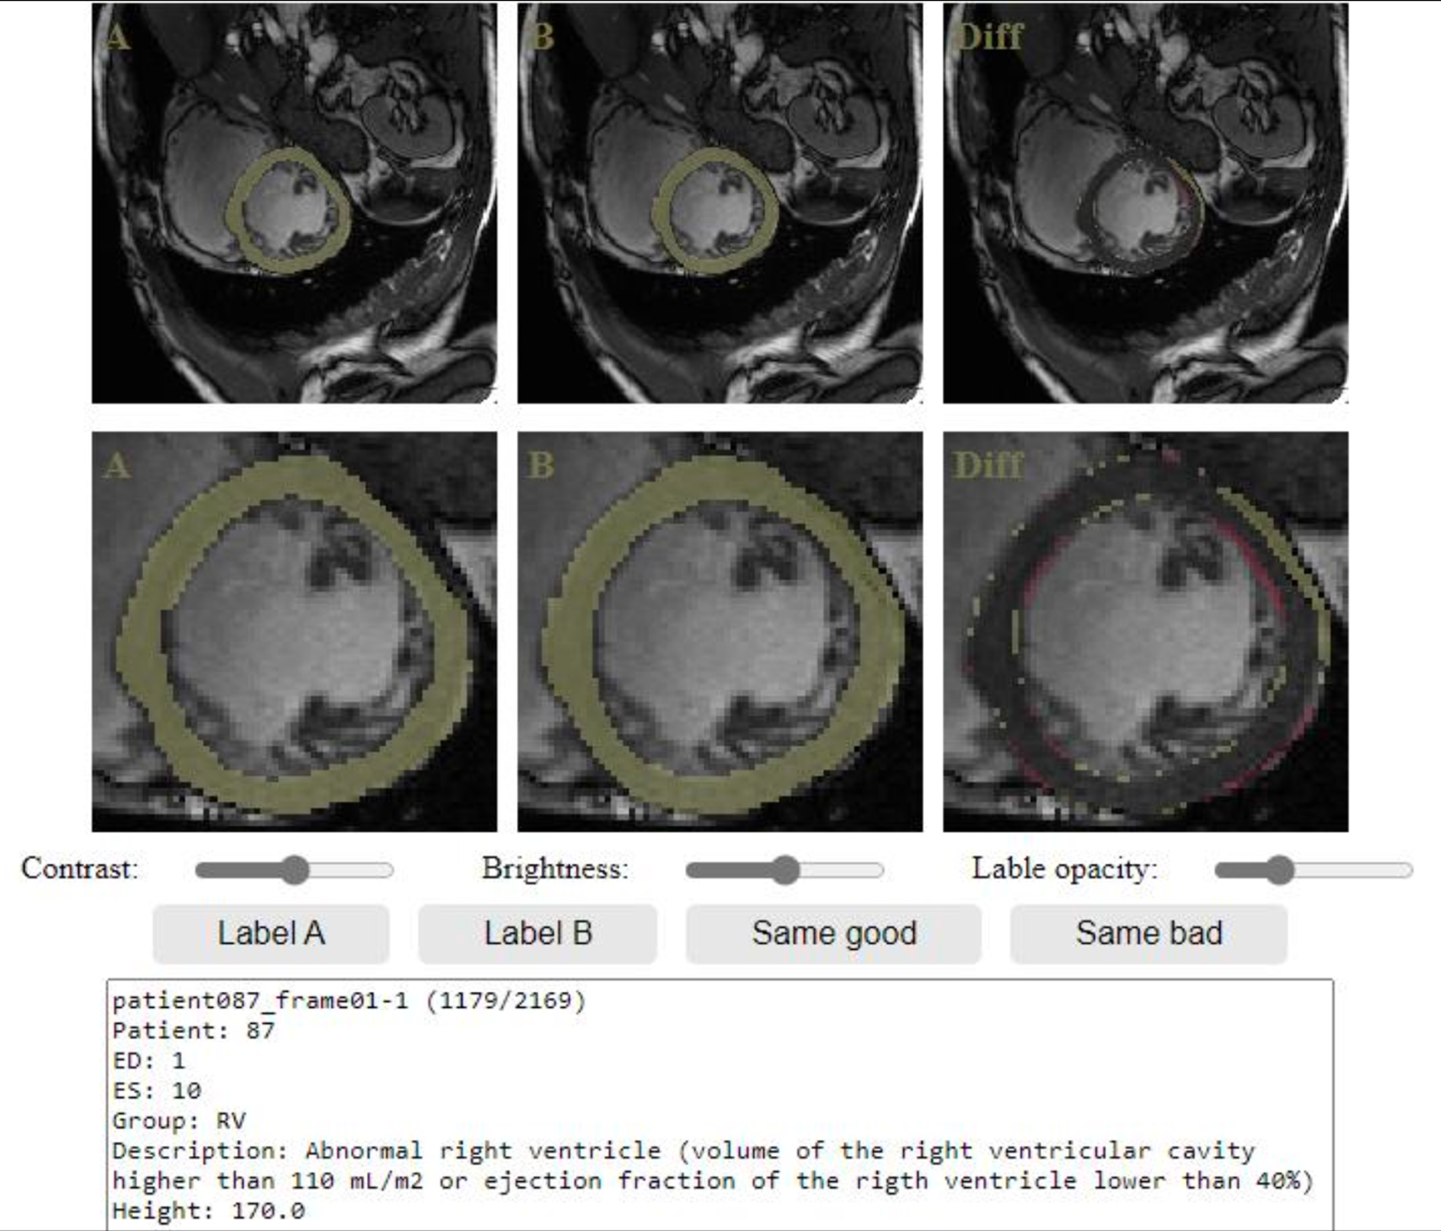
\includegraphics[width=0.8\linewidth]{img/56_fig_s1_interface.png}
\caption{The user interface of the custom software application developed for expert validation of segmentation masks. The interface allows a side-by-side comparison of two anonymized masks (Mask A and Mask B) overlaid on the cardiac MRI scan. The validating clinician can adjust image brightness and contrast, control mask opacity, and zoom in on specific regions. Based on this detailed visual analysis, the expert selects one of four options to grade the relative accuracy of the masks, ensuring an objective and thorough evaluation process.}
\label{fig:validation_app}
\end{figure}

\begin{figure}[!htbp]
\centering
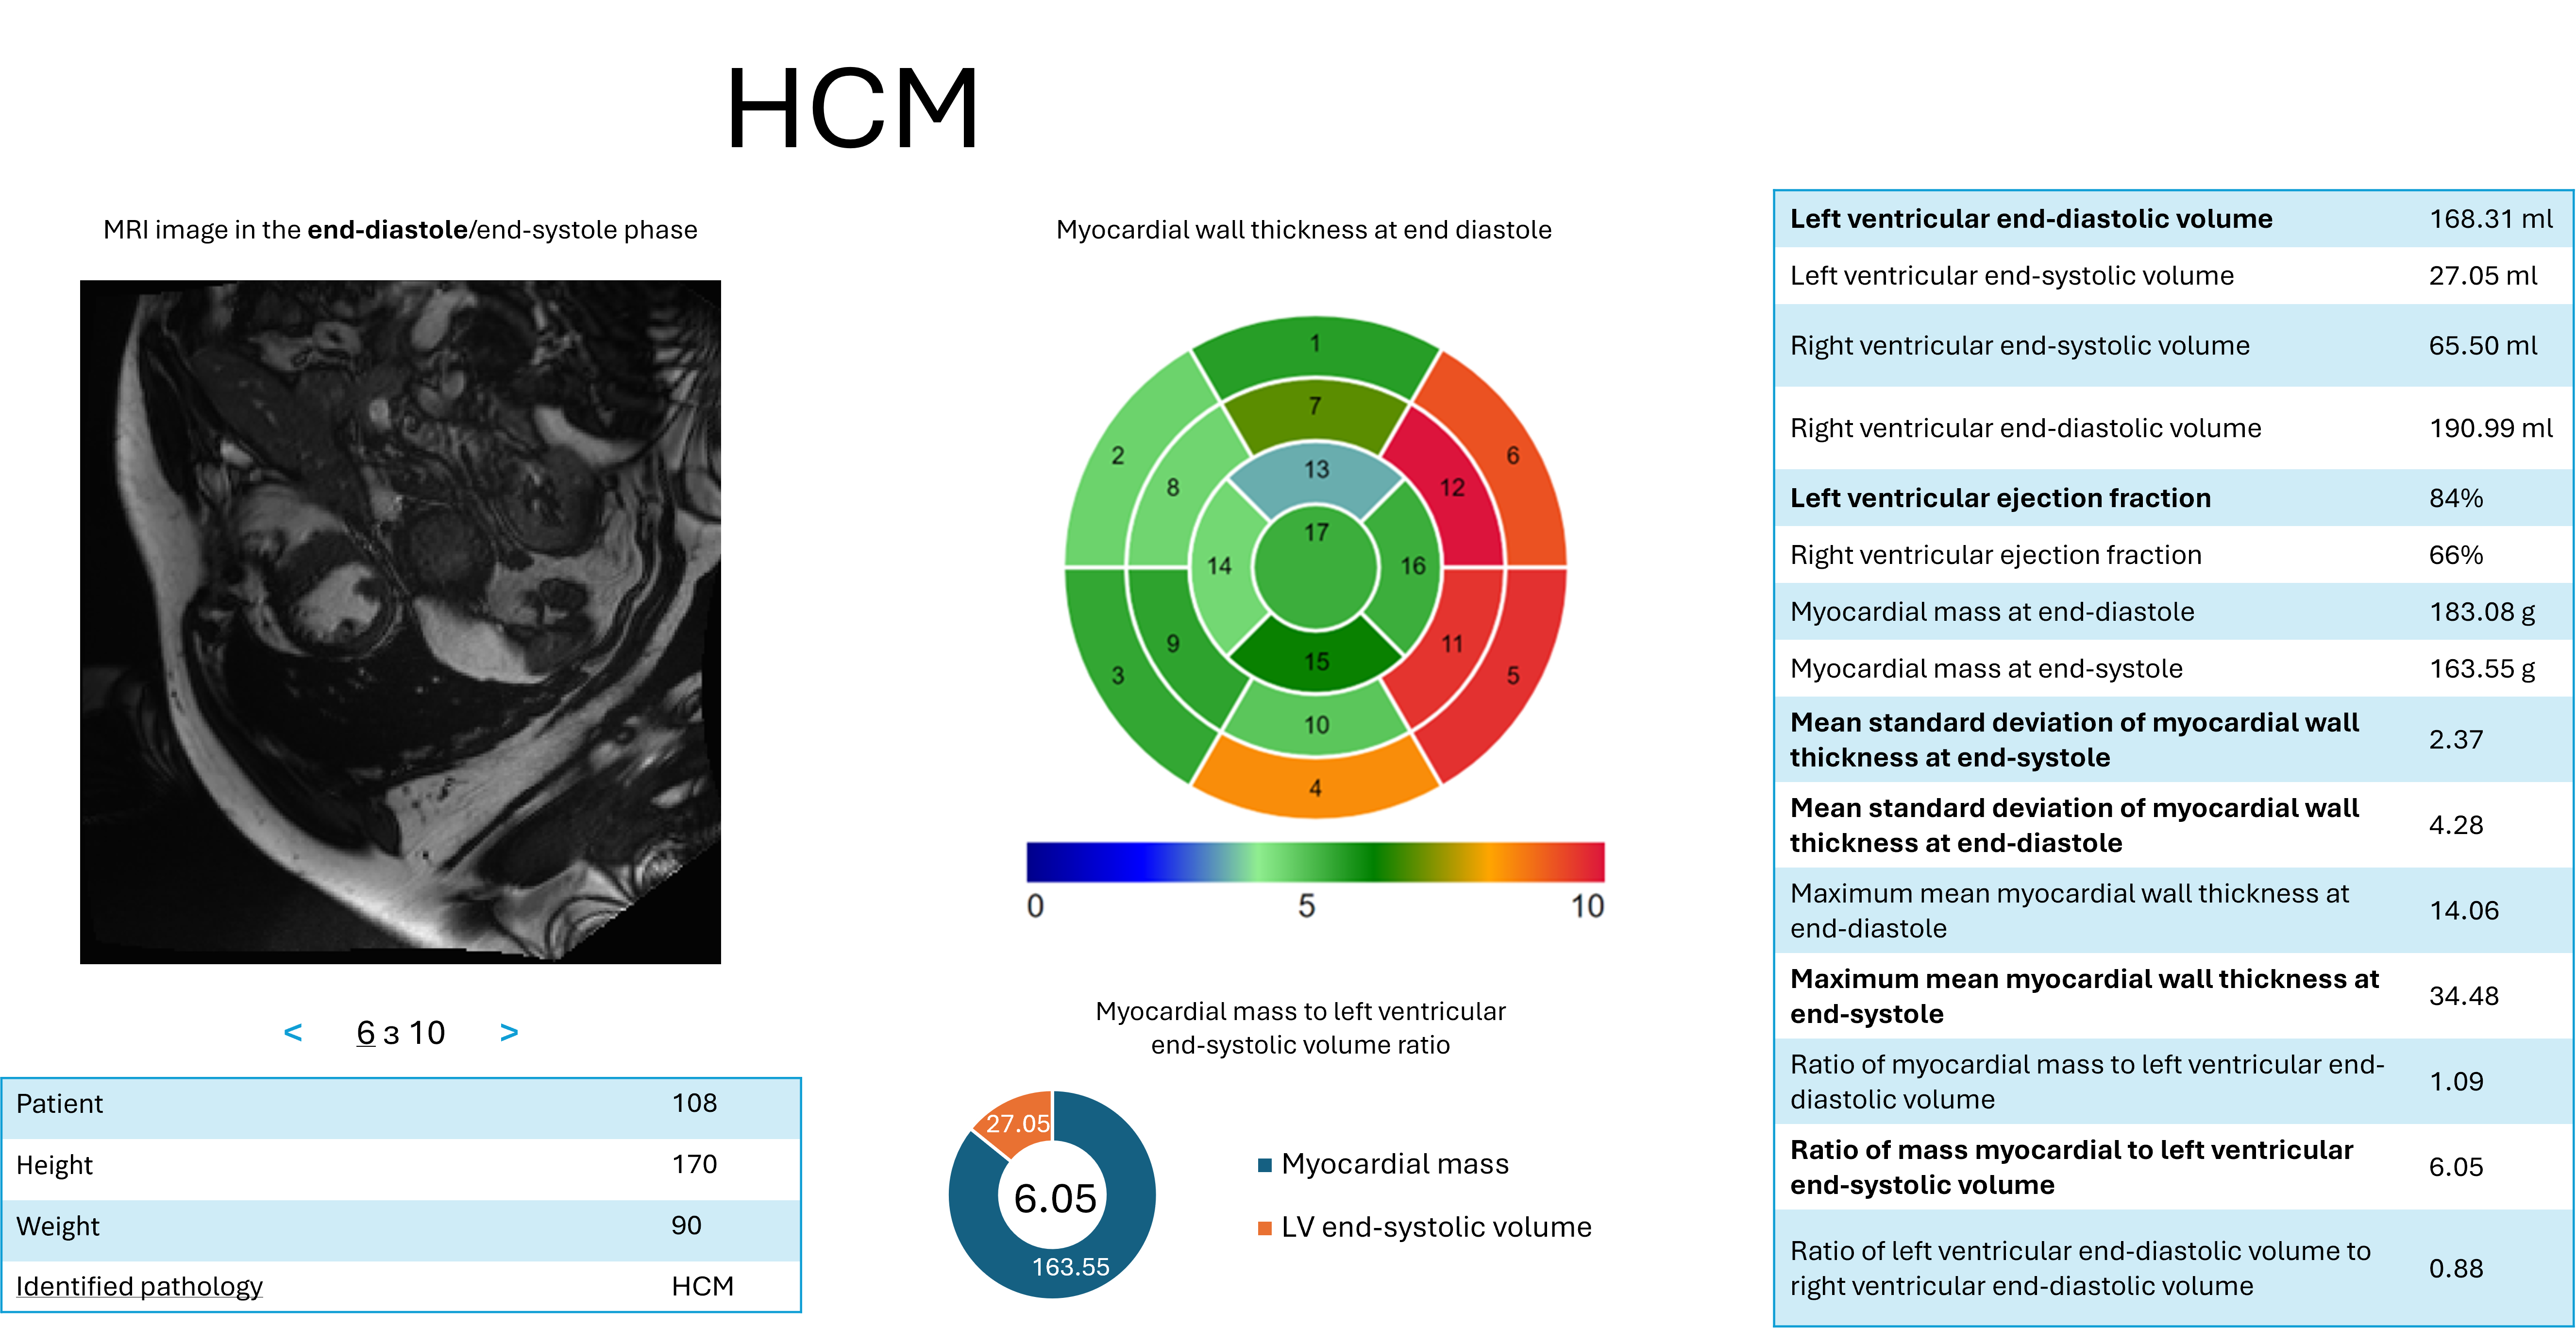
\includegraphics[width=1.0\linewidth]{img/56_fig_s2_HCM.png}
\caption{Visualization of HCM, illustrating thickened myocardial segments and high ejection fraction.}
\label{fig:hcm_visualization}
\end{figure}

\begin{figure}[!htbp]
\centering
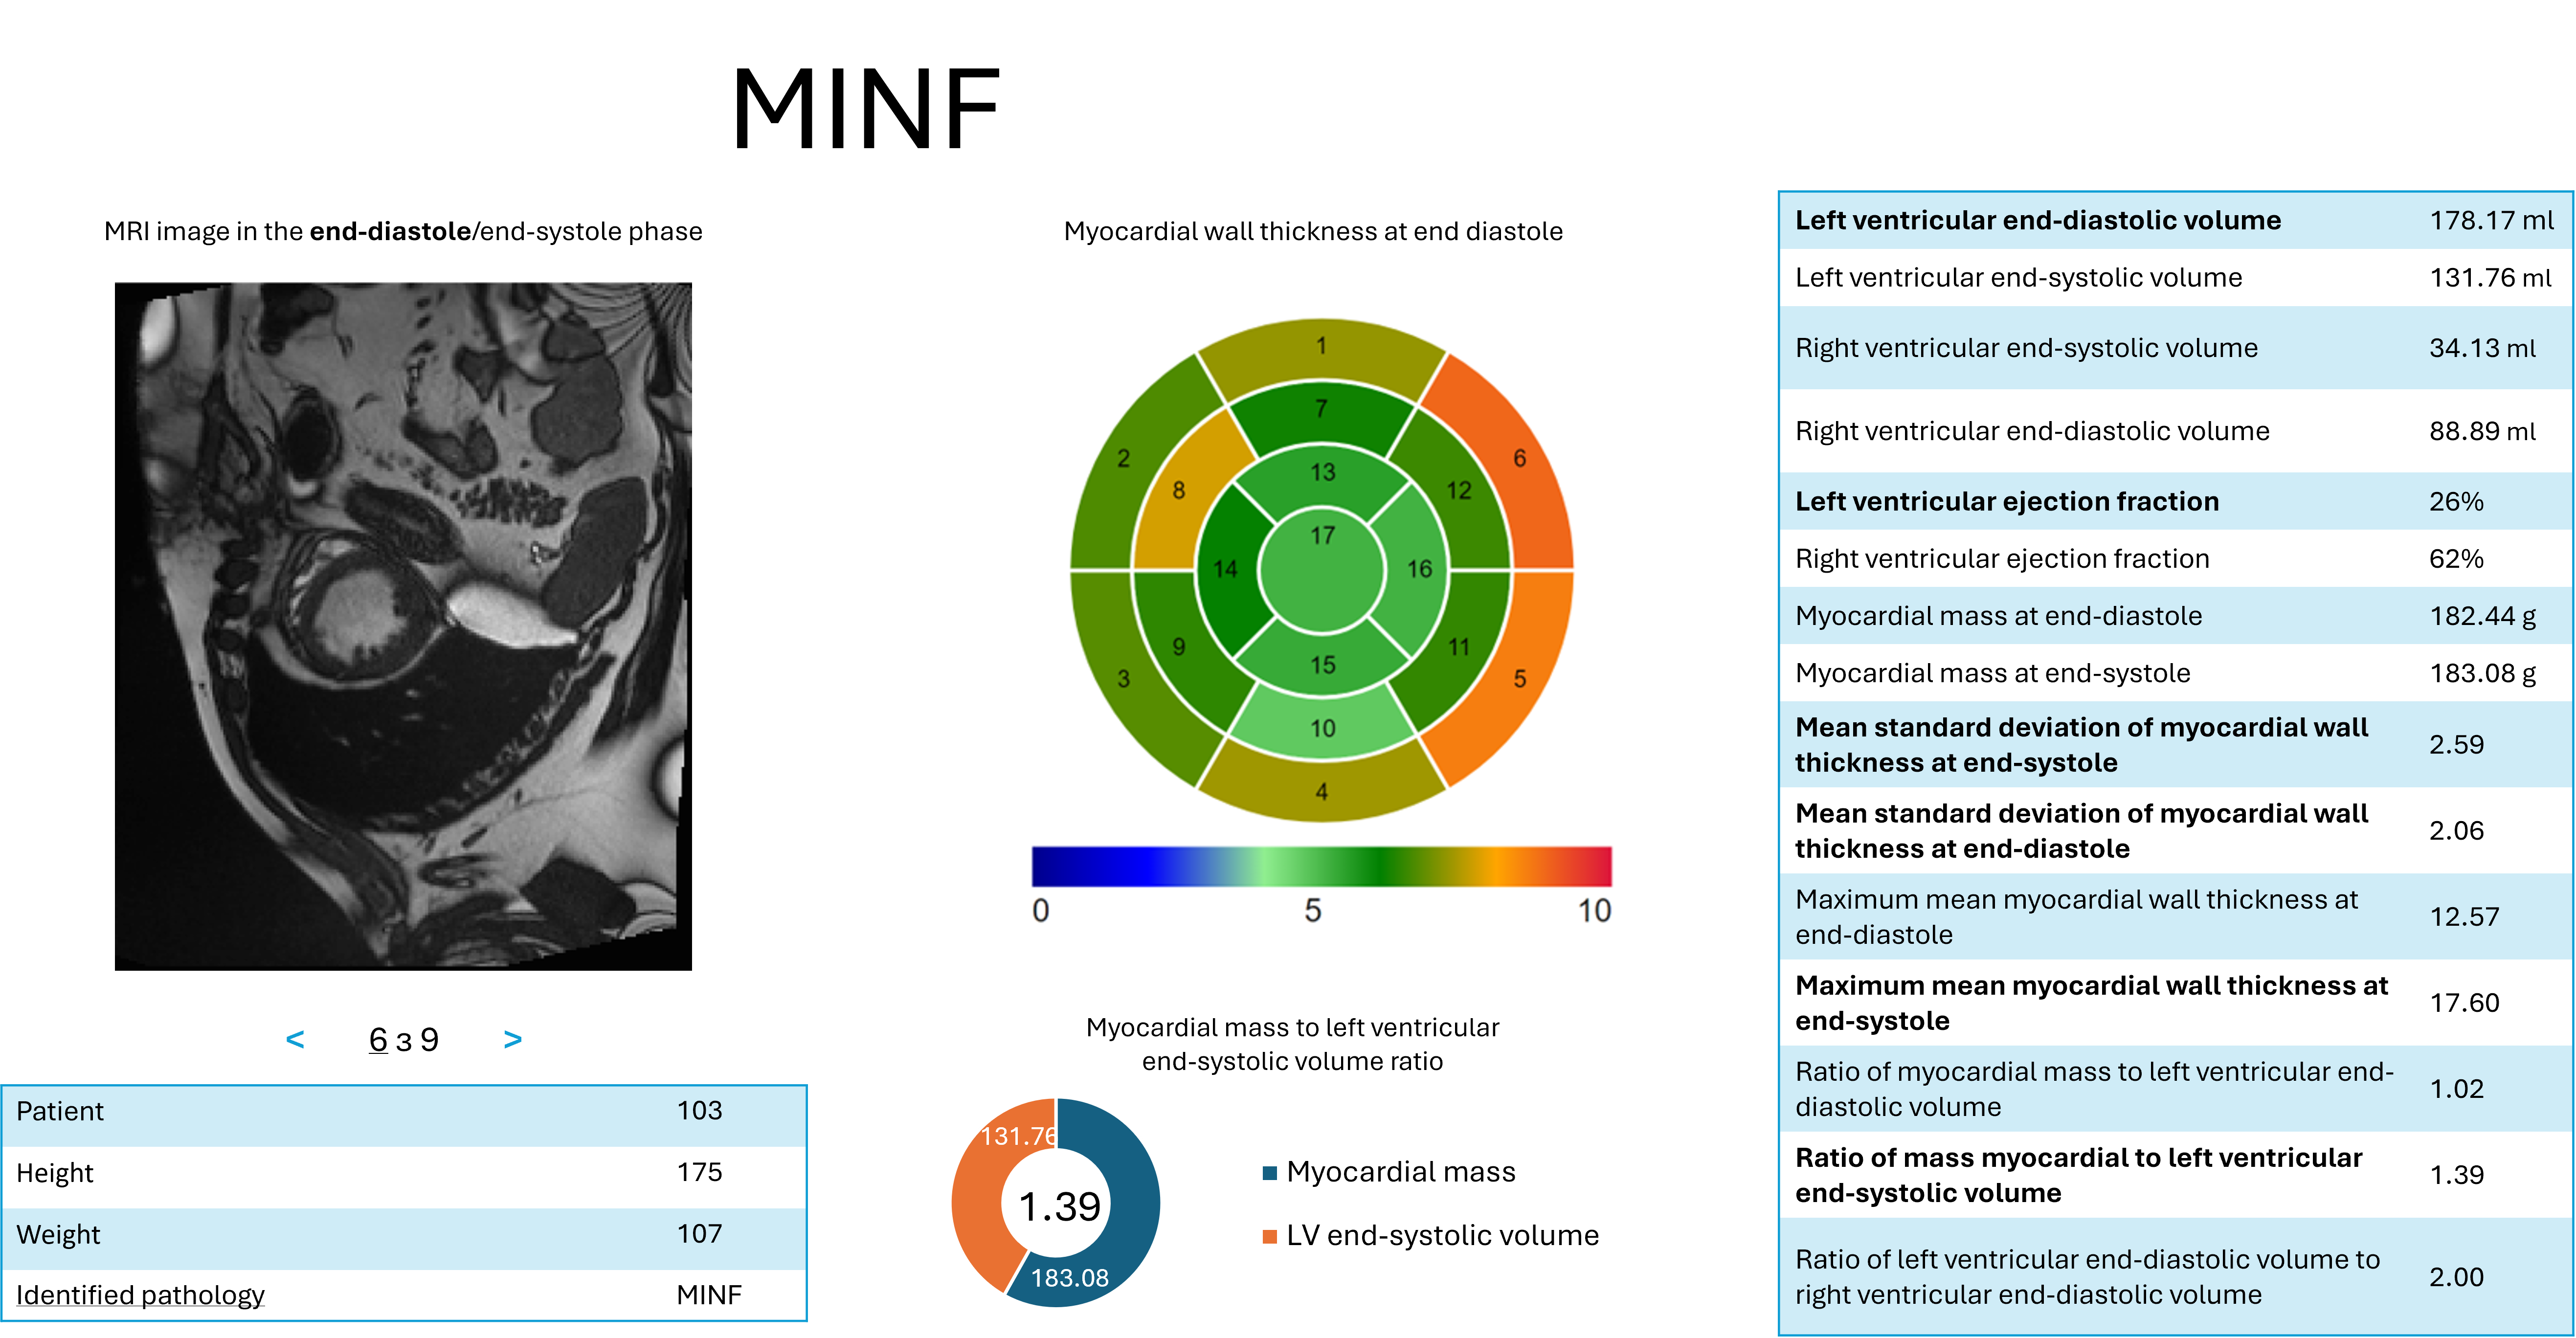
\includegraphics[width=1.0\linewidth]{img/56_fig_s3_MINF.png}
\caption{Visualization of MINF, highlighting reduced ejection fraction and irregular myocardium thickness.}
\label{fig:minf_visualization}
\end{figure}

\begin{figure}[!htbp]
\centering
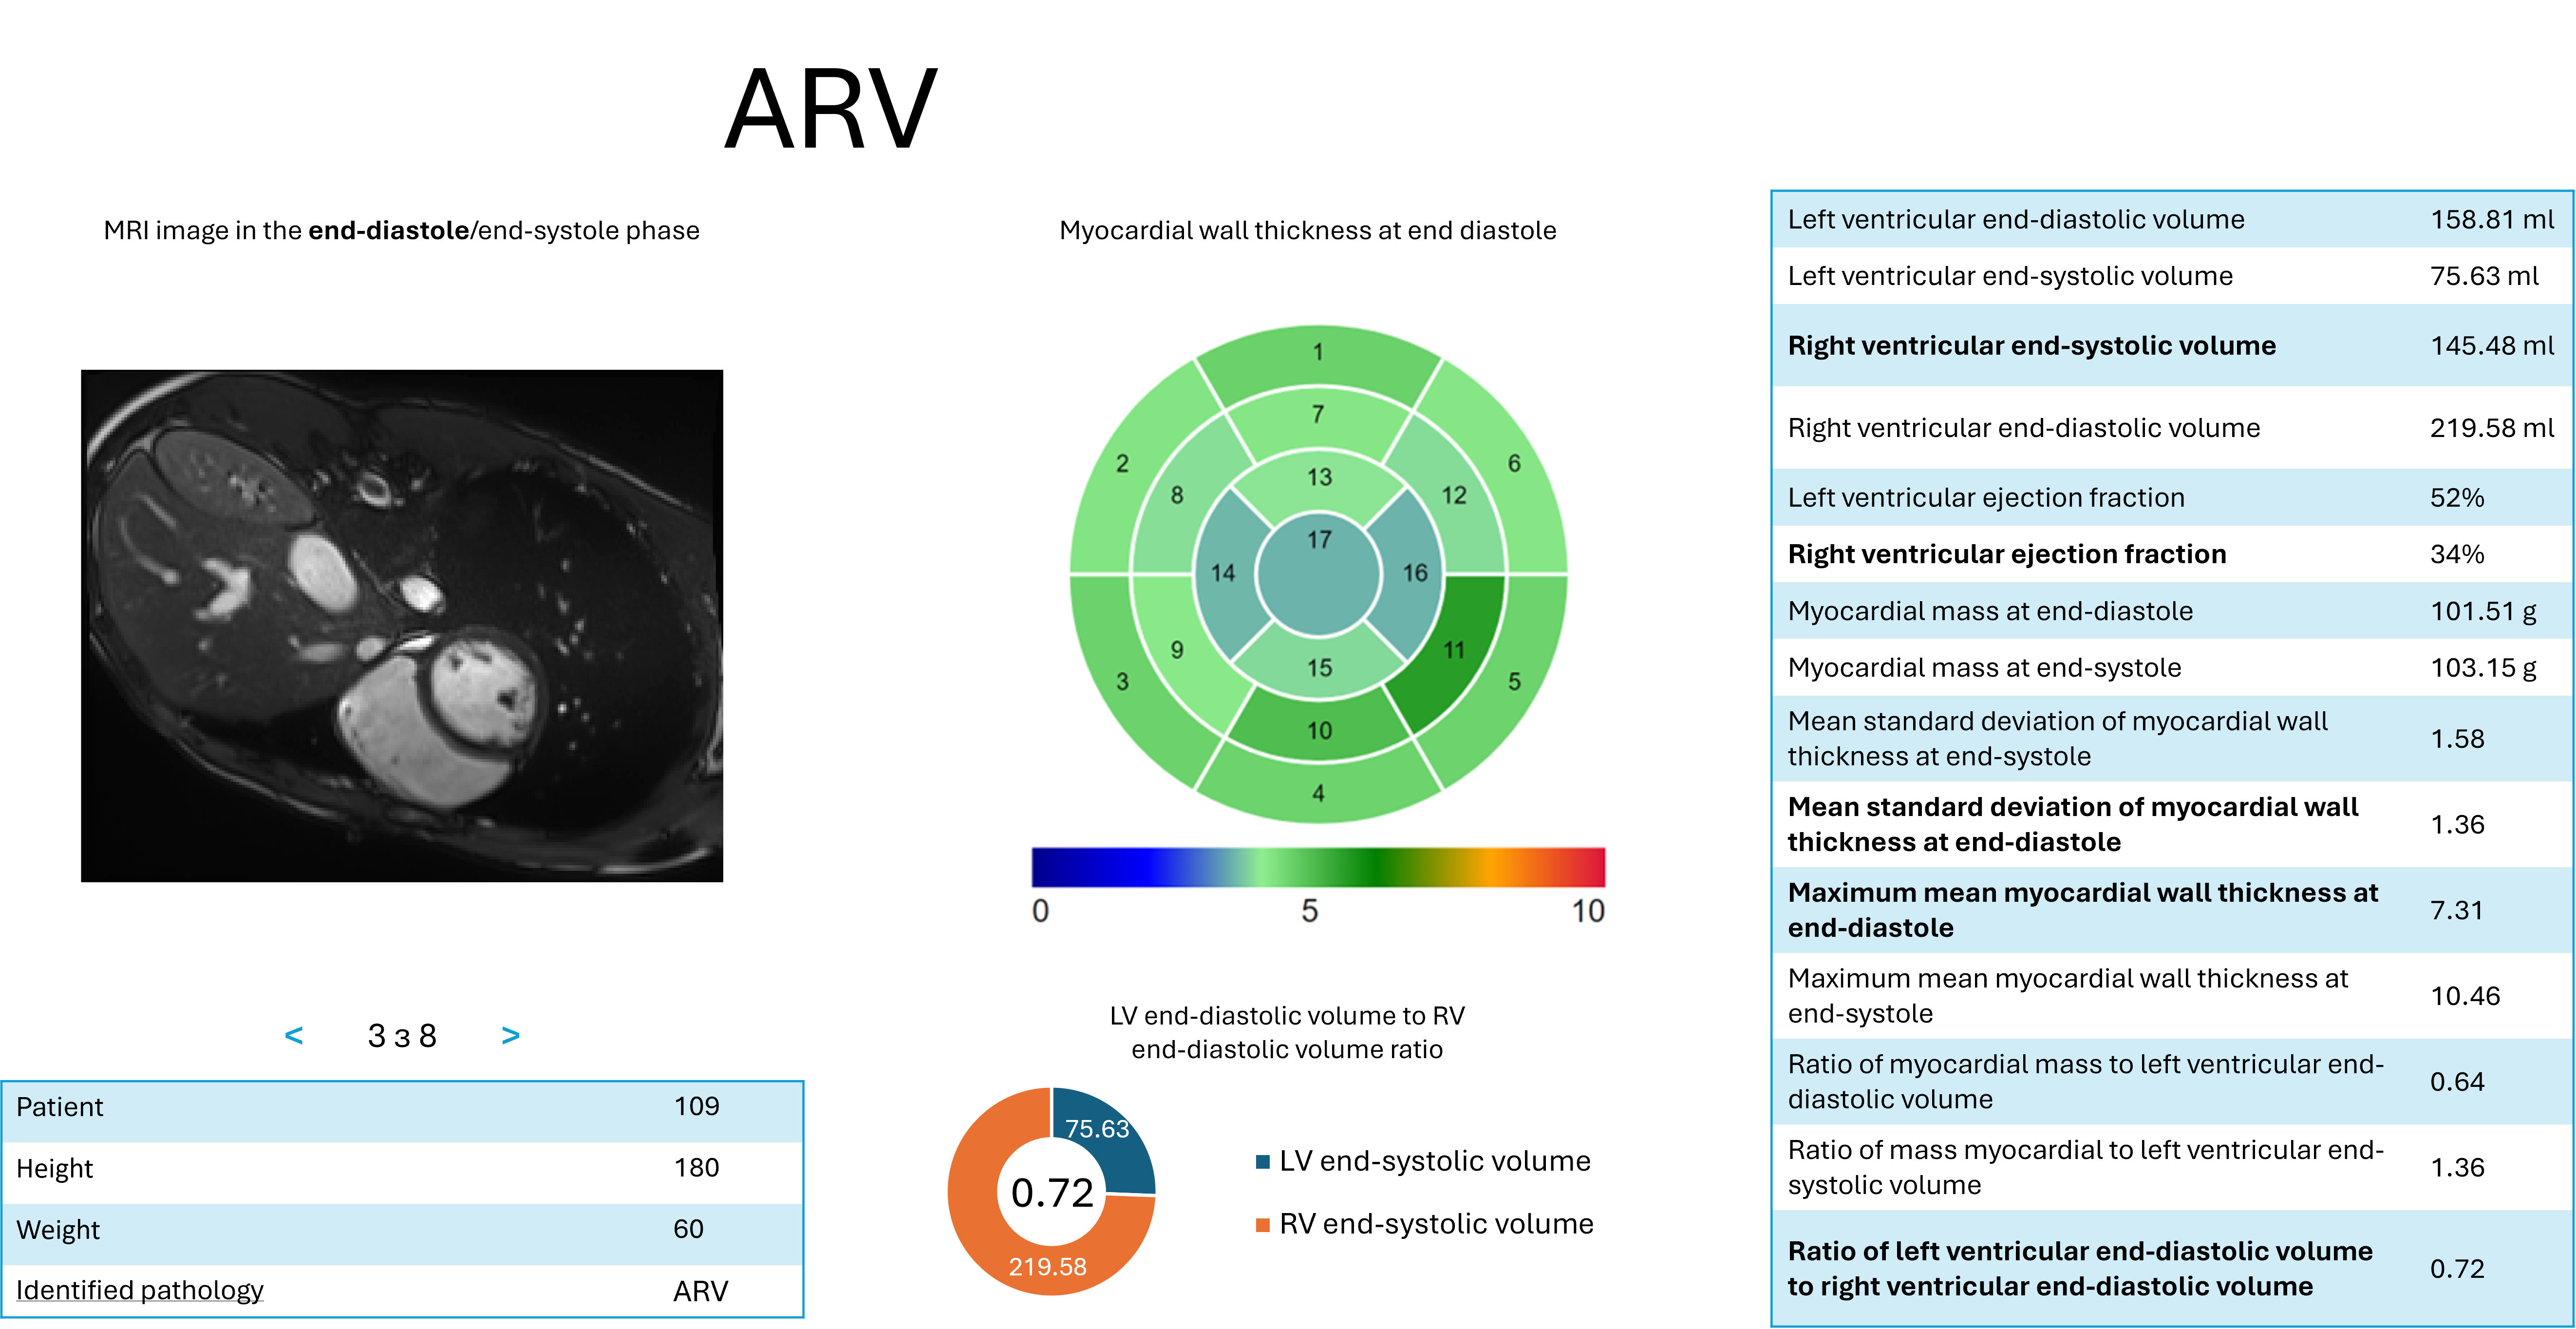
\includegraphics[width=1.0\linewidth]{img/56_fig_s4_ARV.png}
\caption{Visualization of ARV, illustrating enlarged RV and weakened systolic performance.}
\label{fig:arv_visualization}
\end{figure}

\begin{figure}[!htbp]
\centering
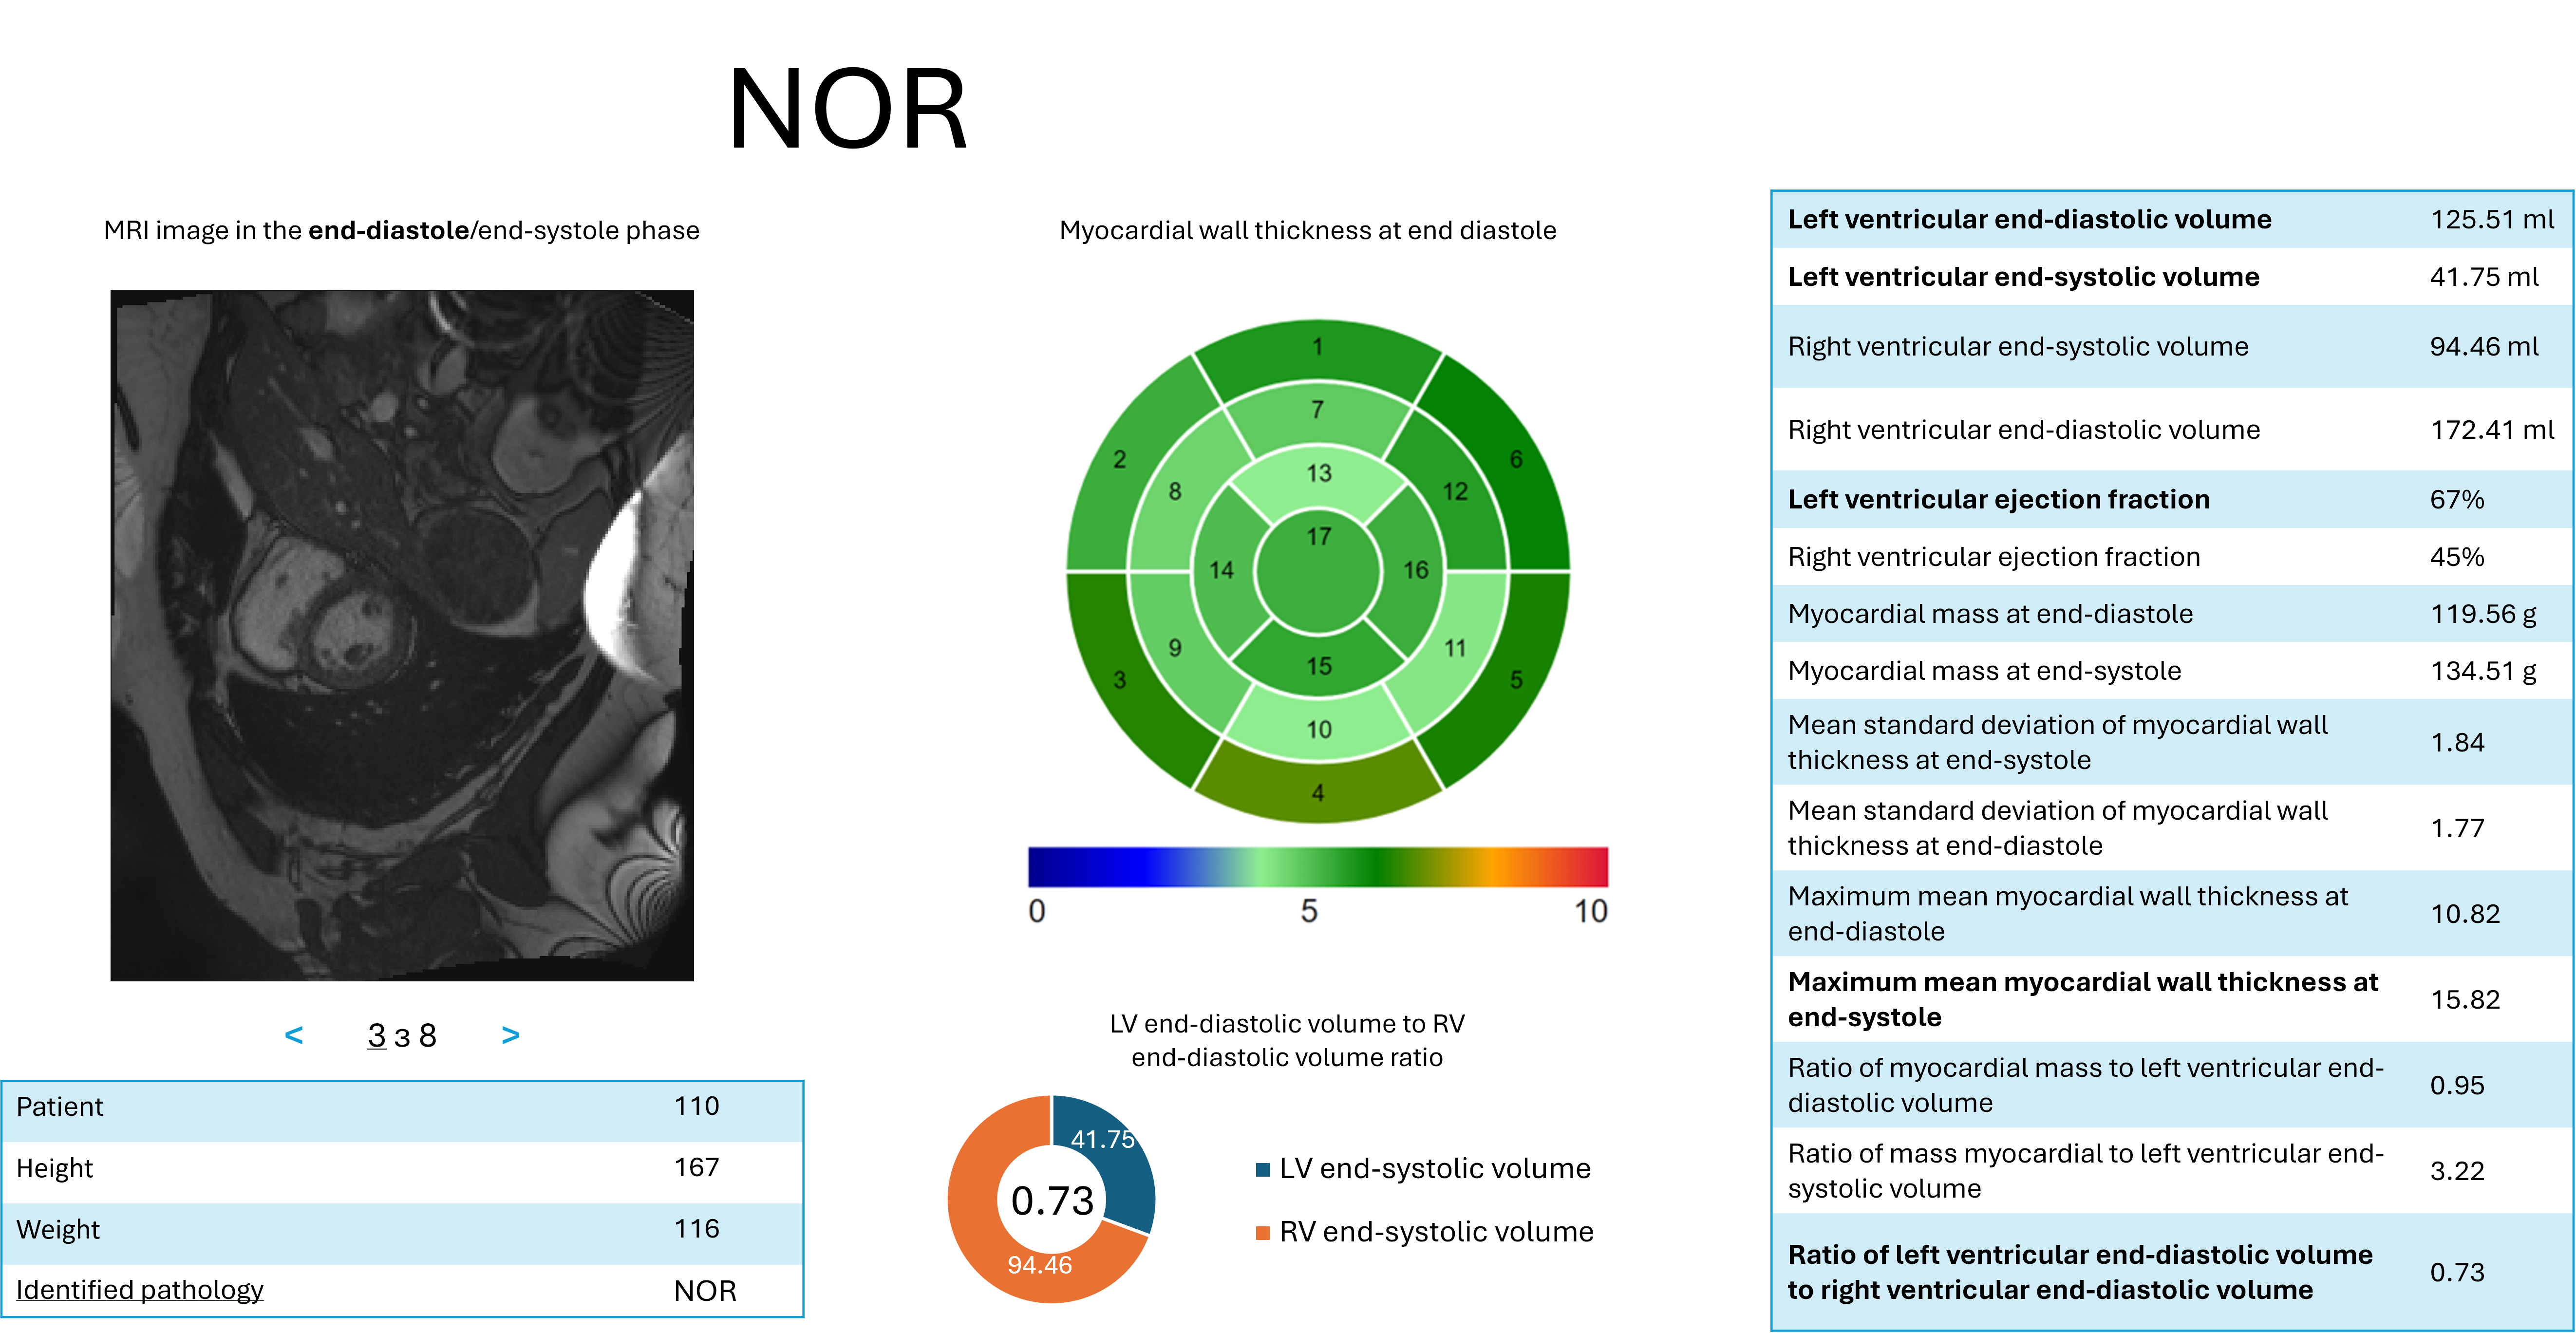
\includegraphics[width=1.0\linewidth]{img/56_fig_s5_NOR.png}
\caption{Visualization of NOR, emphasizing balanced ventricular volumes and normal contractility.}
\label{fig:nor_visualization}
\end{figure}

\Rone{\revtag{1}{5}
\begin{figure}[!htbp]
    \centering
    % In a real submission, a PDF file would be generated and included.
    % \includegraphics[width=\linewidth]{figures/fig_calibration_reliability.pdf} 
    \fbox{\parbox[c][15em][c]{0.9\linewidth}{\centering \huge Placeholder for Reliability Diagrams Figure S6. \\ \large This figure would show four plots, one for each stage of the classification cascade. Each plot would show predicted probability vs. true probability, with bars for each bin, the diagonal line for perfect calibration, and reported ECE/MCE values.}}
    \caption{Calibration of the cascade classifiers. Reliability diagrams for each of the four classification stages show a close alignment between predicted probabilities (x-axis) and the observed fraction of positives (y-axis), indicating that the models are well-calibrated. Shaded bands would show 95\% bootstrap CIs. For Classifier 1, ECE=0.021, MCE=0.045. For Classifier 2, ECE=0.008, MCE=0.015. For Classifier 3, ECE=0.005, MCE=0.011. For Classifier 4, ECE=0.028, MCE=0.052. All values indicate low miscalibration.}
    \label{fig:calibration}
\end{figure}
}


\begin{table}[!htbp]
  \centering
  \caption{\Rtwo{\revtag{2}{2}Dice coefficients by slice position (basal, mid-ventricular, apical) and cardiac phase (ED, ES), evaluated on the ACDC test set. The results show the significant improvement gained by the slice-position-aware refinement module, particularly for the challenging apical and basal slices. Values are mean (95\% CI).}}
  \label{tab:apical_basal_performance}
  \begin{tabular}{lcccccc}
    \toprule
    \multirow{2}{*}{\textbf{Slice Position \& Method}} & \multicolumn{3}{c}{\textbf{ED Dice}} & \multicolumn{3}{c}{\textbf{ES Dice}} \\
    \cmidrule(lr){2-4} \cmidrule(lr){5-7}
    & \textbf{LV} & \textbf{RV} & \textbf{Myo} & \textbf{LV} & \textbf{RV} & \textbf{Myo} \\
    \midrule
    Apical (w/o refinement) & 0.931 & 0.865 & 0.811 & 0.892 & 0.823 & 0.845 \\
    Apical (with refinement) & \textbf{0.958} & \textbf{0.901} & \textbf{0.849} & \textbf{0.925} & \textbf{0.866} & \textbf{0.880} \\
    \midrule
    Mid (w/o refinement) & 0.982 & 0.955 & 0.912 & 0.951 & 0.922 & 0.931 \\
    Mid (with refinement) & \textbf{0.983} & \textbf{0.956} & \textbf{0.915} & \textbf{0.952} & \textbf{0.924} & \textbf{0.933} \\
    \midrule
    Basal (w/o refinement) & 0.945 & 0.889 & 0.833 & 0.908 & 0.850 & 0.871 \\
    Basal (with refinement) & \textbf{0.969} & \textbf{0.920} & \textbf{0.865} & \textbf{0.933} & \textbf{0.881} & \textbf{0.902} \\
    \bottomrule
  \end{tabular}
\end{table}

\section*{Extended Data}
\renewcommand{\thetable}{E\arabic{table}}
\setcounter{table}{0}


\begin{table}[!htbp]
  \caption{\Rtwo{\revtag{2}{3}Diagnostic segmentation performance on the internal ACDC test set versus the external M\&Ms validation set. The model was trained only on ACDC data. Performance drop on M\&Ms reflects the domain shift from different scanner vendors and sites. Classification AUROC on M\&Ms is not applicable (N/A) as the challenge did not provide the same pathology labels. Values are mean (95\% CI).}}
  \label{tab:performance}
  \centering
  \begin{tabular}{lcccc}
    \toprule
    Cohort & LV Dice & RV Dice & MYO Dice & AUROC (cascade) \\
    \midrule
    ACDC (test) & 0.957 (0.95-0.96) & 0.931 (0.92-0.94) & 0.908 (0.90-0.91) & 0.98 (0.97-0.99) \\
    M\&Ms (external) & 0.91 (0.90-0.92) & 0.86 (0.84-0.88) & 0.85 (0.83-0.86) & N/A \\
    \bottomrule
  \end{tabular}
\end{table}


\begin{table}[!htbp]
  \caption{\Rthree{\revtag{3}{7}Papillary-muscle sensitivity analysis at end-diastole (ED). The table shows the impact on calculated Left Ventricular (LV) mass and Ejection Fraction (EF) when papillary muscles are either included within the myocardium or excluded (treated as part of the LV blood pool). Our default policy is exclusion. Values are mean (95\% CI) across the ACDC test set.}}
  \label{tab:papillary_sensitivity}
  \centering
  \begin{tabular}{lcc}
    \toprule
    Setting & LV mass (g) & EF (\%) \\
    \midrule
    Include papillary muscles & 135.2 (131.1-139.3) & 61.5 (59.2-63.8) \\
    Exclude papillary muscles (default) & 124.8 (121.5-128.1) & 62.1 (59.9-64.3) \\
    \bottomrule
  \end{tabular}
\end{table}

\end{document}